\documentclass[11pt]{article}
\usepackage[T1]{fontenc}
\usepackage{lmodern}
\input{glyphtounicode-cmex}
\pdfgentounicode=1
\usepackage[margin=1in]{geometry}
\usepackage{amsmath,amssymb,amsthm,mathtools,mathrsfs}
\usepackage{microtype,xurl}
\usepackage{booktabs,array,longtable,enumitem}
\usepackage[numbers,sort&compress]{natbib}
\usepackage{tikz}
\usetikzlibrary{arrows.meta,positioning,calc,fit}
\usepackage[hypertexnames=false,colorlinks=true,linkcolor=blue!45!black,
  citecolor=blue!45!black,urlcolor=blue!45!black]{hyperref}
\hypersetup{pdftitle={The Mahler Conjecture for General Convex Bodies},
  pdfauthor={OpenAI}}
\newtheorem{theorem}{Theorem}[section]
\newtheorem{lemma}[theorem]{Lemma}
\newtheorem{proposition}[theorem]{Proposition}
\newtheorem{corollary}[theorem]{Corollary}
\theoremstyle{definition}
\newtheorem{definition}[theorem]{Definition}
\theoremstyle{remark}
\newtheorem{remark}[theorem]{Remark}
\newcommand{\E}{\mathbb E}
\newcommand{\R}{\mathbb R}
\newcommand{\N}{\mathbb N}
\newcommand{\ind}{\mathbf 1}
\DeclareMathOperator{\arsinh}{arsinh}
\DeclareMathOperator{\Var}{Var}
\DeclareMathOperator{\Cov}{Cov}
\setlist[enumerate]{itemsep=3pt,topsep=5pt}
\setlist[itemize]{itemsep=3pt,topsep=5pt}
\allowdisplaybreaks[2]
\title{The Mahler Conjecture for General Convex Bodies}
\author{OpenAI}
\date{September 22, 2026}
\begin{document}
\maketitle
\begin{abstract}
We resolve the Mahler conjecture for general convex bodies positively.
For every convex body $K\subset\mathbb R^n$, $n\ge1$, with Santal\'o point
$s(K)$,
$|K|\,|(K-s(K))^\circ|\ge (n+1)^{n+1}/(n!)^2$,
with equality exactly for simplices.

\end{abstract}
\section{Introduction}\label{sec:introduction}

The Mahler conjecture asks which convex bodies have the smallest product
of their volume and the volume of a suitably centered polar body.
We resolve the conjecture positively: simplices are exactly the minimizers
in every positive dimension.

A \emph{convex body} in $\mathbb R^n$ is a compact convex set with nonempty
interior.  We write $|A|$ for the $n$-dimensional Lebesgue volume of a measurable
set $A$, and $\langle\cdot,\cdot\rangle$ for the Euclidean inner product.
For $z\in\operatorname{int}K$, define
\[
 (K-z)^\circ
 =\{y\in\mathbb R^n:\langle y,x-z\rangle\le1\text{ for every }x\in K\}.
\]
The minimum of $|(K-z)^\circ|$ is attained at a unique point
$s(K)\in\operatorname{int}K$, the \emph{Santal\'o point}
(a proof is included in Section~\ref{sec:01-cones}). The volume product is
\[
 P(K)=|K|\,|(K-s(K))^\circ|
     =\inf_{z\in\operatorname{int}K}|K|\,|(K-z)^\circ|.
\]
It is invariant under invertible affine maps.
A simplex is the convex hull of $n+1$ affinely independent points.

\begin{theorem}[General Mahler conjecture]\label{thm:mahler}
For every integer $n\ge1$ and every convex body $K\subset\mathbb R^n$,
\[
                 P(K)\ge\frac{(n+1)^{n+1}}{(n!)^2}.
\]
Equality holds if and only if $K$ is a simplex.
\end{theorem}

Theorem~\ref{thm:mahler} applies without symmetry or boundary regularity assumptions.
It also gives the displayed lower bound for
$|K|\,|(K-z)^\circ|$ at every interior translation point $z$.
The symmetric Mahler conjecture asks for the different, stronger constant
$4^n/n!$ on the restricted class of centrally symmetric bodies; that sharper
statement is separate from Theorem~\ref{thm:mahler} and is proved in the
companion paper \cite[Theorem~1.1]{OpenAISymmetricMahler2026}.

\subsection*{History and context}

The lower-volume-product problem grew out of Mahler's work on polarity
and the geometry of numbers. His polygon paper established the general
planar inequality and its triangle equality case among polygons
\cite{Mahler1938}; his transference paper formulated the
higher-dimensional symmetric problem \cite{Mahler1939}.
Meyer later gave a new proof of the planar general inequality and
completed its equality characterization for arbitrary planar convex
bodies: triangles are exactly the minimizers \cite{Meyer1991}. The affine center used here belongs to the classical
Santal\'o theory \cite{Santalo1949}; we give its elementary existence
and uniqueness argument in Section~\ref{sec:01-cones}.

Several lines of work explain the distinction between an asymptotic lower
bound and the exact simplex constant. The inverse Santal\'o theorem of
Bourgain and Milman gives
$|K|\,|K^\circ|\ge c^n|B_2^n|^2$ for origin-symmetric bodies, where $c>0$ is
absolute and $B_2^n$ is the Euclidean unit ball
\cite{BourgainMilman1987}. Kuperberg obtained explicit lower bounds through
Gauss linking integrals, with separate conclusions in the symmetric and
general settings \cite{Kuperberg2008}. Nazarov developed a complex-analytic
proof using Bergman kernels and H\"ormander estimates
\cite{Nazarov2012}; Mastrantonis and Rubinstein extended that direct
analytical method to nonsymmetric bodies \cite{MastrantonisRubinstein2024}.
These approaches establish exponential-order lower bounds without the
sharp constant asserted in Theorem~\ref{thm:mahler}.

Exact results in substantial special classes also preceded the general
statement. Meyer and Reisner used shadow systems, one-parameter
deformations of convex bodies, to prove the sharp inequality and simplex
equality for polytopes with at most $n+3$ vertices. Their key input is
convexity of the reciprocal polar volume at the Santal\'o point along
such a deformation \cite[Theorems~1 and~10]{MeyerReisner2006}.
Kim and Reisner established strict
local minimality, with a quantitative estimate, at every simplex
\cite[Theorem~1]{KimReisner2011}; this is local information about the
space of convex bodies. In dimension three, Iriyeh and Shibata proved the
symmetric conjecture \cite{IriyehShibata2020}. The 2026 preprint of Chen,
Li, Xi, and Xu proves $P(K)\ge64/9$ for every three-dimensional
convex body, with equality exactly for tetrahedra
\cite{ChenLiXiXu2026}. Their shadow flows constrain the permitted
deformations so that they can treat arbitrary polytopes in dimension
three and then pass to general bodies. In contrast, the argument below
works with projections onto a fixed cone and their Gaussian averages.
Theorem~\ref{thm:mahler} concerns arbitrary convex bodies in all
dimensions, including its global equality classification.

\subsection*{Proof strategy}
The first step is the cone/Laplace correspondence developed by Klartag
\cite[Lemma~2.1 and Corollary~4.1]{Klartag2018}. Choose
$z_0\in\operatorname{int}K$ and put $m=n+1$. Lift the translated body
to the cone
\[
 C=\{(tx,t):t\ge0,\ x\in K-z_0\}\subset\mathbb R^m,
 \qquad D=\{y:\langle y,x\rangle\ge0\text{ for every }x\in C\}.
\]
For $V\in\operatorname{int}D$ and $U\in\operatorname{int}C$, set
$\chi_C(V)=\int_Ce^{-\langle V,x\rangle}\,dx$ and define $\chi_D(U)$
similarly. Section~\ref{sec:01-cones} shows that the desired inequality
follows from $\chi_C(V)\chi_D(U)\ge1$ whenever
$\langle U,V\rangle=m$. We use positive duality and retain the short
calculation to fix the signs and factorials.

The paired maps into $C$ and $D$ arise from Moreau's decomposition
\cite{Moreau1962,Soltan2019}. Let $\Pi_C$ and $\Pi_D$ be Euclidean nearest-point projections, and
write $Z=\Sigma^{1/2}G$, where $G=(G_1,\ldots,G_m)$ is standard Gaussian
and $\Sigma$ is positive definite. For a real layer parameter $z$,
choose a bias $\xi_z$ so that
$X_z=\Pi_C(Z+\xi_z)$ has mean $a(z)U$, where
$a(z)=\mathbb E\max\{g+z,0\}$ for a standard one-dimensional Gaussian $g$.
Its dual partner is $Y_z=\Pi_D(-Z-\xi_z)$.
Section~\ref{sec:02-projections} proves that every such bias exists and
then chooses linear coordinates and the covariance of $Z$
simultaneously. The dependence of the covariance on the projection
field is essential to the later matrix cancellation. Integrating the
projection maps over $z$ gives two injective, smoothed maps into the
cones. Change of variables and Jensen's inequality turn their Jacobians
into a lower bound for the normalized logarithm of the Laplace product
in Section~\ref{sec:03-entropy}. Write this lower bound as
$-\mathcal E$; the remaining task is to prove $\mathcal E\le0$.
Entropy and log-Laplace perturbations also appear in the functional
volume-product work of Fradelizi and Mar\'in Sola
\cite{FradeliziMarinSola2024}; that is a related analytical setting,
not an input theorem for these maps.

The main difficulty is that the derivative matrices $P_z=D\Pi_C(Z+\xi_z)$
need not commute and need not form an increasing family in $z$.
Estimating them independently would discard the information needed for
both the constant and equality. Sections~\ref{sec:04-quadratic}
and~\ref{sec:05-layers} therefore compare the full family to spectral
thresholds of a linear Gaussian matrix $L=\sum_{i=1}^mG_iM_i$, where the
$M_i$ are deterministic symmetric matrices. Classical Hermite expansion
and the Gaussian inverse-generator covariance identity
\cite[Proposition~2.1]{HoudrePrivault2002} separate this
linear part from higher Gaussian degrees. The resulting upper bound
for $\mathcal E$ subtracts a nonnegative layer defect and reduces
all other terms to functions of $L$ and the chosen covariance.

Section~\ref{sec:06-linear-equality} uses the matrix divided-difference
formula to express those functions as averages over pairs of eigenvalues.
A strict scalar inequality on each nontrivial interval absorbs the
remaining errors. Equality then forces the coefficient matrices $M_i$
to commute and the projection derivative to be diagonal in one fixed
basis. The cone splits into one-dimensional half-lines, so its bounded
section is a simplex. The converse is a direct volume computation.

The dimension-independent estimates used in this chain are stated in
Proposition~\ref{prop:scalar-input}. Appendix~\ref{sec:07-scalar} proves
the one-variable and pointwise layer bounds; Appendix~\ref{sec:08-segments}
proves the strict interval inequality. Both include the analytic
interpolation and tail arguments that turn their finite rational
certificates into statements on the whole real line. Numerical sampling
is not used as a substitute for these arguments. Figure~\ref{fig:proof-map}
records the logical dependencies and locates the independent scalar branch.

\begin{figure}[htbp]
\centering
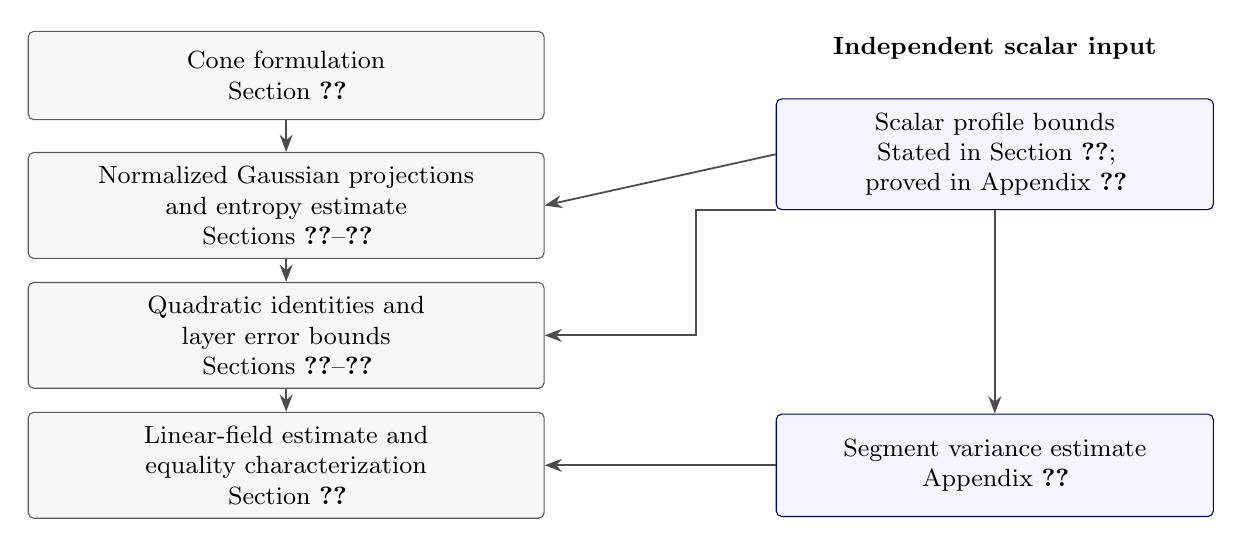
\begin{tikzpicture}[
  font=\small,
  main/.style={draw=black!65,rounded corners=2pt,fill=black!3,
    align=center,text width=6.2cm,minimum height=1.12cm,inner sep=5pt},
  scalar/.style={draw=blue!45!black,rounded corners=2pt,fill=blue!4,
    align=center,text width=5.2cm,minimum height=1.3cm,inner sep=5pt},
  use/.style={-{Stealth[length=2.2mm]},draw=black!70,line width=.65pt}
]
\node[main] (cone) at (0,0)
  {Cone formulation\\Section~\ref{sec:01-cones}};
\node[main] (projection) at (0,-1.65)
  {Normalized Gaussian projections\\and entropy estimate\\
   Sections~\ref{sec:02-projections}--\ref{sec:03-entropy}};
\node[main] (quadratic) at (0,-3.3)
  {Quadratic identities and\\layer error bounds\\
   Sections~\ref{sec:04-quadratic}--\ref{sec:05-layers}};
\node[main] (linear) at (0,-4.95)
  {Linear-field estimate and\\equality characterization\\
   Section~\ref{sec:06-linear-equality}};
\node[align=center,font=\small\bfseries] at (9,.35)
  {Independent scalar input};
\node[scalar] (profiles) at (9,-1)
  {Scalar profile bounds\\
   Stated in Section~\ref{sec:01-cones};\\
   proved in Appendix~\ref{sec:07-scalar}};
\node[scalar] (segments) at (9,-4.95)
  {Segment variance estimate\\Appendix~\ref{sec:08-segments}};
\draw[use] (cone) -- (projection);
\draw[use] (projection) -- (quadratic);
\draw[use] (quadratic) -- (linear);
\draw[use] (profiles) -- (segments);
\draw[use] (profiles.west) -- (projection.east);
\draw[use] (profiles.south west) -| (5.2,-3.3) -- (quadratic.east);
\draw[use] (segments.west) -- (linear.east);
\end{tikzpicture}
\caption{Principal logical dependencies. Arrows indicate where inputs are
used, rather than the order of presentation. The scalar branch is independent
of the cone and dimension; its proofs follow the geometric argument.}
\label{fig:proof-map}
\end{figure}


\subsection*{Functional Mahler inequality}

The functional version replaces a convex body by a log-concave function
and polarity by convex conjugation. For a proper lower-semicontinuous
convex function $\varphi:\R^n\to\R\cup\{+\infty\}$, define its
Fenchel--Legendre transform by
\[
 \varphi^*(y)=\sup_{x\in\R^n}\{\langle x,y\rangle-\varphi(x)\},
 \qquad y\in\R^n.
\]
We use the convention $e^{-\infty}=0$.

\begin{corollary}[Functional Mahler inequality]\label{cor:functional-mahler}
For every integer $n\ge1$ and every proper lower-semicontinuous convex
function $\varphi:\R^n\to\R\cup\{+\infty\}$ such that
$0<\int_{\R^n}e^{-\varphi(x)}\,dx<\infty$,
\[
 \left(\int_{\R^n}e^{-\varphi(x)}\,dx\right)
 \left(\int_{\R^n}e^{-\varphi^*(y)}\,dy\right)\ge e^n.
\]
The second integral is allowed to be infinite, in which case the
inequality is immediate.
\end{corollary}

This sharp lower bound applies to general log-concave functions through
their convex potentials; no centering or normalization of $\varphi$ is
required. Its derivation uses Theorem~\ref{thm:mahler} in all dimensions,
not only in dimension $n$, through the implication of Fradelizi and
Meyer \cite[Proposition~2(a)]{FradeliziMeyer2008}.
Section~\ref{sec:consequences} gives the proof, an extremizing example,
and the distinction between geometric and functional equality cases.

The same functional bound has an entropy--transport consequence: for
full-dimensional log-concave probability measures whose densities vanish
at $\mathcal H^{n-1}$-almost every boundary point of their supports
(the essential-continuity condition), it bounds their summed entropies relative to
Lebesgue measure by a transport cost between the distributions of their
potential gradients, with additive constant $-3n$. The precise
definitions and statement appear in Corollary~\ref{cor:entropy-transport}.
This consequence uses the functional equivalence of Gozlan, as stated
in \cite[Theorem~1.3]{FradeliziGozlanZugmeyer2021}; essential continuity
is an additional hypothesis, not a requirement on the convex bodies in
Theorem~\ref{thm:mahler}.

\tableofcontents
\section{Polarity, cone reduction, and the scalar input}\label{sec:01-cones}

We first express the volume product as a product of Laplace integrals on
dual cones. This relation is the one used by Klartag
\cite[Lemma~2.1 and Corollary~4.1]{Klartag2018}, with positive duality and
a normalization adapted to the Gaussian argument. We include the
calculation to fix the signs and factorials. The rest of the proof
estimates the integrals after a suitable linear change of coordinates.

\subsection{The center of polarity}
For completeness we establish the minimizing-center convention used in
Theorem~\ref{thm:mahler}. The support function of a convex body $K$ is
$h_K(u)=\sup_{x\in K}\langle u,x\rangle$. Polar coordinates give, for
$z\in\operatorname{int}K$ and $n\ge2$,
\[
 |(K-z)^\circ|=\frac1n\int_{S^{n-1}}
      (h_K(u)-\langle z,u\rangle)^{-n}\,d\sigma(u),
\]
where $\sigma$ is surface measure on the unit sphere.
This is strictly convex as a function of $z$: the function $t\mapsto t^{-n}$
is strictly convex for $t>0$, and for any two distinct centers their
inner products differ on a set of positive surface measure.
It also tends to infinity as $z$ approaches the boundary of $K$.
Indeed, at a limiting boundary point choose a unit supporting normal $u_0$.
Then $\varepsilon=h_K(u_0)-\langle z,u_0\rangle\to0$.
The support functions $h_K(u)-\langle z,u\rangle$ have a common Lipschitz
constant for $z\in K$. On a spherical cap of radius $\varepsilon$ about
$u_0$, their values are at most a constant times $\varepsilon$.
The cap has measure at least a constant times $\varepsilon^{n-1}$,
so its contribution to the integral is at least a constant times
$\varepsilon^{-1}$. Existence and uniqueness of an interior minimizer
follow. In dimension one the same conclusion follows directly from
$(z-a)^{-1}+(b-z)^{-1}$ for $K=[a,b]$.

For an invertible affine map $x\mapsto Bx+a$,
\[
 (BK+a-(Bz+a))^\circ=B^{-\mathsf T}(K-z)^\circ.
\]
The two volume factors change by reciprocal determinants. This proves
affine invariance of the volume product and the equivariance
$s(BK+a)=Bs(K)+a$.

\subsection{The cone formulation}
Put \(m=n+1\). For \(z_0\in\operatorname{int}K\), define
\[
C=\{(y,t):t\ge0,\ y\in t(K-z_0)\},\qquad
D=C^*=\{w:\langle w,x\rangle\ge0\text{ for all }x\in C\}.
\]
For cones, the star denotes this \emph{positive} duality. Both cones are closed, convex, solid, and pointed: solid means having nonempty interior, and pointed means containing no line. For interior vectors \(V\in D\) and \(U\in C\), write
\[
 \chi_C(V)=\int_C e^{-\langle V,x\rangle}\,dx,\qquad
 \chi_D(U)=\int_D e^{-\langle U,x\rangle}\,dx
\]
using \(m\)-dimensional Lebesgue measure.

\begin{lemma}[Cone reduction]\label{lem:cone-reduction}
For \(U=(0,m)\) and \(V=(0,1)\),
\[
\chi_C(V)\chi_D(U)=\frac{(n!)^2}{m^m}|K|\,|(K-z_0)^\circ|.
\]
For any closed convex solid pointed cone and any interior pair \(U\in C\), \(V\in C^*\), the two Laplace integrals are finite. Their product and the inner product \(\langle U,V\rangle\) are preserved by
\[
(C,D,U,V)\longmapsto(BC,B^{-\mathsf T}D,BU,B^{-\mathsf T}V)
\]
for every invertible linear map \(B\).
\end{lemma}
\begin{proof}
A point \((w,t)\) lies in \(D\) exactly when
\(t\ge\sup_{x\in K-z_0}\langle-w,x\rangle\). Since zero is interior to \(K-z_0\), this forces \(t\ge0\), and the slice at height \(t\) is \(-t(K-z_0)^\circ\). Integrating the slices gives
\[
\chi_C((0,1))=n!|K|,\qquad
\chi_D((0,m))=n!m^{-m}|(K-z_0)^\circ|.
\]
For general cone data, interiority of \(V\) gives \(\langle V,x\rangle\ge c|x|\) on \(C\), and interiority of \(U\) gives the analogous estimate on \(D\). These inequalities prove finiteness. Under the displayed transformation, the two change-of-variables factors are \(|\det B|\) and \(|\det B|^{-1}\), and the inner products in the exponential factors are unchanged.
\end{proof}

It therefore suffices to prove
\[
             \chi_C(V)\chi_D(U)\ \ge\ 1,                            \tag{1}\label{eq:1}
\]
whenever \(C\subset\mathbb R^m\) is closed, convex, solid, and pointed, \(D=C^*\), \(U\in\operatorname{int}C\), \(V\in\operatorname{int}D\), and \(\langle U,V\rangle=m\). These will be the standing cone assumptions. We will also show that equality implies that \(C\) is a linear image of an orthant; Section~\ref{sec:06-linear-equality} completes the equality argument for the original body.

The proof constructs two maps from Gaussians using projections on the cones. To control their Jacobians we compare the whole field of projection derivatives to matrix thresholds, with a linear Gaussian matrix as threshold variable. A small feedback in the Gaussian covariance will be used to handle functions of that linear matrix. In the cone argument \(C,D\) refer to cones, while \(\mathsf K,\mathsf C\) below are scalar profiles and \(\mathbf K,\mathbf C\) will be expectations of their symmetric-matrix evaluations. Real layer indices such as \(z\) in the projection field are separate from the Gaussian vector input.

\subsection{Scalar profiles and their identities}
The estimates will use fixed scalar functions, independent of the cone and its dimension. Write \(\phi(x)=(2\pi)^{-1/2}e^{-x^2/2}\), \(p(x)=\int_{-\infty}^x\phi(y)\,dy\), and \(\gamma f=\int f(x)\phi(x)\,dx\). Put \(\mathcal N=x\partial_x-\partial_x^2\). To define three profiles, temporarily write \(X=p/\phi\), \(Y=(1-p)/\phi\), \(f=-(1-p)-\log p\), and \(j=-p-\log(1-p)\). Set
\[
 d=(1+xX)^2 f+(1-xY)^2 j,\qquad
 g=\tfrac12(1-X^2 f-Y^2 j),\qquad v=\log(XY).
\]
\begin{lemma}[Profile identities]\label{lem:profile-identities}
The functions just defined satisfy
\[
 (\mathcal N+2)g=d,\qquad d'=2xd-v'-2g',\qquad
 \mathcal N d-v''=-(\mathcal N+2)(d+g'').                          \tag{2}\label{eq:2}
\]
\end{lemma}
\begin{proof}
We have \(X'=1+xX\), \(Y'=xY-1\), \(f'=-\phi(1-p)/p\), and \(j'=\phi p/(1-p)\). Direct substitution gives
\[
X^2f'+Y^2j'=0,\qquad XX'f'+YY'j'=-1,\qquad
(X')^2f'+(Y')^2j'=-v'.
\]
Also \(X''=xX'+X\) and \(Y''=xY'+Y\). Thus
\(g'=-(XX'f+YY'j)\), and differentiating once more proves \((\mathcal N+2)g=d\). Differentiating \(d=(X')^2f+(Y')^2j\) proves its stated first-order identity. Finally, differentiating the first identity twice gives \(d''=(\mathcal N+4)g''\); combining this with the derivative of the second identity proves the third.
\end{proof}

\subsection{The quantitative scalar inequalities}

The parameters used are (finite decimals throughout denote exact numbers)
\[
\begin{gathered}
 b=.602,\quad c=.365,\quad k=\sqrt{b-c},\quad r=.22,\quad w=4.6,\quad s=3.6,\\
 \eta=.022,\quad \kappa=1.16,\quad \lambda=.65,\quad a_R=7.5,\\
 t_-=-.022,\quad t_+=.064,\quad t_c=.021,\quad t_r=.043,\quad m_*=.352.
\end{gathered}
\]
Define
\[
\begin{aligned}
 \mathsf K&=d-2g,\qquad \mathsf C=-d+(a_R-1)g'',\\
 \pi(x)&=r(\cos(w\operatorname{arsinh}(x/s)),\sin(w\operatorname{arsinh}(x/s))),\\
 q(x)&=k-\sqrt{b-r^2-d(x)},\qquad u=(\pi,q),\qquad S_u=(2+\mathcal N)u=(S_\pi,S_q),\\
 F&=d+|u|^2=c+2kq.
\end{aligned}
\]
The key algebraic choice is that $d+|u|^2$ is affine in $q$.
It will allow a quadratic profile correction to be estimated through one
component. The circular part of $u$ supplies variation on every
nontrivial segment; Appendix~\ref{sec:08-segments} quantifies that fact.
The parameters are fixed independently of the body and dimension.
The first group of inequalities below permits the covariance choice,
the second controls errors from the projection layers, and the third
controls the spectral interval averages of the linear Gaussian field.
Their constants are not asserted to be optimal. The argument uses
precisely the following inequalities, which we collect as one input. Their proofs appear in Appendices~\ref{sec:07-scalar} and~\ref{sec:08-segments}. A bar over a function with specified endpoints denotes its uniform average on that segment, or its value when the endpoints coincide.

\begin{proposition}[Scalar inequalities]\label{prop:scalar-input}
The profiles and exact parameters above have the following properties.

\noindent\textbullet\quad \(b-r^2-d>0,\ |v'-x|\le .319,\ \mathsf C\le-.341,\ S_q>0\), and
\[
 \lambda t_-^2+t_-\mathsf C+\mathsf K>0,\qquad
 \lambda t_+^2+t_+\mathsf C+\mathsf K<0,\qquad
 2(-.37)\mathsf C-(.37)^2-4\lambda\mathsf K>m_*^2 .
\]
\noindent\textbullet\quad Write
\[
 \begin{aligned}
 b_m&=\frac{(1+t_+)(b-3\eta)}{3(3(b+\eta)-4c)},\qquad
 e_0=.256,\qquad \alpha=2.26,\qquad h_s=.5,\\
 H(z,x)&=4c+4kq(x)+2(k-q(x))S_q(z)-2S_\pi(z)\cdot\pi(x),\qquad
 H_0(z,x)=H(z,x)+v''(x)-2\kappa .
 \end{aligned}
\]
Pointwise,
\[
\begin{aligned}
 H+t_c H_0-\tfrac12t_r(h_s+H_0^2/h_s) >
  2(b+\eta+(b+\eta-\kappa)t_-)+2 b_m S_q(z)S_q(x)+2e_0(2t_r)^2+H_0^2/\alpha,\\
 4c+2k(S_q(z)+S_q(x))-S_q(z)S_q(x)-S_\pi(z)\cdot S_\pi(x) >0 .
\end{aligned}                                                       \tag{3}\label{eq:3}
\]
\noindent\textbullet\quad For endpoints \(x_-<x_+\), use subscripts \(\sigma\in\{-,+\}\) for evaluations, with \(-\sigma\) the opposite endpoint. Then
\[
\begin{aligned}
 e_K+\Gamma&+
 \frac{1}{8\lambda}\sum_\sigma
 (\overline{\mathsf C}-\mathsf C_{-\sigma}-\overline{|u-u_\sigma|^2})^2
 +\frac{t_+}{2}\sum_\sigma|\bar u-u_\sigma|^2
 <\overline{|u|^2}-|\bar u|^2,\\
 e_K&=\overline{\mathsf K}-(\mathsf K_++\mathsf K_-)/2,\\
 \Gamma&=\frac{.80}{m_*^2}
 \big[1.25(\mathsf K_+-\mathsf K_-+t_c(\mathsf C_+-\mathsf C_-))^2+
           5 t_r^2(\mathsf C_+-\mathsf C_-)^2\big].
\end{aligned}                                                       \tag{4}\label{eq:4}
\]
For coincident endpoints the two sides in the inequality are equal.
\end{proposition}

The first set of inequalities permits the covariance choice in Section~\ref{sec:02-projections}. The function \(v\) enters the entropy estimate, where Equation~\eqref{eq:2} expresses its contribution through \(d\) and \(g\). The identity \(d+|u|^2=F\) and the two-variable and segment inequalities are used in the later quadratic and spectral estimates. In particular \(d,g,v,q\) are even, as follows from their definitions.

We will also use that these profiles are smooth and that their derivatives
have at most polynomial growth. The exponentially large factor \(X\) does
not make the profiles grow exponentially: its occurrences can be rewritten
in terms of the Gaussian tail ratio \(Y\). On \(x\ge0\),
\(Y=\int_0^\infty e^{-xy-y^2/2}dy\) is comparable to \((1+x)^{-1}\),
and \(1-xY=O((1+x)^{-2})\). Set
\(h_0(y)=(-\log(1-y)-y)/y^2\), with its smooth value at zero.
At \(y=1-p\), the relevant formulas are
\[
 (1+xX)^2f=(1-p(1-xY))^2h_0(y),\qquad
 X^2f=Y^2p^2h_0(y),\qquad j=-p-\log(Y\phi).
\]
Differentiating the Laplace integral for \(Y\) gives bounds for its
derivatives; these formulas then give polynomial derivative bounds for
\(d,g,v,\mathsf K,\mathsf C\). Reflection supplies the negative half-line.
Moreover, \(d\to1/2\) at both ends. The radicand in \(q\) therefore
tends to \(b-r^2-1/2=.0536>0\). Its positivity in
Proposition~\ref{prop:scalar-input}, together with continuity on compact
intervals, gives a uniform positive lower bound. Differentiation of the
square root is thus legitimate globally and gives the same growth property
for \(q\). The bounds for \(\pi\) follow directly from its explicit
formula, and those for \(F\) follow from \(F=d+|u|^2\).
Appendix~\ref{sec:07-scalar}
provides the quantitative bounds used here. No such growth claim is made
for the temporary factors \(X,Y\) separately.

In the cone argument below, a smooth scalar test always means that the
test and all its derivatives have at most polynomial growth. We use
natural logarithms. Matrix inequalities for symmetric matrices are in
quadratic form order.

\section{Biased projections and simultaneous normalization}\label{sec:02-projections}

We now construct a family of projections whose means follow a prescribed curve in the cone. Its derivative field will provide both the Jacobians in the entropy argument and the matrix fields in the quadratic estimates. The final step of this section chooses coordinates and a Gaussian covariance simultaneously.

\subsection{The biased projection field}
For now fix the cone data satisfying the standing assumptions of Section~\ref{sec:01-cones}, and a symmetric matrix \(T\) with \(t_-I\le T\le t_+I\). Set
\[
\Sigma=I+T,\qquad Z=\Sigma^{1/2}G,
\]
where \(G\) is standard Gaussian in \(\mathbb R^m\). Thus every eigenvalue of \(\Sigma\) lies in \([.978,1.064]\). Expectations refer to \(G\), unless another variable is specified. For matrix fields use
\[
\tau B=\frac1m\mathbb E\operatorname{tr}B,\qquad
\tau_\Lambda B=\tau(\Lambda B),\qquad
\langle B,E\rangle_\Lambda=\tau_\Lambda(B\circ E),\qquad
B\circ E=\tfrac12(BE+EB).
\]
Here \(B,E\) are symmetric and \(\Lambda\) is a deterministic symmetric weight; the same notation applies to deterministic matrices. Transposition and cyclicity give \(\operatorname{tr}(\Lambda BE)=\operatorname{tr}(\Lambda EB)\). We suppress the subscript \(I\). For arbitrary square matrix fields write \(\|B\|_2^2=\tau(B^{\mathsf T}B)\), and put \([B,E]=BE-EB\).

Let \(\Pi_C\) denote Euclidean nearest-point projection onto \(C\), and put \(a(z)=\phi(z)+zp(z)\), so that \(a>0\) and \(a'=p\).

\begin{lemma}[Biased projections]\label{lem:biased-projections}
For every \(z\in\mathbb R\) there is a unique vector \(\xi_z\) such that
\[
X_z=\Pi_C(Z+\xi_z),\qquad Y_z=\Pi_D(-Z-\xi_z),\qquad
\mathbb EX_z=a(z)U.\tag{5}\label{eq:5}
\]
The map \(z\mapsto\xi_z\) is smooth. The a.e. derivative
\(P_z=D\Pi_C(Z+\xi_z)\) is a symmetric positive contraction, and
\[
X_z-Y_z=Z+\xi_z,\qquad X_z\cdot Y_z=0,\qquad
(\mathbb EP_z)\xi_z'=p(z)U.
\]
Define
\[
B(z)=\frac1m U\cdot\mathbb EY_z,\quad r_1(z)=-B'(z),\quad
h(z)=\tau_\Sigma P_z,\quad s_0=\tau\Sigma.
\]
Then
\[
\begin{gathered}
h(z)=\frac1m\mathbb E(X_z\cdot Z)
=\frac1m\mathbb E|X_z-\mathbb EX_z|^2+a(z)B(z),\\
h'=pB+ar_1,\qquad r_1>0.
\end{gathered}\tag{6}\label{eq:6}
\]
\end{lemma}
\begin{proof}
Moreau's cone decomposition, with the positive-dual convention, gives
\(\Pi_C(w)-\Pi_D(-w)=w\) and orthogonality of the two terms
\cite{Moreau1962,Soltan2019}. Here is the sign convention directly.
Writing $x=\Pi_C(w)$, the projection variational inequality is
$\langle w-x,c-x\rangle\le0$ for $c\in C$. Taking $c=0,2x$ gives
$\langle w-x,x\rangle=0$; the same inequality then gives $y=x-w\in D$.
For $d\in D$, $\langle-w-y,d-y\rangle=-\langle x,d\rangle\le0$,
so $y=\Pi_D(-w)$. Applying the projection inequality to two inputs
also gives
$|\Pi_C(w)-\Pi_C(w')|^2\le\langle\Pi_C(w)-\Pi_C(w'),w-w'\rangle$,
hence the projection is one-Lipschitz. It is the gradient of the convex function
\[
\Phi(w)=\tfrac12|\Pi_C(w)|^2
=\sup_{x\in C}\bigl(\langle w,x\rangle-\tfrac12|x|^2\bigr).
\]
Rademacher's theorem gives its a.e. differentiability
\cite{Rademacher1919,NekvindaZajicek1988}. A Lipschitz function is
absolutely continuous on coordinate lines; one-dimensional integration
by parts and Fubini's theorem identify these derivatives with the weak
derivatives. The convex-gradient representation therefore makes the
a.e. derivative symmetric and positive semidefinite, and the Lipschitz
bound makes it at most \(I\). Symmetry can equivalently be seen from commutation of weak mixed derivatives.

For fixed \(a>0\), minimize
\(\Psi_a(\xi)=\mathbb E\Phi(Z+\xi)-aU\cdot\xi\).
Write the orthogonal cone decomposition of \(\xi\) as \(\xi=x-y\). Since \(U\) is interior to \(C\), there is \(c>0\) with \(U\cdot y\ge c|y|\) for \(y\in D\). Jensen's inequality gives
\[
\Psi_a(\xi)\ge\tfrac12|x|^2-a|U||x|+ac|y|.
\]
This lower bound is coercive. Gaussian convolution makes \(\Psi_a\) smooth, with Hessian \(\mathbb E D\Pi_C(Z+\xi)\). This Hessian is strictly between \(0\) and \(I\): the nondegenerate Gaussian assigns positive probability to open subsets of \(\operatorname{int}C\), where the derivative is \(I\), and of \(-\operatorname{int}D\), where it is zero. Thus the minimizer is unique, and its stationarity condition is \(\mathbb EX=aU\). The implicit function theorem proves smooth dependence on \(z\) and the displayed formula for \(\xi_z'\).

Choose a measurable bounded symmetric-contraction representative for the derivative where it is undefined. For each layer these exceptional inputs are Gaussian-null; Fubini's theorem makes the choice immaterial to all layer integrals. Such a representative can be chosen jointly measurably by using difference quotients for the projection.

Gaussian integration by parts gives \(\mathbb E(X_z\cdot Z)=\mathbb E\operatorname{tr}(\Sigma P_z)\). Since \(\mathbb EY_z=aU-\xi_z\), orthogonality gives
\[
\mathbb E(X_z\cdot Z)=\mathbb E|X_z|^2-aU\cdot\xi_z.
\]
Subtracting \(|\mathbb EX_z|^2\) proves the variance expression in Equation~\eqref{eq:6}. Moreover, \(\nabla|\Pi_C|^2=2\Pi_C\), so
\[
\frac d{dz}\mathbb E|X_z|^2=2aU\cdot\xi_z',\qquad
h'=\frac1m(aU\cdot\xi_z'-pU\cdot\xi_z)=pB+ar_1.
\]
Finally,
\[
r_1=\frac p m U\cdot\bigl((\mathbb EP_z)^{-1}-I\bigr)U>0.
\]
No commutation of \(\Sigma\) with \(\mathbb EP_z\) is used.
\end{proof}

\subsection{Tails and layer integrals}
We need estimates that allow integration over all layers, despite possible nonsmoothness of the cone boundary. In Lemma~\ref{lem:projection-tails}, constants are locally uniform over invertible linear transformations of the fixed cone data, and uniform over the spectral box for \(T\). They may depend on the dimension.

\begin{lemma}[Gaussian layer tails]\label{lem:projection-tails}
For every finite \(r\ge1\), there are \(c_r,C_r>0\) such that
\[
\begin{aligned}
\|P_z\|_{L^r}+\|X_z\|_{L^r}&\le C_re^{-c_rz^2}&& (z\le0),\\
\|I-P_z\|_{L^r}+\|Y_z\|_{L^r}&\le C_re^{-c_rz^2}&& (z\ge0).
\end{aligned}
\]
Here any fixed finite-dimensional matrix norm can be used. Also \(B(z)\le C(1+|z|)\) for \(z\le0\). The positive measure \(\mu=h'(z)\,dz\) has total mass \(s_0\) and all polynomial moments. The measures with densities \(ar_1\) and \(pr_1\) have all polynomial moments as well.
\end{lemma}
\begin{proof}
Interiority and Equation~\eqref{eq:5} give
\[
\mathbb E|X_z|\le Ca(z),\qquad \mathbb E|Y_z|\le CB(z).
\]
For any one-Lipschitz vector function \(F\),
\(|F(Z)|\le\mathbb E|F(Z)|+\mathbb E|Z|+|Z|\); apply this to both projections. For \(s\ge0\),
\[
a(-s)=\phi(s)\int_0^\infty t e^{-st-t^2/2}\,dt
\asymp\frac{\phi(s)}{(1+s)^2},\qquad
p(-s)\le C\frac{\phi(s)}{1+s}.
\]
The lower bound follows by restricting the integral to \([0,(1+s)^{-1}]\); for the upper bound omit one or the other exponential factor. On \([0,\infty)\), \(a(z)\asymp1+z\).

For negative \(z\), split \(\mathbb E(X_z\cdot Z)\) at \(|Z|=C_0(1+|z|)\). The first part is bounded by \(C(1+|z|)a(z)\). In the second part the pointwise Lipschitz bound and Gaussian tails give the same bound when \(C_0\) is sufficiently large. Hence
\[
0\le h(z)\le C(1+|z|)a(z),\qquad B(z)\le h(z)/a(z)\le C(1+|z|).
\]
Since \(0\le P_z\le I\) and \(\Sigma\ge.978I\), this gives Gaussian decay of every finite moment of \(P_z\). The first moment of \(X_z\) is Gaussian-small, while the Lipschitz bound gives bounded moments of arbitrarily high order on the negative half-line. Interpolation gives the asserted decay of its \(L^r\) norms.

For positive \(z\), Equation~\eqref{eq:6} gives \(aB\le h\le s_0\), and thus
\[
|\mathbb EY_z|\le Cs_0/a(z),\qquad \xi_z=a(z)U-\mathbb EY_z.
\]
A fixed interior ball about \(U\) shows that \(\xi_z\) is a distance at least \(cz\) from the complement of \(C\) for all sufficiently large \(z\). On \(|Z|<cz\) the projection is the identity, so \(Y_z=0\) and \(P_z=I\) almost surely. Gaussian tails and the pointwise Lipschitz bound prove the remaining estimates.

The monotone function \(h\) tends to \(0\) and \(s_0\) at the two ends, with Gaussian tails. Integrating these tail functions proves the mass and moment assertions for \(\mu\). Finally \(ar_1\le h'\), and \(p/a\) has polynomial growth, proving the corresponding assertions for the other two densities.
\end{proof}

For a smooth scalar test \(f\) as in Section~\ref{sec:01-cones}, define
\[
\begin{gathered}
H_f=\int_{\mathbb R}(p(z)I-P_z)f'(z)\,dz,\qquad \iota(z)=z,\\
A=H_\iota,\qquad M_i=\mathbb E G_iA,\qquad
L=\sum_{i=1}^mG_iM_i,\qquad R=A-L.
\end{gathered}\tag{7}\label{eq:7}
\]
Lemma~\ref{lem:projection-tails} makes these layer integrals convergent in every finite \(L^r\), and all the displayed matrix fields have all finite moments.

\begin{lemma}[The Gaussian Sobolev interface]\label{lem:projection-sobolev}
For every smooth \(f\) with polynomially bounded derivatives, the centered vector field
\[
W_f=\int_{\mathbb R}(p(z)Z-X_z+\mathbb EX_z)f'(z)\,dz
\]
converges in Gaussian \(W^{1,2}\), and its weak Jacobian in \(G\) is
\(D_GW_f=H_f\Sigma^{1/2}\).
\end{lemma}
\begin{proof}
At negative layers the integrand tends to zero in \(L^2\) at a Gaussian rate. At positive layers use
\[
X_z-\mathbb EX_z=Z+Y_z-\mathbb EY_z
\]
to write it as \((p(z)-1)Z-Y_z+\mathbb EY_z\), with the same decay. The weak Jacobian of the integrand is \((p(z)I-P_z)\Sigma^{1/2}\), whose \(L^2\) norm has integrable Gaussian tails as well. Thus the truncated integrals and their weak derivatives are Cauchy in \(L^2\); closedness of the weak derivative gives the claim. Each integrand is centered. This argument differentiates the Lipschitz projections, not their derivative fields \(P_z\).
\end{proof}

For comparison, when \(C\) is the nonnegative orthant, \(U\) is the all-ones vector, and \(T=0\), one has \(\xi_z=zU\) and
\[
P_z=\operatorname{diag}(1_{\{-G_i\le z\}}),\qquad
A=L=\operatorname{diag}(-G_i).
\]
Indeed \(\int_{\mathbb R}(p(z)-1_{\{v_0\le z\}})\,dz=v_0\). In the general case the family \(P_z\) is neither assumed nested nor assumed to consist of projections. The field \(L\) is its deterministic-coefficient, degree-one Gaussian comparison.

\subsection{Choosing coordinates and covariance}
The remaining task is to arrange both a mean balance for \(A\) and a matrix equation for \(T\).

\begin{proposition}[Simultaneous normalization]\label{prop:normalization}
A linear transformation of the cone data and a symmetric \(T\) in the prescribed spectral box can be chosen so that
\[
\begin{gathered}
\mathbb EA=0,\qquad \lambda T^2+\mathbf C\circ T+\mathbf K=0,\qquad
\mathbf H:=-\mathbf C-2\lambda T\ge m_*I,\\
\mathbf C=\mathbb E\mathsf C(L),\qquad \mathbf K=\mathbb E\mathsf K(L).
\end{gathered}\tag{8}\label{eq:8}
\]
Matrix functions here and below use spectral calculus for symmetric matrices.
\end{proposition}
\begin{proof}
We use the scalar bounds in Proposition~\ref{prop:scalar-input}. For a
symmetric matrix \(Q\), transform the original data by
\[
 C_Q=e^QC_{\rm in},\qquad D_Q=e^{-Q}D_{\rm in},\qquad
 U_Q=e^QU_{\rm in},\qquad V_Q=e^{-Q}V_{\rm in}.
\]
Lemma~\ref{lem:cone-reduction} preserves the Laplace product and
\(U_Q\cdot V_Q=m\). Let \(T\) vary over its spectral box. For each
pair \((Q,T)\), construct the biases and fields as above; we suppress
their dependence on \(Q,T\) in the notation. We first establish
continuity, then construct a continuous self-map and exclude its fixed
points on a sufficiently large \(Q\)-sphere.

\paragraph{Continuity.}
Under convergent invertible transformations the cone projections converge uniformly on compact sets. To see this, projected points are bounded by the norm of the input; subsequential limits belong to the limiting cone and minimize the limiting distance, so uniqueness identifies the limit. Equicontinuity upgrades the conclusion to compact-uniform convergence. The coercive lower bound in Lemma~\ref{lem:biased-projections} is locally uniform, so the biases also converge at every fixed layer.

There is no need to assert pointwise convergence of the derivatives of these projections. Gaussian integration by parts instead gives
\[
\begin{aligned}
(\mathbb EP_z)\Sigma^{1/2}&=\mathbb E X_zG^{\mathsf T},\\
(\mathbb E G_iP_z)\Sigma^{1/2}
&=\mathbb E X_z(G_iG^{\mathsf T}-e_i^{\mathsf T}),
\end{aligned}
\]
where \(e_i\) is the \(i\)-th coordinate vector. The pointwise Lipschitz bounds dominate these expectations locally in the parameters. Lemma~\ref{lem:projection-tails}, also with a Gaussian factor \(G_i\) by H\"older's inequality, permits integration over layers. Hence \(\mathbb EA\) and all \(M_i\) are continuous. Their local boundedness and the polynomial growth of the profiles then give continuity of \(\mathbf C,\mathbf K\).

\paragraph{The covariance update.}
Put \(\Delta=\mathbf C^2-4\lambda\mathbf K\), and set
\[
T_{\rm new}=\frac{-\mathbf C-\sqrt\Delta}{2\lambda}.
\]
The scalar inequalities, spectral calculus, and expectation imply
\[
\begin{gathered}
\Delta\ge m_*^2I,\\
(\mathbf C+2\lambda t_+I)^2\le\Delta
\le(\mathbf C+2\lambda t_-I)^2.
\end{gathered}
\]
For the first inequality use \((\mathbf C+.37I)^2\ge0\). For the other two, expand the squares and use the corresponding endpoint inequalities in Proposition~\ref{prop:scalar-input}. Moreover \(\mathbf C+2\lambda t_\pm I<0\), since \(\mathbf C\le-.341I\) and \(2\lambda t_+=.0832\).

The L\"owner--Heinz inequality states that positive square root is order
preserving, including for noncommuting matrices
\cite[Theorem~2.3]{Chansangiam2013}. Indeed its integral representation uses the order-preserving matrices \(B(B+tI)^{-1}\). Taking square roots in the preceding sandwich therefore gives
\[
-\mathbf C-2\lambda t_+I\le\sqrt\Delta
\le-\mathbf C-2\lambda t_-I,
\]
so \(t_-I\le T_{\rm new}\le t_+I\). The positive discriminant gap also gives continuity of this update.

\paragraph{A uniform inward estimate.}
We claim that
\(\operatorname{tr}(Q\mathbb EA)<0\) whenever \(\sigma=\|Q\|_{\rm Frob}\) is sufficiently large, uniformly over its eigenbasis and over \(T\) in the box. All constants in this paragraph depend only on the original cone data and the fixed dimension, not on \(Q,T\).

Diagonalize \(Q\), write its eigenvalues as \(d_j\), and put \(h_j(z)=\mathbb E(P_z)_{jj}\). Applying the original interior-vector bounds to \(e^{-Q}X_z\) and \(e^QY_z\) gives
\[
\mathbb E|(X_z)_j|\le Ca(z)e^{d_j},\qquad
\mathbb E|(Y_z)_j|\le CB(z)e^{-d_j}.
\]
Gaussian integration by parts in this basis gives
\(h_j=\mathbb E[(X_z)_j(\Sigma^{-1}Z)_j]\), and the analogous identity for \(1-h_j\) uses \(-Y_z\). The covariance bounds and the one-Lipschitz coordinate bounds imply, for every cutoff \(J\ge1\),
\[
\begin{aligned}
h_j&\le CJ\mathbb E|(X_z)_j|+Ce^{-cJ^2},\\
1-h_j&\le CJ\mathbb E|(Y_z)_j|+Ce^{-cJ^2}.
\end{aligned}
\]
For example, bound \(|(X_z)_j|\) by its absolute mean plus \(\mathbb E|Z|+|Z|\), and split the Gaussian integral at \(|Z|=J\). A tail term containing the absolute mean is absorbed by the first term. These bounds require no commutation of \(Q\) and \(\Sigma\).

Set \(A_j=\int_{\mathbb R}(p-h_j)\,dz\) and
\(\varepsilon=1/\sqrt m\). The quantity to be made negative is
\(\operatorname{tr}(Q\mathbb EA)=\sum_jd_jA_j\).
Thus a negative eigenvalue requires a lower bound on \(A_j\), whereas
a positive eigenvalue requires an upper bound. We obtain a uniform bound
for each sign and then improve it when \(|d_j|\ge\varepsilon\sigma\).

If \(d_j\le0\), use \(J=1+|z|\) on the negative half-line in the
estimate for \(h_j\). The bound
\(\mathbb E|(X_z)_j|\le Ca(z)e^{d_j}\le Ca(z)\) makes its integral
bounded independently of \(Q,T\). On the positive half-line,
\(p-h_j\ge p-1\), whose integral is finite. Together these give
\(A_j\ge-C\).

If in addition \(d_j\le-\varepsilon\sigma\), the same estimate with
a sufficiently large fixed cutoff gives \(h_j\le1/4\) on
\([0,e^{\varepsilon\sigma/2}]\) for large \(\sigma\): here
\(a(z)e^{d_j}\le C(1+e^{\varepsilon\sigma/2})e^{-\varepsilon\sigma}\)
tends to zero. On this interval \(p-h_j\ge1/4\). The complementary
integrals retain their uniform lower bound, so
\[
A_j\ge\tfrac14e^{\varepsilon\sigma/2}-C.
\]

For positive eigenvalues we first note the uniform integral bound
\[
\int_0^\infty B\,dz\le2\int_0^\infty pB\,dz
\le2\int_0^\infty h'\,dz\le2s_0.
\]
On \([0,e^{2\sigma}]\), use \(J=C_1\sqrt\sigma\), with \(C_1\) large enough that the integrated Gaussian error is negligible. This bounds the integral of \(1-h_j\) there by \(C\sqrt\sigma e^{-d_j}+o(1)\).

The remaining tail must be controlled despite the changing cone. The transformed and scaled image of a fixed interior ball about the original \(U\) contains a ball about \(aU_Q\) of radius at least \(cae^{-\sigma}\). On the other hand,
\[
|\mathbb EY_z|\le Ce^\sigma B(z)\le Ce^\sigma/a(z).
\]
For \(z\ge e^{2\sigma}\), this error is negligible relative to the radius. Thus \(\xi_z=aU_Q-\mathbb EY_z\) has interior distance at least \(cze^{-\sigma}\), and
\[
1-h_j(z)\le C e^{-cz^2e^{-2\sigma}},\qquad
\int_{e^{2\sigma}}^\infty(1-h_j)\,dz
\le Ce^\sigma\int_{e^\sigma}^\infty e^{-cu^2}\,du=o(1).
\]
Combining these bounds with \(\int_{-\infty}^0p<\infty\), for every \(d_j\ge0\) we have
\[
A_j\le C+C\sqrt\sigma e^{-d_j}.
\]
If \(d_j\ge\varepsilon\sigma\), choose \(\rho>0\) with \(\rho^2/2<\varepsilon\). The lower bound on \(a\) gives
\[
\sup_{-\rho\sqrt\sigma\le z\le0}\frac{e^{-d_j}}{a(z)}
\le C(1+\sigma)e^{-(\varepsilon-\rho^2/2)\sigma}\longrightarrow0.
\]
For every real \(z\), the bound \(aB\le h\le s_0\) gives
\(B(z)\le s_0/a(z)\). A large fixed cutoff in the estimate for
\(1-h_j\) consequently gives
\(h_j\ge3/4\) throughout this interval. Its contribution to \(A_j\)
is at most \(-\rho\sqrt\sigma/4\), since \(p\le1/2\) there.
On the rest of the negative half-line use \(p-h_j\le p\); its
integral is bounded by \(\int_{-\infty}^0p\). On the positive
half-line use \(p-h_j\le1-h_j\) and the preceding bound
\(C\sqrt\sigma e^{-d_j}+o(1)\), which is bounded when
\(d_j\ge\varepsilon\sigma\). Hence
\(A_j\le-c\sqrt\sigma+C\).

At least one eigenvalue has \(|d_j|\ge\varepsilon\sigma\). A positive such eigenvalue contributes at most \(-c\sigma^{3/2}+O(\sigma)\) to \(\sum_jd_jA_j\); a negative such eigenvalue contributes a still larger negative amount in magnitude. Every remaining negative eigenvalue contributes at most \(C|d_j|\), and every remaining positive eigenvalue contributes at most
\(Cd_j+C\sqrt\sigma d_je^{-d_j}=O(\sigma)\).
There are only \(m\) terms. Hence \(\operatorname{tr}(Q\mathbb EA)=\sum_jd_jA_j<0\) for all sufficiently large \(\sigma\), as claimed.

\paragraph{The fixed point.}
Take a closed Frobenius ball of such a radius and the closed spectral box for \(T\). On their product update \(T\) as above and update \(Q\) by nearest-point projection of \(Q+\mathbb EA\) back to the ball. This is a continuous self-map of a finite-dimensional compact convex set. Brouwer's fixed point theorem \cite{Brouwer1911} applies. A fixed point on the \(Q\)-sphere would require \(\mathbb EA\) to be a nonnegative multiple of \(Q\), contradicting the inward estimate. At an interior fixed point, \(\mathbb EA=0\).

Finally write \(S=\sqrt\Delta\). At the fixed point \(T=(-\mathbf C-S)/(2\lambda)\), and direct expansion gives
\[
\lambda T^2+\mathbf C\circ T+\mathbf K
=\frac{S^2-\mathbf C^2}{4\lambda}+\mathbf K=0.
\]
The mixed products cancel without any commutation assumption. Also \(\mathbf H=S\ge m_*I\), proving Equation~\eqref{eq:8}.
\end{proof}

We henceforth use the fixed choices of Proposition~\ref{prop:normalization}. In particular \(T\) and all \(M_i\) are deterministic as functions of the Gaussian input. The balance \(\mathbb EA=0\) makes \(R=A-L\) orthogonal to Gaussian degrees zero and one.

\section{The entropy inequality}\label{sec:03-entropy}

We use two cone-valued maps of a Gaussian to bound the dual Laplace
integrals. Change of variables bounds these integrals through the maps' expected
log Jacobians and linear costs. Comparison with the one-dimensional
Gaussian model will put the remaining scalar terms into the form needed
for the quadratic argument.
We first prove the log integrability required by change of variables
and Jensen's inequality, and then carry out that argument with
smoothed maps.

\subsection{Projection maps and their Jacobians}
In the orthant example of Section~\ref{sec:02-projections}, the
coordinate maps $-\log p(-G_i)$ and $-\log p(G_i)$ take values in the
positive half-line. Since $p(G_i)$ is uniform on $(0,1)$, each has the
standard exponential distribution. The following weights express
these maps as integrals of the biased projections and extend the
construction to arbitrary cones.

Define the positive scalar weights
\[
\begin{gathered}
c_X(z)=\frac{\phi(z)}{p(z)},\qquad j_X(z)=z+c_X(z),\qquad
W_X(z)=-c_X'(z)=j_X(z)c_X(z),\\
c_Y(z)=c_X(-z),\qquad W_Y(z)=W_X(-z)=c_Y'(z),
\end{gathered}
\]
and the random positive semidefinite matrices
\[
\mathcal J_X=\int_{\mathbb R}W_X(z)P_z\,dz,\qquad
\mathcal J_Y=\int_{\mathbb R}W_Y(z)(I-P_z)\,dz.
\]
The weights are polynomially bounded; \(W_X\) decays at a Gaussian rate at the positive end, and \(W_Y\) at the negative end. Thus these matrices have finite expected trace.


Consider the formal cone-valued maps
\[
 \mathcal T_X(G)=\int_{\mathbb R}W_X(z)X_z\,dz,
 \qquad
 \mathcal T_Y(G)=\int_{\mathbb R}W_Y(z)Y_z\,dz.
\]
Their formal Jacobian factors are
$\mathcal J_X\Sigma^{1/2}$ and $-\mathcal J_Y\Sigma^{1/2}$. In the orthant model, integration by
parts gives exactly the coordinate maps above. To justify change
of variables without imposing regularity on the cone boundary, we
will use truncated, Gaussian-smoothed versions of these maps.
The first task is to control the log determinants of
$\mathcal J_X$ and $\mathcal J_Y$.

Define the symmetric nonnegative kernel
\[
 \operatorname{nt}(x,z)
 =\tau\bigl(P_{\min(x,z)}\circ(I-P_{\max(x,z)})\bigr),
 \qquad
 N=\iint\operatorname{nt}(x,z)\,dx\,dz.
\]
Its nonnegativity follows because the trace of a product of two
positive semidefinite matrices is nonnegative. It is integrable
against any polynomial weight: on $x\le z$, split into
$x\le z\le0$, $x\le0\le z$, and $0\le x\le z$.
Lemma~\ref{lem:projection-tails} gives Gaussian decay of $P_x$
at the negative end and of $I-P_z$ at the positive end.
On the mixed region H\"older's inequality gives decay in both
variables; on each same-sign region the inner interval has
polynomial length. The other ordered half-plane follows by symmetry.

\subsection{The log-Jacobian estimate}
\begin{lemma}[Log-Jacobian gain]\label{lem:log-jacobian}
The matrices \(\mathcal J_X,\mathcal J_Y\) are positive definite almost surely, their log determinants are integrable, and
\[
\tau(\log\mathcal J_X+\log\mathcal J_Y)
\ge-\gamma v-\tau H_v+\tfrac18N.
\tag{9}\label{eq:11}
\]
\end{lemma}
\begin{proof}
We first establish integrability and an exact formula for the contribution of \(\mathcal J_X\). Set
\[
J(z)=\int_{-\infty}^zW_X(l)P_l\,dl,\qquad
S_z=J(z)/c_X(z),\qquad F_X(z)=\tau\log(c_X(z)I+J(z)).
\]
For finite \(z\) the matrix inside the logarithm is bounded below by \(c_X(z)I\), and its expected trace is finite. Hence its log determinant is integrable. Its derivative is \(-W_X(z)(I-P_z)\), so the matrix and \(F_X\) decrease with \(z\). The trace differentiation formula gives, almost everywhere,
\[
F_X'(z)=-j_X(z)(1-h_1(z))+\beta_X(z),\qquad
h_1(z)=\tau P_z,
\]
where
\[
\beta_X(z)=j_X(z)\tau\bigl[S_z(I+S_z)^{-1}(I-P_z)\bigr]\ge0.
\]
The derivative is locally bounded uniformly in the Gaussian input after normalization, which justifies differentiation under expectation on compact intervals. The nonnegativity uses positivity under the trace and requires no commutation.

Compare \(F_X\) with
\[
F_0(z)=\int\log c_X(\min(z,x))\,d\gamma(x),\qquad
F_0'=-j_X(1-p).
\]
Both functions equal \(\log c_X(z)+o(1)\) at negative infinity. For \(F_X\), this follows from
\(0\le\tau\log(I+S_z)\le\tau S_z=o(1)\), using the layer tails; for \(F_0\), it follows from the Gaussian tail and the polynomial growth of \(\log c_X\). Thus
\[
(F_X-F_0)'=j_X(h_1-p)+\beta_X,
\]
and the signed first term is absolutely integrable. Integrating from a finite lower endpoint and letting it tend to negative infinity proves that \(\beta_X\) is integrable on every left half-line. At positive infinity \(F_0\) tends to the finite number \(\gamma\log c_X\). If the remaining integral of \(\beta_X\) were infinite, the last identity would force \(F_X\) to tend to positive infinity, contrary to its decrease. The same identity bounds \(F_X\) below. Consequently the limiting expectation is finite and
\[
\lim_{z\to\infty}F_X(z)
=\gamma\log c_X+\int j_X(h_1-p)\,dz+\int\beta_X(z)\,dz.
\]
The matrices decrease to \(\mathcal J_X\). Subtracting the integrable log determinant at any finite layer permits monotone convergence to their limit, even if a zero eigenvalue is initially allowed there. The finite limiting expectation excludes that possibility almost surely. The finite expected trace controls the positive part of the limiting log determinant, so its negative part is integrable as well. We have therefore proved
\[
\tau\log\mathcal J_X
=\gamma\log c_X+\int j_X(h_1-p)\,dz+\int\beta_X(z)\,dz.
\]
Reflection, replacing \(P_z\) by \(I-P_{-z}\), gives the corresponding identity for \(\mathcal J_Y\).

It remains to estimate the nonnegative surplus. For \(l\le z\), set
\(D_{l,z}=c_X(z)^{-1}\int_l^zW_X(y)P_y\,dy\). Then
\[
0\le D_{l,z}\le S_z,\qquad
D_{l,z}\le\bigl(c_X(l)/c_X(z)-1\bigr)I.
\]
The matrix function \(D\mapsto D(I+D)^{-1}=I-(I+D)^{-1}\) is order preserving. Applying this fact and then scalar spectral calculus to \(D_{l,z}\) yields
\[
S_z(I+S_z)^{-1}
\ge D_{l,z}(I+D_{l,z})^{-1}
\ge\frac1{c_X(l)}\int_l^zW_X(y)P_y\,dy.
\]

We will average this inequality over \(l\). First, \(W_X\) is decreasing. To prove this, let \(g_1\) be standard normal and condition on \(g_1\le z\). The nonnegative random variable \(z-g_1\) has mean \(j_X(z)\) and variance
\(j_X'(z)=1-c_X(z)j_X(z)>0\). Its survival function
\[
H_*(s)=p(z-s)/p(z),\qquad s\ge0,
\]
is log-concave, because \((\log p)''=-j_Xc_X\). Since \(H_*(0)=1\), concavity of its logarithm implies
\(H_*(s+t)\le H_*(s)H_*(t)\). Integrating over the positive quadrant gives
\[
\tfrac12\mathbb E[(z-g_1)^2\mid g_1\le z]
=\int_0^\infty\!\int_0^\infty H_*(s+t)\,ds\,dt
\le j_X(z)^2.
\]
Thus \(j_X'\le j_X^2\), and \(W_X'=c_X(j_X'-j_X^2)\le0\).

For \(z\ge0\), choose the positive measure \(\omega_z\) on \([-z,z]\) specified by
\[
\int_{[-z,y]}\frac{d\omega_z(l)}{c_X(l)}
=\frac1{4j_X(z)W_X(y)},\qquad -z\le y\le z.
\]
Its existence follows from the monotonicity of \(1/W_X\), with the indicated initial atom at \(-z\). Integration by parts gives
\[
\omega_z([-z,z])
=\frac1{4j_X(z)^2}+\frac{z}{2j_X(z)}
\le\frac\pi8+\frac12<1,
\]
since \(j_X\) is increasing, \(j_X(0)=\sqrt{2/\pi}\), and \(j_X(z)\ge z\). Integrating the matrix inequality against this subprobability measure and using positivity gives
\[
\beta_X(z)\ge\frac14\int_{-z}^z\operatorname{nt}(y,z)\,dy\qquad(z\ge0).
\]
The reflected argument gives the corresponding estimate on the other half of the ordered region \(y\le z\): the two regions are distinguished by \(y+z\ge0\) and \(y+z\le0\). Their common boundary has measure zero. Since \(N\) is the integral of a symmetric kernel over the whole plane, the two surplus integrals sum to at least \(N/8\).

Finally, the two scalar comparison terms sum to \(-\gamma v\), because \(c_Xc_Y=1/(XY)\). The linear terms sum to
\[
\int\bigl(j_X(z)-j_X(-z)\bigr)(h_1(z)-p(z))\,dz=-\tau H_v,
\]
using \(j_X(z)-j_X(-z)=v'(z)\). This proves Equation~\eqref{eq:11}.
\end{proof}

\subsection{Cone-valued maps and change of variables}
\begin{lemma}[Entropy from the projection maps]\label{lem:cone-entropy-maps}
With \(C_Y=\int W_YB=\int c_Yr_1\),
\[
\frac1m\log\bigl(\chi_C(V)\chi_D(U)\bigr)
\ge\log(2\pi e)+\tau\log\Sigma
+\tau(\log\mathcal J_X+\log\mathcal J_Y)-1-C_Y.
\]
\end{lemma}
\begin{proof}
Let \(Z'\) be an independent copy of \(Z\), fix \(0<\zeta<1\), and put
\(\widetilde Z=\zeta Z+\sqrt{1-\zeta^2}Z'\). The law of \(\widetilde Z\) is the same as that of \(Z\). Temporarily write \(X_z(h),Y_z(h),P_z(h)\) for the fields evaluated with \(Z=h\). For integers \(j\ge1\), define maps of \(G\) by
\[
\begin{aligned}
\mathcal T_{X,j}(G)&=\int_{-j}^jW_X(z)\mathbb E_{Z'}X_z(\widetilde Z)\,dz,\\
\mathcal T_{Y,j}(G)&=\int_{-j}^jW_Y(z)\mathbb E_{Z'}Y_z(\widetilde Z)\,dz.
\end{aligned}
\]
Their Jacobians are \(J_{X,j}\zeta\Sigma^{1/2}\) and \(-J_{Y,j}\zeta\Sigma^{1/2}\), where
\[
\begin{aligned}
J_{X,j}&=\int_{-j}^jW_X(z)\mathbb E_{Z'}P_z(\widetilde Z)\,dz,\\
J_{Y,j}&=\int_{-j}^jW_Y(z)\mathbb E_{Z'}(I-P_z(\widetilde Z))\,dz.
\end{aligned}
\]
Gaussian smoothing makes the maps smooth. Both factors are positive definite, because the conditional Gaussian sees an open set where the relevant projection derivative is the identity. Viewed as functions of \(Z\), the two maps have symmetric positive and negative definite derivatives, respectively. Integration along line segments proves strict monotonicity up to sign, hence injectivity. Their values belong to \(C\) and \(D\); since their derivatives are nonsingular, their images are open and lie in the interiors of these cones. The inverse function theorem gives a smooth inverse on each image.

For fixed \(j,\zeta\), the log determinants of the factors are integrable. Indeed, restrict the layer integral to a fixed compact subinterval of \([-1,1]\). Its biases are bounded. A fixed ball in \(\operatorname{int}C\), or in \(-\operatorname{int}D\), has conditional Gaussian probability at least \(c\exp[-C(1+|Z|)^2]\) after the relevant translations. Thus each factor is bounded below by this scalar times \(I\). The upper bound is deterministic, since \(0\le P_z\le I\) and the layer interval is finite. The map values also have finite first moments by the Lipschitz bounds.

For completeness, let \(\rho\) be the standard Gaussian density on \(\mathbb R^m\). Change of variables over the image of \(\mathcal T_{X,j}\), followed by Jensen's inequality, gives
\[
\begin{aligned}
\log\chi_C(V)
&\ge\log\mathbb E\frac{e^{-V\cdot\mathcal T_{X,j}(G)}
 |\det D_G\mathcal T_{X,j}(G)|}{\rho(G)}\\
&\ge\tfrac m2\log(2\pi e)
+\mathbb E\log|\det D_G\mathcal T_{X,j}|-\mathbb E[V\cdot\mathcal T_{X,j}].
\end{aligned}
\]
The integrability just proved justifies this step. The same argument applies to \(\mathcal T_{Y,j}\) and \(\chi_D(U)\). It uses only containment of the images in the cones, not surjectivity.

As \(j\to\infty\), the factors increase in matrix order to
\(\mathbb E_{Z'}\mathcal J_X(\widetilde Z)\) and
\(\mathbb E_{Z'}\mathcal J_Y(\widetilde Z)\).
Their expected traces are finite by equality of the marginal laws. Subtracting the integrable log determinant for \(j=1\) makes monotone convergence applicable; the positive parts are controlled by the expected traces. Conditional concavity of log determinant \cite{BoydVandenberghe2004} then gives
\[
\mathbb E\log\det\mathbb E_{Z'}\mathcal J_X(\widetilde Z)
\ge\mathbb E\log\det\mathcal J_X(Z),
\]
and similarly for \(Y\). Lemma~\ref{lem:log-jacobian} supplies the two-sided integrability needed for this conditional Jensen inequality.

After dividing the sum of the two bounds by \(m\), the two right Jacobian factors contribute \(2\log\zeta+\tau\log\Sigma\). By the marginal law of \(\widetilde Z\), Equation~\eqref{eq:5}, and \(U\cdot V=m\), the cost terms converge to \(\int W_Xa\) and \(\int W_YB\). The layer tails justify both limits. Integration by parts gives
\[
\int W_Xa=\int c_Xp=\int\phi=1,\qquad
\int W_YB=\int c_Yr_1=C_Y.
\]
The boundary products vanish by the same tails. Letting \(\zeta\uparrow1\) removes the term \(2\log\zeta\) and completes the proof. No limiting change of variables for the unsmoothed maps is needed.
\end{proof}

\subsection{Identification of the scalar terms}
Combining Lemmas~\ref{lem:log-jacobian} and~\ref{lem:cone-entropy-maps} gives
\[
\frac1m\log\bigl(\chi_C(V)\chi_D(U)\bigr)
\ge1+\tau\log\Sigma-\tau H_v-C_Y+\tfrac18N.
\]
Here \(\gamma v=\log(2\pi)-1\): under \(\gamma\), \(p\) is uniform on \((0,1)\), so each of \(\gamma\log p\) and \(\gamma\log(1-p)\) equals \(-1\), whereas \(\gamma(-2\log\phi)=\log(2\pi)+1\).

We now compare $B,r_1,h$, and $\mu$ with their Gaussian references.
This will express the scalar cost in terms of the profile $d$.

The Gaussian reference functions are
\[
B_0(z)=a(-z),\qquad q_0(z)=1-p(z).
\]
Put
\[
\Delta B=B-s_0B_0,\quad \Delta r=r_1-s_0q_0,\quad
h_\delta=h-s_0p,\quad \Delta_\mu=\mu-s_0\gamma.
\]
The identity \(pB_0+aq_0=\phi\) shows that \(\Delta_\mu\) has density \(p\Delta B+a\Delta r=h_\delta'\); also \((\Delta B)'=-\Delta r\). As for \(\gamma\), we use measures as integration functionals. For a smooth scalar test \(j\), define
\[
\delta[j]=-
\int_{\mathbb R}\bigl[2p\Delta B\,j+(p\Delta r+h_\delta)(2zj-j')\bigr]\,dz.
\tag{10}\label{eq:9}
\]
This integral is absolutely convergent. In particular \(\Delta B\) grows at most linearly at the negative end, while \(p\Delta B\) and \(h_\delta\) have Gaussian tails; the weighted integrability of \(p\Delta r\) follows from Lemma~\ref{lem:projection-tails}.

\begin{proposition}[Entropy inequality]\label{prop:entropy}
For the cone data and the fixed projection field constructed in Section~\ref{sec:02-projections},
\[
\frac1m\log\bigl(\chi_C(V)\chi_D(U)\bigr)
\ge \tau(\log\Sigma-T)+\tau_T H_v-\delta[d]+\tfrac18N.
\tag{11}\label{eq:10}
\]
\end{proposition}

\begin{proof}[Proof of Proposition~\ref{prop:entropy}]
Integration by parts gives
\[
\tau_\Sigma H_v=-\int h_\delta v'\,dz=\Delta_\mu v.
\]
We will prove \(C_Y-s_0+\Delta_\mu v=\delta[d]\). First,
\(\int p\Delta B=\int a\Delta r\), by integrating the derivative of \(a\Delta B\); their sum is the zero total mass of \(\Delta_\mu\). Thus both integrals vanish. Since \(\int c_Yq_0=1\) and \(c_Y=2a-pv'\),
\[
C_Y-s_0+\Delta_\mu v=-\int(p\Delta r+h_\delta)v'\,dz.
\]

For any smooth polynomial-growth test \(w_0\), we have
\[
\int\bigl[p\Delta B(2+\mathcal N)w_0
 +(p\Delta r+h_\delta)w_0'\bigr]\,dz=0.
\tag{12}\label{eq:12}
\]
Indeed, integrate the \(w_0''\) term once by parts and use
\((\Delta B)'=-\Delta r\), \(h_\delta'=p\Delta B+a\Delta r\), and \(a-\phi=zp\). The expression becomes
\[
\int\bigl[2p\Delta B\,w_0+(a\Delta B+h_\delta)w_0'\bigr]\,dz,
\]
which is zero because \((a\Delta B+h_\delta)'=2p\Delta B\). The boundary products vanish: \(\Delta B=O(1+|z|)\) at the negative end, where \(a,p\) have Gaussian decay, and \(B,h-s_0\) have Gaussian decay at the positive end. The densities involving \(\Delta r\) have all needed polynomial moments by Lemma~\ref{lem:projection-tails}.

Apply Equation~\eqref{eq:12} to \(w_0=g\). Equation~\eqref{eq:2} gives
\[
\int\bigl[p\Delta B\,d+(p\Delta r+h_\delta)g'\bigr]\,dz=0.
\]
Substituting \(2zd-d'=v'+2g'\) in the definition of \(\delta[d]\) now proves the desired scalar identity. Finally,
\[
\tau H_v=\Delta_\mu v-\tau_T H_v,\qquad s_0=1+\tau T.
\]
Inserting these identities in the entropy bound yields exactly Equation~\eqref{eq:10}.
\end{proof}

Define
\[
 \mathcal E=\delta[d]-\tau_T H_v+\tau(T-\log\Sigma)-\frac18N.
\]
Equation~\eqref{eq:10} bounds the normalized logarithm of the product
of Laplace integrals below by $-\mathcal E$. It therefore remains to
prove $\mathcal E\le0$.

\section{Quadratic identities}\label{sec:04-quadratic}

The entropy estimate reduces the cone inequality to $\mathcal E\le0$.
We now rewrite the signed term $\delta[d]-\tau_T H_v$ in
$\mathcal E$. We first express the covariance of the layer integrals
$H_f$ through a scalar kernel. Comparing that kernel with its Gaussian
reference gives identities for both $\delta[l]$ and $\delta[l^2]$.
We then apply them to $d=F-|u|^2$, separating the functionals of the
linear field $L$ from the residual field $R=A-L$ and the layer defects.

Throughout this section the choices in \eqref{eq:8} are fixed.
In particular, \(T,\Sigma=I+T\), and the coefficients \(M_i\) of
\(L=\sum_iG_iM_i\) are deterministic. Scalar tests are smooth, with
their derivatives of at most polynomial growth, as in the preceding
sections.

\subsection{Gaussian covariance with a deterministic matrix weight}

Let \(\mathcal N_G\) be the nonnegative Gaussian number operator in
\(G\in\mathbb R^m\), given on smooth fields by
\(\mathcal N_G=G\cdot\nabla_G-\Delta_G\) and acting entrywise on
matrix fields, and put
\[
 \mathcal K_G=(1+\mathcal N_G)^{-1}.
\]
For symmetric matrix fields \(E,F\), recall that
\[
 \langle E,F\rangle_\Sigma
   =\frac1m\mathbb E\operatorname{tr}\bigl(\Sigma(EF+FE)/2\bigr)
   =\frac1m\mathbb E\operatorname{tr}(\Sigma EF).
\]
The second equality follows by transposition and cyclicity of trace;
it does not require commutation. Since \(\Sigma>0\), this is a
positive inner product. Its Gaussian form norm is
\[
 \|E\|_{1,\Sigma}^2
   :=\langle E,(1+\mathcal N_G)E\rangle_\Sigma
    =\tau_\Sigma E^2+
       \sum_{i=1}^m\tau_\Sigma(\partial_{G_i}E)^2,
\]
with the left side interpreted as a closed quadratic form.

The covariance formula below is the finite-dimensional Gaussian form of
the Ornstein--Uhlenbeck semigroup representation in
\cite[Proposition~2.1, Equation~(2.4)]{HoudrePrivault2002}.
We include its Hermite proof in the normalization used here.

\begin{lemma}[Gaussian covariance formula]\label{lem:gaussian-covariance}
 Let \(\mathcal X,\mathcal Y\) be centered elements of the Gaussian
 Sobolev space \(W^{1,2}(\mathbb R^m;\mathbb R^m)\). Then
 \[
  \mathbb E(\mathcal X\cdot\mathcal Y)
    =\mathbb E\sum_{i=1}^m
       (\partial_{G_i}\mathcal X)\cdot
       \mathcal K_G(\partial_{G_i}\mathcal Y).
 \]
 Moreover, for every square-integrable symmetric matrix field \(E\),
 \(\mathcal K_GE\) belongs to the form domain of
 \(1+\mathcal N_G\), for the deterministic weight \(\Sigma\).
\end{lemma}

\begin{proof}
Use the orthonormal multivariate Hermite basis, indexed by
\(\mathbf a=(a_1,\ldots,a_m)\in\{0,1,2,\ldots\}^m\); see, for example,
\cite[Sections 5--6]{Bell2015}. The number operator has eigenvalue
\(|\mathbf a|=\sum_i a_i\), and differentiation in coordinate \(i\)
lowers the index by \(e_i\) with factor \(\sqrt{a_i}\). Thus, on a
nonconstant mode, differentiation and application of \(\mathcal K_G\)
give the multiplier
\[
 \sum_{i:a_i>0}\frac{a_i}{1+|\mathbf a|-1}=1.
\]
This proves the covariance formula for finite Hermite sums and then
for \(W^{1,2}\) fields by convergence of the coefficients and their
weak derivatives.

For a matrix field with coefficient \(E_{\mathbf a}\), the
contribution of \(\mathcal K_GE\) to its squared form norm is
\[
 \frac{\langle E_{\mathbf a},E_{\mathbf a}\rangle_\Sigma}
      {1+|\mathbf a|}.
\]
It is summable whenever \(E\) is square-integrable. The deterministic
weight \(\Sigma\) acts only on matrix coefficients, so it commutes
with the Hermite degree decomposition. The same expansion gives
the stated form norm and its Dirichlet expression.
\end{proof}

The regularity needed here is that of the vector fields in
Lemma~\ref{lem:projection-sobolev}. We will not differentiate the
measurable projection derivatives \(P_z\), or the fields \(H_f\).
The latter need only be square-integrable before applying
\(\mathcal K_G\).

Define the scalar bilinear kernel
\[
 \mathcal Q[f,j]
  =\iint f(x)j(z)\,p(\min(x,z))r_1(\max(x,z))\,dx\,dz.
\]
Its density is nonnegative and has both marginals \(\mu\):
integrating at a fixed coordinate \(z\) gives
\(a(z)r_1(z)+p(z)B(z)=h'(z)\), by \eqref{eq:6}.

The covariance also records the contact between projections at different
layers. Define
\[
 \operatorname{ct}(x,z)
 =\frac1m\mathbb E[X_{\min(x,z)}\cdot Y_{\max(x,z)}],
 \qquad
 \operatorname{Ct}(f,j)
 =\iint\operatorname{ct}(x,z)f'(x)j'(z)\,dx\,dz.
\]
Positive duality gives $\operatorname{ct}\ge0$. At a single layer,
Moreau's orthogonality gives $X_z\cdot Y_z=0$; at distinct layers
the contact need not vanish. These integrals converge absolutely:
on $x\le z$, the same three-region argument used for
$\operatorname{nt}$ applies to $X_x$ and $Y_z$, with the remaining
factors controlled by their polynomial moment bounds.

\begin{lemma}[Covariance of the layer integrals]\label{lem:layer-covariance}
 For smooth scalar tests \(f,j\) with \(\gamma f=\gamma j=0\),
 \begin{equation}\tag{13}\label{eq:13}
  \langle H_f,\mathcal K_G H_j\rangle_\Sigma
    =\mathcal Q[f,j]+\operatorname{Ct}(f,j).
 \end{equation}
\end{lemma}

\begin{proof}
Consider the centered vector fields
\[
 \mathcal W_f
    =\int_{\mathbb R}
       \bigl(p(z)Z-X_z+\mathbb E X_z\bigr)f'(z)\,dz
\]
and \(\mathcal W_j\). By Lemma~\ref{lem:projection-sobolev}, they
belong to Gaussian \(W^{1,2}\), with Jacobians
\(H_f\Sigma^{1/2}\) and \(H_j\Sigma^{1/2}\). Applying
Lemma~\ref{lem:gaussian-covariance} and dividing by \(m\) gives
\(\langle H_f,\mathcal K_GH_j\rangle_\Sigma\).

We also compute this covariance from the layers. If \(x\leq z\),
the identities \(X_z=Z+\xi_z+Y_z\) and
\(\xi_z=a(z)U-\mathbb E Y_z\) imply
\[
 \frac1m\mathbb E
   \bigl[(X_x-\mathbb E X_x)\cdot(X_z-\mathbb E X_z)\bigr]
   =h(x)-a(x)B(z)+\operatorname{ct}(x,z).
\]
Indeed, the terms involving \(a(x)a(z)|U|^2\) cancel after subtracting
the product of the means. For the centered differences defining
\(\mathcal W_f\), the remaining covariance kernel, apart from
\(\operatorname{ct}(x,z)-a(\min(x,z))B(\max(x,z))\), is
\[
 s_0p(x)p(z)-p(x)h(z)-h(x)p(z)+h(\min(x,z)).
\]
Since \(\mu\) has mass \(s_0\) and cumulative function \(h\), this
equals
\[
 \int
  \bigl(p(x)-\mathbf1_{\{y\leq x\}}\bigr)
  \bigl(p(z)-\mathbf1_{\{y\leq z\}}\bigr)\,d\mu(y).
\]
The centered-test identity
\[
 \int\bigl(p(z)-\mathbf1_{\{y\leq z\}}\bigr)f'(z)\,dz=f(y)
\]
therefore turns its integral against \(f'(x)j'(z)\) into \(\mu[fj]\).

The mixed distributional derivative of
\(a(\min(x,z))B(\max(x,z))\) is
\[
 d\mu(x)\,\delta_x(dz)
  -p(\min(x,z))r_1(\max(x,z))\,dx\,dz.
\]
Off the diagonal this follows from \(a'=p\) and \(B'=-r_1\).
On the diagonal, the jump is \(pB+a r_1=h'\).
Integrating by parts in both variables thus gives
\(\mu[fj]-\mathcal Q[f,j]\) for this kernel. Subtraction proves
\eqref{eq:13}.

For noncompact tests, insert smooth cutoffs and pass to the limit.
The tail estimates imply integrability with polynomial weights of
\(a(\min(x,z))B(\max(x,z))\): one separates the ordered region
into \(x\leq z\leq0\), \(x\leq0\leq z\), and
\(0\leq x\leq z\). The diagonal measure and the density of
\(\mathcal Q\) have all polynomial moments, since their marginals
are \(\mu\). These bounds justify the integrations by parts and the
limit.
\end{proof}

\subsection{The scalar reference kernel and its variation}

Let \(\mathcal Q_0\) be the same kernel with \(r_1=q_0=1-p\).
The following identity converts its variation into the functional
\(\delta\) from \eqref{eq:9}.

\begin{lemma}[Reference inversion and variation]\label{lem:kernel-variation}
 Let \(h_f^*,h_j^*\) be smooth scalar tests, and set
 \(f=(1+\mathcal N)h_f^*\), \(j=(1+\mathcal N)h_j^*\).
 Then
 \begin{equation}\tag{14}\label{eq:14}
 \begin{aligned}
  \mathcal Q_0[f,j]&=\gamma[f h_j^*],\\
  (\mathcal Q-s_0\mathcal Q_0)[f,j]
    &=\Delta_\mu w+\delta[(h_f^*)'(h_j^*)'],&
  w'&=f'h_j^*+j'h_f^* .
 \end{aligned}
 \end{equation}
 The choice of the additive constant in \(w\) is immaterial.
\end{lemma}

\begin{proof}
Write \(b_1=h_f^*\), \(b_2=h_j^*\). Direct differentiation gives
\[
 \int_{-\infty}^z p f=a b_1-p b_1',\qquad
 \int_z^\infty q_0 f=B_0 b_1+q_0 b_1',
\]
and the analogous formulas for \(j\). Boundary terms vanish by
polynomial growth and the Gaussian tails. As
\(q_0a+pB_0=\phi\), insertion into \(\mathcal Q_0\) gives
\(\mathcal Q_0[f,j]=\gamma[jb_1]=\gamma[fb_2]\), using
self-adjointness of \(1+\mathcal N\) under \(\gamma\).

Put
\[
 H_1=fb_2+jb_1,\qquad J_1=fb_2'+jb_1',\qquad w'=H_1'-J_1.
\]
Split the kernel variation into its two ordered half-planes. Symmetry
and the preceding primitive formulas give
\[
 \begin{aligned}
 (\mathcal Q-s_0\mathcal Q_0)[f,j]
 &=\int\Delta r(z)\left[
       j(z)\int_{-\infty}^z p(x)f(x)\,dx
       +f(z)\int_{-\infty}^z p(x)j(x)\,dx\right]dz\\
 &=\int\Delta r(aH_1-pJ_1).
 \end{aligned}
\]
Use \(\Delta r=-(\Delta B)'\),
\(\Delta_\mu w=-\int h_\delta w'\), and
\((a\Delta B+h_\delta)'=2p\Delta B\). After integration by parts,
subtracting \(\Delta_\mu w\) leaves
\[
 -\int\bigl[p\Delta B\,H_1+(p\Delta r+h_\delta)J_1\bigr].
\]
The product rule for \(\mathcal N\) gives
\[
 \begin{aligned}
 H_1&=(2+\mathcal N)(b_1b_2)+2b_1'b_2',\\
 J_1&=(b_1b_2)'+2z\,b_1'b_2'-(b_1'b_2')'.
 \end{aligned}
\]
Equation~\eqref{eq:12} cancels the terms involving \(b_1b_2\).
The remaining expression is
\(\delta[b_1'b_2']\) by \eqref{eq:9}, proving \eqref{eq:14}.
All boundary terms contain the weighted differences controlled by
the preceding tail estimates. Finally \(\Delta_\mu\) has total
mass zero, so constants in \(w\) do not affect the formula.
\end{proof}

\subsection{Defects from spectral thresholds}

For a deterministic symmetric weight $\Lambda$, extend the kernel
$\operatorname{nt}$ of Section~\ref{sec:03-entropy} by
\[
 \begin{aligned}
 \operatorname{nt}_\Lambda(x,z)
 &=\tau_\Lambda\bigl(P_{\min(x,z)}\circ(I-P_{\max(x,z)})\bigr),\\
 \operatorname{Nt}_\Lambda(f,j)
 &=\iint\operatorname{nt}_\Lambda(x,z)f'(x)j'(z)\,dx\,dz,
 \qquad N_\Lambda=\operatorname{Nt}_\Lambda(\iota,\iota).
 \end{aligned}
\]
We omit the subscript $I$. The layer-tail argument again gives
absolute convergence for smooth tests with polynomially bounded
derivatives. A general weighted kernel need not be nonnegative.

For a symmetric random matrix \(B_*\) with all finite moments, define
\[
 \Theta_z(B_*)=\mathbf1_{(-\infty,z]}(B_*),\qquad
 E_z^{B_*}=P_z-\Theta_z(B_*).
\]
We will use \(B_*=A\) and \(B_*=L\). For a deterministic symmetric
matrix \(\Lambda\), put
\[
 e_\Lambda^{B_*}(f,j)
  =\int f'(z)
      \langle E_z^{B_*},j(B_*)-j(z)I\rangle_\Lambda\,dz.
\]
An omitted superscript means \(B_*=L\). An omitted trace weight means
\(\Lambda=I\).

Define a measure on layer and spectral-endpoint pairs by
\[
 \int F_0(z,x)\,d\beta^{B_*}(z,x)
   =\int dz\,\tau\!\left[
       E_z^{B_*}(B_*-zI)F_0(z,B_*)\right].
\]
This is a nonnegative measure. In a spectral basis of \(B_*\), with
eigenvalues \(x_i\), its density is the normalized expected sum of
\((E_z^{B_*})_{ii}(x_i-z)\). If \(x_i>z\), the first factor is
\((P_z)_{ii}\geq0\); if \(x_i\leq z\), it is
\((P_z)_{ii}-1\leq0\). Its mass is
\[
 \mathcal B^{B_*}=e^{B_*}(\iota,\iota).
\]
Write \(\beta,\mathcal B\) for \(B_*=L\).
The layer tails, H\"older's inequality, and the moments of \(B_*\)
give convergence of these integrals with polynomial weights.
For instance, the spectral thresholds have arbitrarily high inverse
polynomial tail bounds from the moments of \(B_*\), while the
projection-layer errors have the stronger Gaussian tail bounds
already established.

Set
\[
 M_f^{B_*}
    =H_f-f(B_*)+(\gamma f)I
    =-\int E_z^{B_*}f'(z)\,dz.
\]
These matrix fields are distinct from the deterministic linear
coefficients \(M_i\) in \eqref{eq:7}.

\begin{lemma}[Quadratic threshold defect]\label{lem:threshold-defect}
 For every such \(B_*,f,\Lambda\),
 \begin{equation}\tag{15}\label{eq:15}
  \langle M_f^{B_*},M_f^{B_*}\rangle_\Lambda
    =2e_\Lambda^{B_*}(f,f)-\operatorname{Nt}_\Lambda(f,f).
 \end{equation}
\end{lemma}

\begin{proof}
Abbreviate \(\Theta_y=\Theta_y(B_*)\). For \(x<z\),
\(\Theta_x\Theta_z=\Theta_x\), and expansion gives
\[
 E_x^{B_*}\circ E_z^{B_*}+P_x\circ(I-P_z)
   =P_x\circ(I-\Theta_z)+(I-P_z)\circ\Theta_x.
\]
Multiply by \(f'(x)f'(z)\), integrate over \(x<z\), and include the
opposite order. The first two terms give the left side of
\eqref{eq:15} and \(\operatorname{Nt}_\Lambda(f,f)\).
The terms on the right give \(2e_\Lambda^{B_*}(f,f)\), by the
spectral identity
\[
 f(B_*)-f(y)I
   =\int\bigl(\mathbf1_{\{y\leq l\}}I-\Theta_l\bigr)f'(l)\,dl.
\]
All rearrangements are justified by the polynomially weighted
integrability above. In particular, no nesting of \(P_z\), or
commutation of \(P_z\) with a threshold or with \(\Lambda\), has
been assumed.
\end{proof}

For the linear test \(\iota(x)=x\), we have
\(M_\iota^L=A-L=R\) and \(M_\iota^A=0\). Thus
\[
 2e_\Lambda(\iota,\iota)=\tau_\Lambda R^2+N_\Lambda,\qquad
 2e_\Lambda^A(\iota,\iota)=N_\Lambda.
\]
The next identities compare a layer integral with evaluation at \(L\).
Use
\[
 \Delta_\Lambda j=\tau_\Lambda\bigl(j(L)-(\gamma j)I\bigr).
\]

\begin{lemma}[Layer-to-spectral comparison]\label{lem:layer-spectral}
 For smooth scalar tests \(f,j\), with \(\gamma f=0\) in the last
 identity,
 \begin{equation}\tag{16}\label{eq:16}
 \begin{aligned}
  \tau_\Lambda H_j
   &=\Delta_\Lambda j+\langle R,j'(L)\rangle_\Lambda
                         +e_\Lambda(\iota,j'),\\
  \tau_\Sigma H_j&=\Delta_\mu j,\\
  \langle H_f,j(L)\rangle_\Sigma
   &=\mu[fj]+(\Delta_\Sigma-\Delta_\mu)w-e_\Sigma(f,j),
       \qquad w'=fj'.
 \end{aligned}
 \end{equation}
\end{lemma}

\begin{proof}
The first identity follows from \(R=-\int E_z^L\,dz\):
\[
 \langle R,j'(L)\rangle_\Lambda+e_\Lambda(\iota,j')
     =-\int j'(z)\tau_\Lambda E_z^L\,dz.
\]
For the second, integration by parts in
\(\tau_\Sigma H_j=\int(s_0p-h)j'\) gives
\(\Delta_\mu j\).
For the third, subtract \(f(L)\) from \(H_f\) in the pairing and
write \(j(L)=(j(L)-j(z)I)+j(z)I\).
The first part gives \(-e_\Sigma(f,j)\). For the scalar part use
\(f'j=(fj-w)'\) and the second identity. Combining with
\(\tau_\Sigma(fj)(L)\) gives the last line of \eqref{eq:16}.
\end{proof}

\subsection{Linear and quadratic profile identities}

In the reference-variation formula~\eqref{eq:14}, the derivatives of
the two inverse tests appear as the product inside $\delta$.
Using the same centered primitive of $l$ in both slots gives
$\delta[l^2]$; pairing it with
$(1+\mathcal N)^{-1}\iota=\iota/2$ gives $\delta[l]/2$.
These are the two choices used below.
For a smooth scalar test $l$, let $h_l$ be its antiderivative
centered under the one-dimensional Gaussian. Apply $1+\mathcal N$
to this primitive to define $f_l$; its derivative will be denoted
by $S_l$. Thus
\[
 h_l'=l,\qquad \gamma h_l=0,\qquad
 f_l=(1+\mathcal N)h_l,\qquad S_l=f_l'=(2+\mathcal N)l,
 \qquad \psi_l'=(\mathcal N-1)h_l.
\]
The last definition introduces the additional primitive \(\psi_l\)
that will occur in the scalar variation term. Choose its additive
constant linearly in \(l\). Gaussian integration by parts shows that
\(f_l\) is centered under \(\gamma\), so the layer covariance formula
applies to it.

We now compare the two matrix fields obtained from \(h_l\): the
resolvent \(\mathcal K_GH_{f_l}\) of its layer test, and the direct
evaluation \(h_l(L)\). Denote their difference by \(d_l^*\), its
squared form norm by \(D_\Sigma(l)^2\), and its pairing with the
remainder \(R\) by \(\sigma_\Sigma(l)\). We also define the difference
\(J_\Sigma(l)\) between the displayed spectral term and the Dirichlet
term of \(h_l(L)\):
\[
 \begin{aligned}
 d_l^*&=\mathcal K_GH_{f_l}-h_l(L),&
 D_\Sigma(l)^2&=\|d_l^*\|_{1,\Sigma}^2,&
 \sigma_\Sigma(l)&=2\langle R,d_l^*\rangle_\Sigma,\\
 J_\Sigma(l)&=\tau_\Sigma\bigl(Lh_{l^2}(L)\bigr)
       -\sum_{i=1}^m\tau_\Sigma
                   \bigl(\partial_{G_i}h_l(L)\bigr)^2 .
 \end{aligned}
\]
For vector-valued \(l\), sum \(D_\Sigma(l)^2\) and \(J_\Sigma(l)\)
over its components.
The quadratic identity below separates the nonnegative quantity
\(D_\Sigma(l)^2\) from \(J_\Sigma(l)\), which depends only on \(L\)
and the deterministic trace weight.

These form quantities are finite. In a spectral basis of \(L\),
\[
 \bigl(\partial_{G_i}h_l(L)\bigr)_{ab}
   =h_l^{[1]}(x_a,x_b)(M_i)_{ab},\qquad
 h_l^{[1]}(x,y)=
 \begin{cases}
  \dfrac{h_l(x)-h_l(y)}{x-y},&x\ne y,\\
  h_l'(x),&x=y.
 \end{cases}
\]
The formula follows for polynomials by differentiating products.
Approximation of a smooth function and its first derivative on compact
intervals gives the general formula; the Hilbert--Schmidt norm of
this derivative is bounded by the supremum of the scalar derivative
on the spectral interval times the norm of its matrix direction.
Polynomial growth and the Gaussian moments of the linear matrix
\(L\) then give square-integrable derivatives.
Lemma~\ref{lem:gaussian-covariance} supplies the form regularity of
\(\mathcal K_GH_{f_l}\).

\begin{lemma}[Profile identities]\label{lem:profile-quadratics}
 For every smooth scalar test \(l\),
 \begin{equation}\tag{17}\label{eq:17}
 \begin{aligned}
  \delta[l]
   &=\Delta_\Sigma\psi_l+\sigma_\Sigma(l)
      -2e_\Sigma(\iota,h_l)-e_\Sigma(f_l,\iota)
      -2\operatorname{Ct}(\iota,f_l),\\
  D_\Sigma(l)^2+J_\Sigma(l)
   &=\delta[l^2]-\Delta_\Sigma\psi_{l^2}
      +2e_\Sigma(f_l,h_l)+\operatorname{Ct}(f_l,f_l).
 \end{aligned}
 \end{equation}
\end{lemma}

\begin{proof}
For the linear identity, evaluate
\(\mu[\iota f_l]-2\mathcal Q[\iota,f_l]\) in two ways.
Since \((1+\mathcal N)^{-1}\iota=\iota/2\), Equation~\eqref{eq:14}
gives
\[
 \mu[\iota f_l]-2\mathcal Q[\iota,f_l]
    =\Delta_\mu\psi_l-\delta[l].
\]
The reference Gaussian term vanishes by self-adjointness of
\(1+\mathcal N\), and the derivative of the remaining primitive is
\(f_l-2h_l=\psi_l'\).

For the second evaluation, replace \(\mathcal Q[\iota,f_l]\) using
Equation~\eqref{eq:13} and replace \(\mu[\iota f_l]\) using the
last line of Equation~\eqref{eq:16}. Since \(H_\iota=A=L+R\)
and \(\mathcal K_GL=L/2\), the same quantity
\(\mu[\iota f_l]-2\mathcal Q[\iota,f_l]\) equals
\[
 -(\Delta_\Sigma-\Delta_\mu)v_0+e_\Sigma(f_l,\iota)
   -2\langle R,\mathcal K_GH_{f_l}\rangle_\Sigma
   +2\operatorname{Ct}(\iota,f_l),\qquad v_0'=f_l.
\]
Equate these two evaluations. Equation~\eqref{eq:16}, applied to
\(\psi_l-v_0\), whose derivative is \(-2h_l\), rewrites the remaining
difference between \(\Delta_\mu\) and \(\Delta_\Sigma\).
Its pairing with \(R\) combines with
\(2\langle R,\mathcal K_GH_{f_l}\rangle_\Sigma\) to give
\(2\langle R,d_l^*\rangle_\Sigma=\sigma_\Sigma(l)\).
The other terms are precisely the first line of Equation~\eqref{eq:17}.

For the quadratic identity write \(b_1=h_l\), \(f=f_l\).
Expand the squared form norm of
\(d_l^*=\mathcal K_GH_f-b_1(L)\).
In Hermite degree \(j\), the form contributes a factor \(1+j\)
and \(\mathcal K_G\) contributes its reciprocal. Thus the cross term
is \(-2\langle H_f,b_1(L)\rangle_\Sigma\), and the square of
\(\mathcal K_GH_f\) is
\(\langle H_f,\mathcal K_GH_f\rangle_\Sigma\). This uses the form
regularity already proved, not a derivative of \(H_f\). Consequently
\[
 \begin{split}
 D_\Sigma(l)^2
  ={}&\langle H_f,\mathcal K_GH_f\rangle_\Sigma
       -2\langle H_f,b_1(L)\rangle_\Sigma
       +\tau_\Sigma b_1(L)^2\\
     &+\sum_i\tau_\Sigma
                    \bigl(\partial_{G_i}b_1(L)\bigr)^2 .
 \end{split}
\]
Adding \(J_\Sigma(l)\) cancels exactly the same weighted Dirichlet
term. By \eqref{eq:13}, the remaining expression is
\[
 \mathcal Q[f,f]+\operatorname{Ct}(f,f)
   -2\langle H_f,b_1(L)\rangle_\Sigma
   +\tau_\Sigma\bigl(b_1(L)^2+Lh_{l^2}(L)\bigr).
\]
Insert \eqref{eq:14} for \(\mathcal Q[f,f]\) and
\eqref{eq:16} for the pairing. The reference terms cancel because
\[
 \gamma[xh_{l^2}]=\gamma[l^2]
    =\gamma[(f-b_1)b_1].
\]
The \(\Delta_\mu\) terms have the primitive
\[
 2\int^x f'b_1-2fb_1+2\int^x fb_1',
\]
whose derivative is zero. Besides
\(\delta[l^2]+\operatorname{Ct}(f,f)+2e_\Sigma(f,b_1)\),
what remains is \(\Delta_\Sigma\) applied to
\[
 b_1^2+xh_{l^2}-2\int^x fb_1'.
\]
Its derivative is
\[
 h_{l^2}-x l^2+2ll'
    =-(\mathcal N-1)h_{l^2}=-\psi_{l^2}'.
\]
Since \(\Delta_\Sigma\) annihilates constants, this proves the second
identity. All form expansions used a deterministic weight; none
requires it to commute with the matrix fields.
\end{proof}

\subsection{Combining the fixed profiles}

We can now arrange the signed term from the entropy estimate.
For a two-variable layer profile \(\Phi(z,x)\), define
\[
 \mathcal L_\Lambda[\Phi]
  =\int dz\,
    \left\langle E_z^L,\,
       \left.x\longmapsto\int_z^x\Phi(z,y)\,dy\right|_{x=L}
    \right\rangle_\Lambda .
\]
With
\(\overline\Phi(z,x)=\int_0^1\Phi(z,z+t(x-z))\,dt\), this means
\[
 e_\Lambda(f,j)=\mathcal L_\Lambda[f'(z)j'(x)],
 \qquad
 \mathcal L_I[\Phi]=\int\overline\Phi(z,x)\,d\beta(z,x).
\]
This convention includes coincident endpoints and either ordering
of the endpoints.

\begin{proposition}[Decomposition of the entropy term]\label{prop:quadratic-decomposition}
 With the fixed profiles \(F=d+|u|^2=c+2kq\), one has
 \begin{equation}\tag{18}\label{eq:18}
 \begin{aligned}
  \delta[d]-\tau_T H_v
  \leq{}&\Delta_{\rm p}+\sigma_\Sigma(F)
       -D_\Sigma(u)^2-J_\Sigma(u)-\langle R,v'(L)\rangle_T\\
       &-\mathcal L_I[H]-\mathcal L_T[H+v''(x)],\\
  \Delta_{\rm p}
    ={}&\Delta_I\psi_d+\Delta_T(\psi_d-v).
 \end{aligned}
 \end{equation}
\end{proposition}

\begin{proof}
Use the first line of \eqref{eq:17} for \(F\), subtract the second
line for each component of \(u\), and use
\(\delta[d]=\delta[F]-\delta[|u|^2]\).
The combined layer profile for the weight \(\Sigma\) is
\[
 2F(x)+S_F(z)-2S_u(z)\cdot u(x)
 =4c+4kq(x)+2(k-q(x))S_q(z)-2S_\pi(z)\cdot\pi(x)
 =H(z,x).
\]
The contact integral being subtracted is
\[
 \iint \operatorname{ct}(x,z)
   \bigl(S_F(x)+S_F(z)-S_u(x)\cdot S_u(z)\bigr)\,dx\,dz.
\]
It is nonnegative: \(\operatorname{ct}\geq0\), and its scalar
factor is the second positive expression in \eqref{eq:3}.
Discarding this integral preserves the upper bound.

Finally, subtract \(\tau_TH_v\) using the first line of
\eqref{eq:16}. Its derivative correction is
\(-\langle R,v'(L)\rangle_T\), and its layer correction is
\(-e_T(\iota,v')=-\mathcal L_T[v''(x)]\).
Splitting \(\Sigma=I+T\) gives the two layer terms in
\eqref{eq:18}, while
\(\Delta_\Sigma\psi_d-\Delta_Tv=\Delta_{\rm p}\).
\end{proof}

Equation~\eqref{eq:18} leaves two kinds of error: the field \(R\) and
the defects \(E_z^L\). The next section bounds them while retaining a
nonnegative layer remainder. The terms \(\Delta_{\rm p}\) and
\(J_\Sigma(u)\), which depend only on the linear field \(L\), will
then be evaluated spectrally.

\section{Controlling the layer errors}\label{sec:05-layers}

We now bound the terms in Equation~\eqref{eq:18} that still involve
the nonlinear field $A$, its remainder $R=A-L$, and the layer defects
$E_z^L$. Our objective is to bound $\mathcal E$, defined at the end of
Section~\ref{sec:03-entropy}, through functionals of $L$, retaining a
nonpositive integral against the layer measure $\beta=\beta^L$.
Throughout this section, all the constants are those fixed earlier;
in particular, \(t_\pm=t_c\pm t_r\) and \(\Sigma=I+T\).
For a symmetric matrix field \(E\), write
\(\|E\|_\Sigma^2=\tau_\Sigma E^2\).

\subsection{The Gaussian remainder}

The deterministic weight \(\Sigma\) preserves orthogonality of
Gaussian Hermite degrees.  Write
\[
 R_e(G)=\frac{R(G)+R(-G)}2,\qquad
 R_o(G)=\frac{R(G)-R(-G)}2.
\]
The normalization \(\mathbb E A=0\) and the definition of \(L\) as the
degree-one part of \(A\) show that \(R_e\) has degrees at least \(2\),
whereas \(R_o\) has degrees at least \(3\).

\begin{lemma}[Control of the Gaussian remainder]\label{lem:layers-gaussian}
With the notation of Section~\ref{sec:04-quadratic},
\begin{equation}
 \sigma_\Sigma(F)-D_\Sigma(u)^2
 \le (b+\eta)\tau_\Sigma R^2-\eta\tau_\Sigma R_o^2
       +b_m\|M_{f_q}^L\|_2^2.
 \tag{19}\label{eq:19}
\end{equation}
Moreover,
\[
 \|M_{f_q}^L\|_2^2
 \le 2\mathcal L_I[S_q(z)S_q(x)].
\]
\end{lemma}

\begin{proof}
The definitions of \(h_l,f_l,d_l^*\) depend linearly on \(l\).
For the constant profile \(l=1\), its centered primitive is \(x\)
and its image under \(1+\mathcal N\) is \(2x\).  Hence
\[
 d_1^*=2\mathcal K_G A-L=2\mathcal K_G R,
\]
because \(\mathcal K_G L=L/2\).
Since \(F=c+2kq\), it follows that
\[
 \sigma_\Sigma(F)
 =4c\langle R,\mathcal K_G R\rangle_\Sigma
       +4k\langle R,d_q^*\rangle_\Sigma.
\]
The vector \(u=(\pi,q)\) gives
\(D_\Sigma(u)^2\ge\|d_q^*\|_{1,\Sigma}^2\).
We estimate the resulting quadratic expression separately on odd
and even Hermite degrees.

On the odd degrees, completion of the square in the
\((1+\mathcal N_G)\)-form norm gives
\[
 4k\langle R_o,(d_q^*)_o\rangle_\Sigma
       -\|(d_q^*)_o\|_{1,\Sigma}^2
 \le 4k^2\langle R_o,\mathcal K_G R_o\rangle_\Sigma.
\]
Here the square is centered at \(2k\mathcal K_G R_o\), so the
calculation remains valid in the form domain.  Since
\(c+k^2=b\) and \(\mathcal K_G\le1/4\) on the degrees of \(R_o\),
the odd contribution is at most \(b\tau_\Sigma R_o^2\).

For the even degrees, the evenness of \(q\) implies that its
Gaussian-centered primitive \(h_q\) is odd, and hence \(f_q\) is
odd.  The field \(L\) is odd in \(G\), so \(h_q(L)\) and
\(f_q(L)\) are odd matrix fields.  Thus
\[
 (d_q^*)_e=\mathcal K_G(M_{f_q}^L)_e.
\]
Put \(\mathfrak b=b+\eta\) and
\[
 b_m'=\frac{b_m}{1+t_+}
      =\frac{b-3\eta}{3(3\mathfrak b-4c)}=\frac{134}{309}>0.
\]
On a positive even degree, the eigenvalue \(\rho\) of
\(\mathcal K_G\) lies in \((0,1/3]\).
Writing \(R_j,M_j\) for the components of \(R,M_{f_q}^L\) in that degree,
the quadratic form to estimate is
\[
 4c\rho\|R_j\|_\Sigma^2
       +4k\rho\langle R_j,M_j\rangle_\Sigma-\rho\|M_j\|_\Sigma^2.
\]
The scalar matrix inequality
\[
 \begin{pmatrix}4c\rho&2k\rho\\2k\rho&-\rho\end{pmatrix}
 \le
 \begin{pmatrix}\mathfrak b&0\\0&b_m'\end{pmatrix}
\]
holds for \(0\le\rho\le1/3\).  Indeed, the first diagonal entry
of the difference is at least
\[
 \mathfrak b-\frac{4c}{3}=\frac{103}{750}>0,
\]
and its determinant is
\[
 (\mathfrak b-4c\rho)(b_m'+\rho)-4k^2\rho^2
 =(1-3\rho)\left(\mathfrak b\,b_m'+\frac{4b}{3}\rho\right)\ge0.
\]
The constant degree has zero \(R\)-coefficient and contributes a
nonpositive term.  Summing the even degrees therefore gives at most
\[
 \mathfrak b\tau_\Sigma R_e^2
       +b_m'\|(M_{f_q}^L)_e\|_\Sigma^2
 \le \mathfrak b\tau_\Sigma R_e^2+b_m\|M_{f_q}^L\|_2^2,
\]
where we used \(\Sigma\le(1+t_+)I\).
Together with the odd estimate, this proves Equation~\eqref{eq:19}.

Finally, Equation~\eqref{eq:15} yields
\[
 \|M_{f_q}^L\|_2^2
 =2e(f_q,f_q)-\operatorname{Nt}(f_q,f_q).
\]
The kernel defining \(\operatorname{Nt}\) is nonnegative, and
\(f_q'=S_q>0\); hence its last term is nonnegative.
The identity \(e(f_q,f_q)=\mathcal L_I[S_q(z)S_q(x)]\)
proves the remaining assertion.
\end{proof}

\subsection{A positivity fact for spectral layers}

The weight \(T\) need not commute with \(A\), \(L\), or the
projection derivatives \(P_z\).  The following elementary fact
allows us to retain the positive parts of the layer terms without
a commutation assumption.

\begin{lemma}[Positive blocks and weighted diagonal bounds]
\label{lem:layers-diagonal}
Let \(B_*\) be a real symmetric matrix, let \(0\le P\le I\), and
fix \(z\) outside the spectrum of \(B_*\).
In an orthonormal eigenbasis of \(B_*\), write
\[
 E=P-1_{(-\infty,z]}(B_*),\qquad
 a_i=|x_i-z|,\qquad \epsilon_i=\operatorname{sgn}(x_i-z).
\]
Then
\[
 (E^2)_{ii}\le\epsilon_iE_{ii}.
\]
The matrix \(S\) with entries
\[
 S_{ij}=
 \begin{cases}
  \epsilon_i\sqrt{a_i a_j}\,E_{ij},&\epsilon_i=\epsilon_j,\\
  0,&\epsilon_i\ne\epsilon_j
 \end{cases}
\]
is positive semidefinite, and
\(\operatorname{tr}S=\sum_i a_i\epsilon_iE_{ii}\).
For any nonnegative numbers \(w_i\),
\[
 \sum_{i,j}\frac{a_iw_i+a_jw_j}{2}|E_{ij}|^2
 \le\sum_i a_iw_i\epsilon_iE_{ii}.
\]
\end{lemma}

\begin{proof}
Write \(Q=1_{(-\infty,z]}(B_*)\).
Since \(Q\) is diagonal in the chosen basis and \(P^2\le P\),
\[
 (E^2)_{ii}=(P^2)_{ii}-2Q_{ii}P_{ii}+Q_{ii}
 \le P_{ii}-2Q_{ii}P_{ii}+Q_{ii}
 =\epsilon_iE_{ii}.
\]
On the block \(x_i>z\), the compression of \(E\) is the
compression of \(P\), and is positive semidefinite.
On the block \(x_i<z\), the compression of \(-E\) is the
compression of \(I-P\), and has the same property.
Diagonal congruence by the factors \(\sqrt{a_i}\) proves the
assertion about \(S\).
Finally, symmetry of \(E\) gives
\[
 \sum_{i,j}\frac{a_iw_i+a_jw_j}{2}|E_{ij}|^2
 =\sum_i a_iw_i(E^2)_{ii}
 \le\sum_i a_iw_i\epsilon_iE_{ii}.
\]
\end{proof}

We apply Lemma~\ref{lem:layers-diagonal} pointwise in \(G\), with \(P=P_z\) and
\(B_*=A\) or \(L\), and then integrate over \(z\).
The normalized expected integral of
\(\sum_i a_i\epsilon_i(E_z^{B_*})_{ii}\) is
\(\mathcal B^{B_*}\), and its version with a weight \(w(z,x_i)\)
is \(\int w\,d\beta^{B_*}\).
For each \(G\), the excluded spectral endpoints form a finite
set of layers and thus do not affect these integrals.
All subsequent sums use the normalization \(m^{-1}\mathbb E\);
the moment and layer convergence bounds established earlier
justify their integration.

\begin{lemma}[The weighted constant layer]\label{lem:layers-constant}
The weighted non-nesting term satisfies
\begin{equation}
 N_T=2e_T^A(\iota,\iota)
 \ge t_-N-\sqrt{c_gN/2}\,\|[A,T]\|_2,
 \qquad c_g=2\log2-\frac13.
 \tag{20}\label{eq:20}
\end{equation}
\end{lemma}

\begin{proof}
Equation~\eqref{eq:15}, applied with threshold \(A\), gives
\(N_T=2e_T^A(\iota,\iota)\) and \(N=2\mathcal B^A\).
In a spectral basis of \(A\), the scalar kernel multiplying
\((E_z^A)_{ij}T_{ji}\) in \(2e_T^A(\iota,\iota)\) is
\(x_i+x_j-2z\).
Separate this kernel into a comparison term and a remainder. The
comparison term is \(2\epsilon\sqrt{a_i a_j}\) when both endpoints
have sign \(\epsilon\), and zero when they have opposite signs.
Its pairing is \(2\operatorname{tr}(TS_z)\), where \(S_z\ge0\)
is supplied by Lemma~\ref{lem:layers-diagonal}. Thus the original
pairing equals \(2\operatorname{tr}(TS_z)\) plus the pairing with
the remaining kernel. Since \(T\ge t_-I\), the normalized expected
integral of the comparison term is at least
\(2t_-\mathcal B^A=t_-N\).

Let \(k_z(x_i,x_j)\) be the remaining kernel, and put
\(\omega_z=(a_i+a_j)/2\).
On a common-sign block it is
\(\epsilon(\sqrt{a_i}-\sqrt{a_j})^2\);
between the endpoints it remains \(x_i+x_j-2z\).
We claim that
\[
 \int_{\mathbb R}\frac{k_z(x_i,x_j)^2}{\omega_z}\,dz
 =c_g(x_i-x_j)^2.
\]
If the endpoints coincide, the remaining kernel vanishes;
the quotient is assigned value zero wherever its denominator
vanishes.  Otherwise, translation and scaling reduce the
calculation to endpoints \(0,1\).
The interval between them contributes
\[
 2\int_0^1(1-2z)^2\,dz=\frac23.
\]
The two exterior intervals contribute
\[
 4\int_0^\infty
       \frac{(\sqrt{1+t}-\sqrt t)^4}{1+2t}\,dt=2\log2-1.
\]
For completeness, use the scalar substitution
\[
 u_0=(\sqrt{1+t}-\sqrt t)^2,\qquad
 t=\frac{(1-u_0)^2}{4u_0},\qquad
 |dt|=\frac{1-u_0^2}{4u_0^2}\,du_0.
\]
The last integral becomes
\[
 2\int_0^1\frac{u_0(1-u_0^2)}{1+u_0^2}\,du_0
 =2\log2-1.
\]
This proves the claim.

Cauchy--Schwarz in the variables \(G,z,i,j\), with weight
\(\omega_z\), bounds the absolute value of the remaining pairing by
\[
 \left(\frac1m\mathbb E\int
          \sum_{i,j}\omega_z|(E_z^A)_{ij}|^2\,dz\right)^{1/2}
 \left(\frac1m\mathbb E\sum_{i,j}|T_{ji}|^2
          \int\frac{k_z(x_i,x_j)^2}{\omega_z}\,dz\right)^{1/2}.
\]
Lemma~\ref{lem:layers-diagonal} bounds the first factor by
\(\sqrt{\mathcal B^A}\).
The second factor is \(\sqrt{c_g}\|[A,T]\|_2\), since
the commutator has entries \((x_i-x_j)T_{ij}\).
This proves Equation~\eqref{eq:20}.
\end{proof}

\subsection{Combining the quadratic and constant-layer terms}

We have controlled the Gaussian remainder and the constant part of
the \(T\)-weighted layer.  We next apply those estimates to
Equation~\eqref{eq:18}; the resulting bound will leave just the
variable profile \(H_0\) to estimate.

The identity \(H+v''=2\kappa+H_0\) gives
\[
 -2\kappa\mathcal L_T[1]
 =-2\kappa e_T(\iota,\iota)
 =-\kappa\tau_T R^2-\kappa N_T
\]
by Equation~\eqref{eq:15}.
To track the signs when combining this with
Equation~\eqref{eq:19}, put
\[
 a_0=b+\eta+(b+\eta-\kappa)t_-.
\]
Here \(b+\eta-\kappa=-.536<0\), while \(t_-=-.022<0\);
consequently \(a_0\ge b+\eta\).
Since \(R^2\ge0\) and \(T\ge t_-I\),
\[
 \begin{aligned}
 (b+\eta)\tau_\Sigma R^2-\kappa\tau_T R^2
 &=(b+\eta)\tau R^2+(b+\eta-\kappa)\tau_T R^2\\
 &\le a_0\tau R^2
   =2a_0\mathcal B-a_0N\\
 &\le 2a_0\mathcal B-(b+\eta)N.
 \end{aligned}
\]
The equality uses Equation~\eqref{eq:15}, and the last inequality
uses \(N=2\mathcal B^A\ge0\).

Including the term \(-N/8\) in \(\mathcal E\), the remaining
terms from Equation~\eqref{eq:20} are
\[
 -\Lambda_0N+\kappa\sqrt{c_gN/2}\,\|[A,T]\|_2,\qquad
 \Lambda_0=b+\eta+\kappa t_-+\frac18=.72348>0.
\]
Completing the square in \(\sqrt N\) bounds this expression by
\[
 \frac{\kappa^2c_g}{8\Lambda_0}\|[A,T]\|_2^2
 \le e_0\|[A,T]\|_2^2.
\]
This last comparison has a positive margin: using \(\log2<.694\),
\[
 \frac{\kappa^2c_g}{8\Lambda_0}
 <\frac{665231}{2713050}<.245197,
 \qquad e_0=.256.
\]
The elementary bound on \(\log2\), if needed, follows from
\[
 \log2=2\sum_{j=0}^\infty
              \frac1{(2j+1)3^{2j+1}}
 \le \frac23+\frac2{81}+\frac2{1215}+\frac1{6804}<.694.
\]

The fields \(L\) and \(R\) occupy orthogonal Gaussian degrees.
As \(T\) is deterministic, their commutators with \(T\) remain
orthogonal.  Also, in a spectral basis of \(T\), every difference
of two eigenvalues has absolute value at most \(2t_r\).
It follows that
\[
 \begin{aligned}
 e_0\|[A,T]\|_2^2
 &=e_0\|[L,T]\|_2^2+e_0\|[R,T]\|_2^2\\
 &\le e_0\|[L,T]\|_2^2+e_0(2t_r)^2\tau R^2\\
 &\le e_0\|[L,T]\|_2^2+2e_0(2t_r)^2\mathcal B.
 \end{aligned}
\]
Define the scalar profile
\[
 P_0(z,x)=2a_0+2b_mS_q(z)S_q(x)+2e_0(2t_r)^2.
\]
The bound in Lemma~\ref{lem:layers-gaussian} for
\(\|M_{f_q}^L\|_2^2\), together with the preceding inequalities,
now gives
\begin{equation}
 \begin{aligned}
 \mathcal E\le{}&
 \Delta_{\rm p}-J_\Sigma(u)+e_0\|[L,T]\|_2^2
 -\eta\tau_\Sigma R_o^2-\langle R,v'(L)\rangle_T
 +\tau(T-\log\Sigma)\\
 &-\mathcal L_I[H-P_0]-\mathcal L_T[H_0].
 \end{aligned}
 \tag{21}\label{eq:21}
\end{equation}

\subsection{The variable weighted layer}

For a profile \(\Phi(z,x)\), let
\[
 \overline{\Phi}(z,x)=
 \begin{cases}
  \displaystyle\frac1{x-z}\int_z^x\Phi(z,y)\,dy,&x\ne z,\\[2mm]
  \Phi(z,z),&x=z.
 \end{cases}
\]
Thus the bar is the uniform average over the interval with
endpoints \(z,x\), regardless of their order.
Define
\[
 \begin{aligned}
 g_z(x)&=\overline{H_0}(z,x),\\
 W(z,x)&=\overline{H-P_0}(z,x)+t_cg_z(x)
       -\frac{t_r}{2}\left(h_s+\frac{g_z(x)^2}{h_s}\right),\\
 W_0(z,x)&=\frac{\overline{H_0^2}(z,x)}{\alpha}.
 \end{aligned}
\]
Averaging the first inequality in Equation~\eqref{eq:3} gives
\[
 \overline{H-P_0}+t_cg_z
 -\frac{t_r}{2}\left(h_s+\frac{\overline{H_0^2}}{h_s}\right)
 >\frac{\overline{H_0^2}}{\alpha}.
\]
Since \(g_z^2\le\overline{H_0^2}\), we conclude that
\(W>W_0\ge0\), also for coincident endpoints.

\begin{lemma}[The variable layer bound]\label{lem:layers-variable}
The last two terms of Equation~\eqref{eq:21} satisfy
\begin{equation}
 -\mathcal L_I[H-P_0]-\mathcal L_T[H_0]
 \le\frac{\alpha(\log2+.25)}4\,\|[L,T]\|_2^2
       -\int(W-W_0)\,d\beta.
 \tag{22}\label{eq:22}
\end{equation}
\end{lemma}

\begin{proof}
Work in a spectral basis of \(L\), and use
\(a_i,\epsilon_i,E_z^L,S_z\) as in
Lemma~\ref{lem:layers-diagonal}.
Write \(g_i=g_z(x_i)\).
The kernel multiplying \(T_{ji}(E_z^L)_{ij}\) in
\(\mathcal L_T[H_0]\) is
\[
 \frac{(x_i-z)g_i+(x_j-z)g_j}{2}.
\]
Separate this kernel into the comparison term
\(\epsilon_i\sqrt{a_i a_j}(g_i+g_j)/2\) on a common-sign block,
zero on the other blocks, and a remainder \(k_z(x_i,x_j)\).
The original pairing therefore equals
\(\operatorname{tr}(S_z(T\circ g_z(L)))\) plus the pairing with
\(k_z\). We will bound the comparison term from below and the
absolute value of the remainder from above.

We first bound this pairing in matrix order.
For any real symmetric matrix \(V_0\), the spectral range of \(T\)
implies
\[
 T\circ V_0\ge
 t_cV_0-\frac{t_r}{2}\left(h_sI+\frac{V_0^2}{h_s}\right).
\]
Indeed, writing \(D=T-t_cI\), we have \(\|D\|\le t_r\), and for
every vector \(v_0\),
\[
 |\langle v_0,DV_0v_0\rangle|
 \le t_r|v_0|\,|V_0v_0|
 \le\frac{t_r}{2}
       \left(h_s|v_0|^2+h_s^{-1}|V_0v_0|^2\right).
\]
This proves the matrix inequality without a commutation
assumption or a sign restriction on \(V_0\).
Apply it with \(V_0=g_z(L)\), and pair against \(S_z\ge0\).
After integration, the comparison part of
\(\mathcal L_T[H_0]\) is bounded below by
\[
 \int\left[t_cg_z-\frac{t_r}{2}
                    (h_s+g_z^2/h_s)\right]\,d\beta.
\]
Together with
\(\mathcal L_I[H-P_0]=\int\overline{H-P_0}\,d\beta\),
this accounts for the term \(-\int W\,d\beta\).

It remains to estimate the pairing with the remainder \(k_z(x_i,x_j)\).
Use the nonnegative scalar weight
\[
 D_z=\frac{a_iW_0(z,x_i)+a_jW_0(z,x_j)}2.
\]
Lemma~\ref{lem:layers-diagonal} gives
\[
 \frac1m\mathbb E\int\sum_{i,j}
          D_z|(E_z^L)_{ij}|^2\,dz
 \le\int W_0\,d\beta.
\]
We will prove the scalar estimate
\[
 \int_{\mathbb R}\frac{k_z(x_i,x_j)^2}{D_z}\,dz
 \le\alpha(\log2+.25)(x_i-x_j)^2.
\]
Whenever \(D_z=0\), the defining integrals of \(H_0(z,\cdot)^2\)
on both relevant segments vanish.  The corresponding integrals
of \(H_0\), and hence \(k_z\), vanish as well; we set the quotient
equal to zero there.
For coincident endpoints, \(k_z\) vanishes identically.
We therefore assume below that \(\ell=|x_i-x_j|>0\).

If \(z\) lies between the endpoints, put
\(a=|x_i-z|\), \(b=|x_j-z|\), so \(a+b=\ell\).
Let \(Q_z\) be the integral of \(H_0(z,y)^2\) over the interval
between \(x_i,x_j\).
Then \(D_z=Q_z/(2\alpha)\).
Twice \(k_z\) is a signed sum of the integrals of \(H_0\)
over the two subintervals, so Cauchy--Schwarz gives
\[
 k_z^2\le\frac{\ell Q_z}{4},\qquad
 \frac{k_z^2}{D_z}\le\frac{\alpha\ell}{2}.
\]
The integral over this middle interval is therefore at most
\(\alpha\ell^2/2\).

If \(z\) lies outside the interval, order the distances so that
\(a\ge b>0\), and let \(\epsilon\) be their common sign.
Writing \(g_a,g_b\) for the two segment averages, we have
\[
 k_z^2
 =\frac{(\sqrt a-\sqrt b)^2}{4}
          (\sqrt a\,g_a-\sqrt b\,g_b)^2.
\]
Set \(h_z(t)=H_0(z,z+\epsilon t)\), for \(0\le t\le a\).
Then
\[
 \sqrt a\,g_a-\sqrt b\,g_b
 =\frac1{\sqrt a}\int_b^a h_z(t)\,dt
   +\left(\frac1{\sqrt a}-\frac1{\sqrt b}\right)
                         \int_0^b h_z(t)\,dt.
\]
Furthermore,
\[
 2\alpha D_z
 =\int_b^a h_z(t)^2\,dt+2\int_0^b h_z(t)^2\,dt.
\]
Cauchy--Schwarz, with multiplicity \(1\) on \((b,a]\)
and multiplicity \(2\) on \([0,b]\), consequently gives
\[
 (\sqrt a\,g_a-\sqrt b\,g_b)^2
 \le 2\alpha D_z
       \left[\frac{a-b}{a}
                    +\frac12(1-\sqrt{b/a})^2\right].
\]
In either exterior interval, write \(a=\ell(1+t)\),
\(b=\ell t\).  Integrating the last estimate over both
exterior intervals gives at most
\[
 \alpha\ell^2\int_0^\infty
  (\sqrt{1+t}-\sqrt t)^2
  \left[\frac1{1+t}
             +\frac12\left(1-\sqrt{\frac{t}{1+t}}\right)^2\right]dt.
\]
Use the substitution \(u_0=(\sqrt{1+t}-\sqrt t)^2\)
from the proof of Lemma~\ref{lem:layers-constant}.
The integral becomes
\[
 \int_0^1\left(\frac1{1+u_0}-\frac{u_0}{2}\right)du_0
 =\log2-\frac14.
\]
Adding the middle-interval contribution proves the scalar
estimate with coefficient
\(\alpha(\log2-\tfrac14+\tfrac12)
=\alpha(\log2+\tfrac14)\).

Put \(\mathcal V=\int W_0\,d\beta\).
Weighted Cauchy--Schwarz in \(G,z,i,j\), followed by the scalar
estimate, bounds the absolute value of the remaining pairing by
\[
 \sqrt{\mathcal V}\,
 \sqrt{\alpha(\log2+.25)}\,\|[L,T]\|_2.
\]
The convention for zero weights already covers \(\mathcal V=0\).
The comparison term has already contributed \(-\int W\,d\beta\)
to the upper bound for
\(-\mathcal L_I[H-P_0]-\mathcal L_T[H_0]\).
The remainder can increase this bound by at most the absolute value
just estimated. Writing \(W=(W-W_0)+W_0\), we obtain
\[
 -\int(W-W_0)\,d\beta
 -\mathcal V+\sqrt{\alpha(\log2+.25)\mathcal V}\,\|[L,T]\|_2.
\]
Completion of the square in \(\sqrt{\mathcal V}\) proves
Equation~\eqref{eq:22}.
\end{proof}

\subsection{The resulting bound on the linear field}

Applying Lemma~\ref{lem:layers-variable} in
Equation~\eqref{eq:21} leaves one term involving \(R\).
Since \(v\) is even and \(L\) is odd in \(G\), the field \(v'(L)\)
is odd.  The field \(R_o\) is orthogonal to degree one, so
\[
 \langle R,v'(L)\rangle_T
 =\langle R_o,v'(L)-L\rangle_T.
\]
The scalar estimate \(|v'(x)-x|\le.319\), applied by spectral
calculus, gives \(\|v'(L)-L\|\le.319\).
Hilbert--Schmidt Cauchy--Schwarz therefore yields
\[
 |\langle R_o,v'(L)-L\rangle_T|
 \le .319\,(\tau R_o^2)^{1/2}(\tau T^2)^{1/2}.
\]
For example, this follows directly from
\(\|T(v'(L)-L)\|_2^2\le .319^2\tau T^2\);
no commutation with \(T\) is needed.
As \(\Sigma\ge(1+t_-)I\), completing the square gives
\[
 -\eta\tau_\Sigma R_o^2-\langle R,v'(L)\rangle_T
 \le\frac{.319^2}{4\eta(1+t_-)}\,\tau T^2.
\]

For \(t\in[t_-,t_+]\), the scalar logarithm satisfies
\[
 t-\log(1+t)
 =t^2\int_0^1\frac{r_0}{1+r_0t}\,dr_0
 \le\frac{t^2}{2(1+t_-)}.
\]
Applying this to the eigenvalues of \(T\), we obtain
\[
 \begin{aligned}
 &-\eta\tau_\Sigma R_o^2-\langle R,v'(L)\rangle_T
                +\tau(T-\log\Sigma)\\
 &\hspace{8mm}\le
 \left(\frac{.319^2}{4\eta(1+t_-)}
                   +\frac1{2(1+t_-)}\right)\tau T^2
 =\frac{4417}{2608}\tau T^2
 \le1.8\,\tau T^2.
 \end{aligned}
\]
The last coefficient has margin
\(1.8-4417/2608=1387/13040>0\).
The commutator coefficient also has a positive margin:
\[
 e_0+\frac{\alpha(\log2+.25)}4
 <.256+\frac{2.26(.694+.25)}4
 =.78936<.80.
\]
Thus Equations~\eqref{eq:21} and~\eqref{eq:22} imply
\begin{equation}
 \mathcal E\le
 \Delta_{\rm p}-J_\Sigma(u)+.80\|[L,T]\|_2^2
       +1.8\,\tau T^2-\int(W-W_0)\,d\beta.
 \tag{23}\label{eq:23}
\end{equation}
Every term on the right except the final integral is now a
functional of the linear Gaussian field \(L\) and the deterministic
matrix \(T\).  The final integral is nonnegative before its minus
sign, because \(W>W_0\) and \(\beta\) is a positive measure.

\section{The linear-field bound and simplex rigidity}\label{sec:06-linear-equality}

Equation~\eqref{eq:23} leaves us to estimate the terms depending on the
linear Gaussian field $L=\sum_{\ell=1}^m G_\ell M_\ell$ and the fixed
matrix $T$. We now evaluate these terms and use the segment
inequality~\eqref{eq:4} to control their sum.  The strict terms retained in this calculation will also determine
the equality case.

\subsection{Spectral averaging and Gaussian integration by parts}

The matrices \(T\) and \(M_\ell\) are fixed throughout this section, as in
\eqref{eq:8}.  At a given Gaussian input, choose an orthonormal eigenbasis of
\(L\), with eigenvalues \(x_1,\ldots,x_m\), and express all matrix entries
in that basis.  The indices \(i,j\) refer to this spectral basis;
\(\ell\) still labels the fixed coefficient \(M_\ell\) and the Gaussian
variable \(G_\ell\). Only the matrix coordinates are changed.
Define a positive symmetric measure \(\nu\) on
\(\mathbb R^2\) by
\[
 \nu[\Phi]=\frac1m\mathbb E\sum_{\ell,i,j}
       |(M_\ell)_{ij}|^2\Phi(x_i,x_j),
 \qquad \mathbf S=\sum_\ell M_\ell^2.
\]
At each Gaussian input, it assigns weight
\(m^{-1}\sum_\ell|(M_\ell)_{ij}|^2\) to the ordered pair
\((x_i,x_j)\), and then averages over that input. It is not in general
a probability measure.
This definition is independent of the chosen eigenbasis: between two
fixed eigenspaces, the sum of the squared entries is the squared
Hilbert--Schmidt norm of the corresponding block.  In particular, repeated
eigenvalues cause no ambiguity.  The measure has total mass
\(\nu[1]=\tau\mathbf S<\infty\), and it integrates every function of
polynomial growth, because \(L\) is linear in a finite-dimensional Gaussian.

For a scalar or vector profile \(f\), write
\[
 \bar f_{ij}=\int_0^1 f((1-t)x_i+tx_j)\,dt.
\]
Thus \(\bar f_{ij}=f(x_i)\) when \(x_i=x_j\).  For a scalar profile define
\[
 \mathfrak R(f)=\sum_\ell\mathbb E\left[
       M_\ell\circ(\bar f\odot M_\ell)-M_\ell^2\circ f(L)\right].
\]
Here \(\odot\) denotes entrywise multiplication in an eigenbasis of \(L\).
The resulting matrix is returned to the fixed coordinates before taking
expectation.  This convention is essential: the matrices \(M_\ell\) are
deterministic in the fixed coordinates, whereas their entries in a spectral
basis of \(L\) generally depend on \(G\).

In the next identity, \(\mathcal N=x\partial_x-\partial_x^2\) acts on
the scalar profile before evaluation at \(L\). It is not the operator
\(\mathcal N_G\) acting on the resulting Gaussian matrix field.

\begin{lemma}[Gaussian spectral identity]\label{lem:linear-spectral-identity}
Let \(F_*\) be a smooth scalar function whose derivatives have polynomial
growth, and put \(f=F_*''\).  Then
\[
 \mathbb E[(\mathcal N F_*)(L)]
       =(\mathbf S-I)\circ\mathbb E f(L)+\mathfrak R(f).
 \tag{24}\label{eq:24}
\]
\end{lemma}

\begin{proof}
For a smooth scalar function \(h\), its matrix derivative at a real
symmetric matrix satisfies
\[
 \bigl(Dh(L)[M]\bigr)_{ij}
   =\left(\int_0^1 h'((1-t)x_i+tx_j)\,dt\right)M_{ij}.
\]
This is the Dalecki\u{\i}--Kre\u{\i}n divided-difference derivative formula; see
\cite[Theorem~2.11]{Noferini2017}.  To justify it directly here, first use
polynomials and then approximate \(h\) in \(C^1\) on a compact interval
containing the spectrum.  The divided differences converge uniformly, and
the derivative maps converge in Hilbert--Schmidt norm.  This gives the
formula locally, including coincident eigenvalues, without differentiating
a choice of eigenvectors.

Apply this formula to \(h=F_*'\).  In the fixed coordinates,
\[
 \partial_{G_\ell}F_*'(L)=DF_*'(L)[M_\ell]
                         =\bar f\odot M_\ell.
\]
The last expression is interpreted by the preceding spectral convention.
Its Hilbert--Schmidt norm is at most
\(\sup_{|x|\le\|L\|_{\rm op}}|f(x)|\,\|M_\ell\|_{\rm HS}\).
Since \(\|L\|_{\rm op}\le C|G|\), polynomial growth permits Gaussian
integration by parts, for example by inserting smooth cutoffs in \(G\)
and then letting their supports increase.  Thus the local polynomial
approximation is used only to establish the derivative formula; no global
interchange of polynomial approximants and Gaussian expectations is needed.

Finally, \(L\) commutes with \(F_*'(L)\), so
\[
 \begin{aligned}
 \mathbb E[(\mathcal N F_*)(L)]
 &=\mathbb E[L\circ F_*'(L)]-\mathbb E f(L)\\
 &=\sum_\ell M_\ell\circ
           \mathbb E[\bar f\odot M_\ell]-\mathbb E f(L).
 \end{aligned}
\]
Adding and subtracting \(\mathbf S\circ\mathbb E f(L)\) proves
\eqref{eq:24}.
\end{proof}

\subsection{The linear-field estimate}

The normalization~\eqref{eq:8} will cancel the term involving
\(\mathbf S-I\) in Equation~\eqref{eq:24}.  A second estimate controls the
weighted Dirichlet term by positive Gram matrices, and a commutator
estimate accounts for the remaining covariance error.

\begin{proposition}[Linear-field bound]\label{prop:linear-field-bound}
For the normalized field satisfying~\eqref{eq:8}, with
\(t_-I\le T\le t_+I\), and the fixed profiles satisfying
\eqref{eq:2}--\eqref{eq:4} and \(\mathsf C\le-.341\),
\[
 \Delta_{\rm p}-J_\Sigma(u)+.80\|[L,T]\|_2^2
       \le -1.94\tau T^2.
\]
Consequently, with the notation of Equation~\eqref{eq:23},
\[
 \mathcal E\le -.14\tau T^2-\int(W-W_0)\,d\beta\le0.
\]
If \(\mathcal E=0\), then \(T=0\), the measure \(\nu\) is supported on
the diagonal, and \(\beta=0\).
\end{proposition}

\begin{proof}
\smallskip\noindent\emph{The scalar functional.}
Since \(d\) is even, \(\psi_d\) is even, and the differential
identities~\eqref{eq:2} give
\[
 \psi_d''=\mathcal N d=(\mathcal N+2)\mathsf K,
 \qquad
 (\psi_d-v)''=(\mathcal N+2)(\mathsf C-a_R g'').
\]
For any smooth \(F_*\), one has
\((\mathcal N F_*)''=(\mathcal N+2)F_*''\).
Define the even second primitives
\[
 A_K(x)=\int_0^x(x-y)\mathsf K(y)\,dy,\qquad
 A_C(x)=\int_0^x(x-y)\mathsf C(y)\,dy.
\]
They satisfy \(A_K''=\mathsf K\) and \(A_C''=\mathsf C\), and their
derivatives have polynomial growth. The preceding identities show that
\(\psi_d-\mathcal N A_K\) and
\(\psi_d-v-\mathcal N(A_C-a_Rg)\) have zero second derivative.
Since \(v\) and \(g\) are also even, both differences are even and
therefore constant. Thus, for constants \(c_K,c_C\),
\[
 \psi_d=\mathcal N A_K+c_K,\qquad
 \psi_d-v=\mathcal N A_C-a_R\mathcal N g+c_C.
\]
The reference-mean difference
\(\Delta_\Lambda j=\tau_\Lambda(j(L)-(\gamma j)I)\)
annihilates constants. Scalar Gaussian integration by parts gives
\(\gamma(\mathcal N A_K)=\gamma(\mathcal N A_C)
=\gamma(\mathcal N g)=0\), justified by polynomial growth.
We can therefore apply Lemma~\ref{lem:linear-spectral-identity} to
\(A_K\) and \(A_C\). The remaining term is evaluated directly:
\(\mathcal N g=\mathsf K\), so its matrix expectation is
\(-a_R\mathbb E\mathsf K(L)=-a_R\mathbf K\).

The unweighted trace of the first remainder is
\(\tau\mathfrak R(\mathsf K)=\nu[e_K]\).  Applying
Lemma~\ref{lem:linear-spectral-identity} and using trace cyclicity therefore
gives
\[
 \begin{aligned}
 \Delta_{\rm p}
 &=\nu[e_K]+\tau\bigl[(\mathbf S-I)
                   (\mathbf K+T\circ\mathbf C)\bigr]
             -a_R\tau(T\mathbf K)+\tau_T\mathfrak R(\mathsf C)\\
 &=\nu[e_K]+\tau_T\mathfrak R(\mathsf C)
             -\lambda\tau(\mathbf S T^2)
             -\tau\bigl[T^2(-a_R\mathbf C-a_R\lambda T-\lambda I)\bigr]\\
 &\le\nu[e_K]+\tau_T\mathfrak R(\mathsf C)
             -\lambda\tau(\mathbf S T^2)-1.94\tau T^2.
 \end{aligned}
 \tag{25}\label{eq:25}
\]
For the second line use
\(\mathbf K+T\circ\mathbf C=-\lambda T^2\) from~\eqref{eq:8}.
For the last line, the same normalization and
\(\mathbf C\le-.341I\) give
\[
 -\mathbf C-\lambda T
    =\frac{\mathbf H-\mathbf C}{2}
    \ge\frac{m_*+.341}{2}I,
 \qquad
 a_R\frac{m_*+.341}{2}-\lambda=1.94875>1.94.
\]
Pairing this operator inequality with \(T^2\ge0\) is legitimate without
commutation.  In particular, the term involving \(\mathbf S-I\) has been
eliminated without imposing a sign on that matrix.

\smallskip\noindent\emph{The weighted Dirichlet term.}
By linearity in the trace weight, \(J_\Sigma=J_I+J_T\).  Applying Gaussian
integration by parts to the term containing \(L\), and the derivative
formula above to the Dirichlet term, yields
\[
 J_I(u)=\nu\bigl[\overline{|u|^2}-|\bar u|^2\bigr].
\]
For the weighted part, fix a Gaussian input and express \(T\) and every
\(M_\ell\) in the chosen eigenbasis of \(L\); they need not be diagonal.
Expand the products in \(J_T(u)\) and average the summands with outer
indices \(i,k\) interchanged. The scalar kernel multiplying
\((M_\ell)_{ij}(M_\ell)_{jk}T_{ki}\) is
\[
 \frac12\bigl(\overline{|u|^2}_{ij}
                 +\overline{|u|^2}_{kj}\bigr)
          -\bar u_{ij}\cdot\bar u_{kj}.
\]
Set \(u_j=u(x_j)\).  Replacing both copies of the profile by \(u-u_j\)
leaves this kernel unchanged: its constant and linear terms cancel.
The symmetrized kernel of \(\tau_T\mathfrak R(\mathsf C)\) is
\[
 \frac12\bigl(\overline{\mathsf C}_{ij}-\mathsf C_i
              +\overline{\mathsf C}_{kj}-\mathsf C_k\bigr),
 \qquad \mathsf C_i=\mathsf C(x_i).
\]
Swapping \(i,k\) identifies its two contributions after summation;
thus its contraction can also use the single term
\(\overline{\mathsf C}_{ij}-\mathsf C_i\). Define
\[
 b_{ij}^*=\overline{\mathsf C}_{ij}-\mathsf C_i
                         -\overline{|u-u_j|^2}_{ij}.
\]
Subtracting the shifted kernel of \(J_T(u)\) now gives the kernel of
\(\tau_T\mathfrak R(\mathsf C)-J_T(u)\):
\[
 \frac12(b_{ij}^*+b_{kj}^*)
       +(\bar u_{ij}-u_j)\cdot(\bar u_{kj}-u_j).
\]
For fixed \(\ell,j\), this is multiplied by
\(T_{ki}(M_\ell)_{ij}(M_\ell)_{kj}\) and summed over \(i,k\);
we have used symmetry to replace \((M_\ell)_{jk}\) by
\((M_\ell)_{kj}\). Swapping \(i,k\) in half of the first term yields
\[
 \sum_{i,k}T_{ki}(M_\ell)_{ij}(M_\ell)_{kj}
       \frac{b_{ij}^*+b_{kj}^*}{2}
   =\sum_i(TM_\ell)_{ij}(M_\ell)_{ij}b_{ij}^*.
\]
The second term is \(\operatorname{tr}(TQ)\), where
\[
 Q_{ik}=(M_\ell)_{ij}(M_\ell)_{kj}
             (\bar u_{ij}-u_j)\cdot(\bar u_{kj}-u_j).
\]
This is the Gram matrix of the vectors
\((M_\ell)_{ij}(\bar u_{ij}-u_j)\), so \(Q\ge0\) and
\(\operatorname{tr}(TQ)\le t_+\operatorname{tr}Q\).
Sum over \(\ell,j\), take expectation, and divide by \(m\).
The definition of \(\nu\) then gives
\[
 \begin{aligned}
 \tau_T\mathfrak R(\mathsf C)-J_T(u)
 &\le\frac1m\mathbb E\sum_{\ell,i,j}
       (TM_\ell)_{ij}(M_\ell)_{ij}b_{ij}^*
             +t_+\nu[|\bar u_{ij}-u_j|^2]\\
 &\le\lambda\tau(\mathbf S T^2)
          +\frac1{4\lambda}\nu[(b_{ij}^*)^2]
          +t_+\nu[|\bar u_{ij}-u_j|^2].
 \end{aligned}
 \tag{26}\label{eq:26}
\]
The second step is scalar Young's inequality entry by entry, followed by
\(\sum_\ell\|TM_\ell\|_{\rm HS}^2
 =\operatorname{tr}(\mathbf S T^2)\).
The first term in this bound is exactly the one retained with a minus
sign in~\eqref{eq:25}.

\smallskip\noindent\emph{The commutator term.}
For any fixed \(M=M_\ell\), commute \(M\) with the quadratic matrix
equation in~\eqref{eq:8}.  Expanding the Jordan products gives
\[
 \mathbf H\circ[M,T]=[M,\mathbf K]+T\circ[M,\mathbf C].
\]
The matrix \([M,T]\) is skew-symmetric, but the lower norm estimate still
holds.  In an orthonormal basis diagonalizing \(\mathbf H\), the map
\(B\mapsto\mathbf H\circ B\) multiplies entry \(ij\) by
\((h_i+h_j)/2\ge m_*\); hence it increases the Hilbert--Schmidt norm by
at least the factor \(m_*\) on all matrices.  Likewise,
\[
 \|(T-t_cI)\circ B\|_2\le t_r\|B\|_2,
\]
because the spectrum of \(T-t_cI\) lies in \([-t_r,t_r]\).
Splitting the right side at \(t_cI\) and using
\(\|A+B\|_2^2\le1.25\|A\|_2^2+5\|B\|_2^2\) gives
\[
 m_*^2\|[M,T]\|_2^2
 \le1.25\|[M,\mathbf K+t_c\mathbf C]\|_2^2
       +5t_r^2\|[M,\mathbf C]\|_2^2.
\]
All matrices \(M_\ell\) are deterministic in this step.  Thus, in fixed
coordinates,
\[
 [M,\mathbb E f(L)]=\mathbb E[M,f(L)],
 \qquad
 \|\mathbb E[M,f(L)]\|_2^2
      \le\mathbb E\frac1m\|[M,f(L)]\|_{\rm HS}^2.
\]
Only after Jensen's inequality do we pass to an eigenbasis of \(L\).
There the commutator has entries
\((M_\ell)_{ij}(f(x_j)-f(x_i))\).  The resulting endpoint weights are
therefore precisely those defining \(\nu\).  Gaussian orthogonality also
gives \(\|[L,T]\|_2^2=\sum_\ell\|[M_\ell,T]\|_2^2\).
With the definition of \(\Gamma\) in~\eqref{eq:4}, these observations yield
\[
 .80\|[L,T]\|_2^2
       =.80\sum_\ell\|[M_\ell,T]\|_2^2\le\nu[\Gamma].
 \tag{27}\label{eq:27}
\]

\smallskip\noindent\emph{Assembly and strictness.}
Combine~\eqref{eq:25}--\eqref{eq:27}.  The two terms involving
\(\lambda\tau(\mathbf S T^2)\) cancel, giving
\[
 \begin{aligned}
 &\Delta_{\rm p}-J_\Sigma(u)+.80\|[L,T]\|_2^2\\
 &\quad\le\nu\biggl[e_K+\Gamma
       +\frac{(b_{ij}^*)^2}{4\lambda}
       +t_+|\bar u_{ij}-u_j|^2\\
 &\hspace{20mm}
       -\bigl(\overline{|u|^2}_{ij}-|\bar u_{ij}|^2\bigr)\biggr]
       -1.94\tau T^2.
 \end{aligned}
\]
The measure \(\nu\) is symmetric.  Averaging the integrand with the one
obtained by swapping \(i,j\) changes its square term to
\(\bigl((b_{ij}^*)^2+(b_{ji}^*)^2\bigr)/(8\lambda)\), and its
mean-displacement term to
\(t_+(|\bar u_{ij}-u_j|^2+|\bar u_{ij}-u_i|^2)/2\).
In the first square, \(j\) is the endpoint \(\sigma\) of~\eqref{eq:4}
and \(i\) is the opposite endpoint.  The symmetrized integrand is therefore
strictly negative when \(x_i\ne x_j\), by~\eqref{eq:4}, and is zero when
the endpoints coincide.  All endpoint terms are integrable by polynomial
growth, so this proves the linear-field bound in
Proposition~\ref{prop:linear-field-bound}.

Substituting the displayed estimate into Equation~\eqref{eq:23} bounds \(\mathcal E\)
above by the same nonpositive
\(\nu\)-integral, together with
\(-.14\tau T^2-\int(W-W_0)\,d\beta\).
The layer integral is finite by the projection-layer tails and the Gaussian
tails of \(L\), and \(W-W_0>0\) by~\eqref{eq:3} and the averaging
argument preceding~\eqref{eq:22}.  This proves the asserted bound on
\(\mathcal E\), in particular \(\mathcal E\le0\).
If \(\mathcal E=0\), these three nonpositive contributions must all vanish.
It follows that \(T=0\), \(\nu\) assigns zero mass to distinct endpoints,
and \(\beta=0\).  No uniform strict margin is required: a nonnegative
measurable function that is positive on a set can have integral zero only
if that set has measure zero.
\end{proof}

\subsection{Equality and the volume product}

\begin{proof}[Proof of Theorem~\ref{thm:mahler}]
In dimension one, write $K=[a,b]$ with $a<b$. For $a<z<b$,
\[
 |K|\,|(K-z)^\circ|
 =(b-a)\left(\frac1{z-a}+\frac1{b-z}\right)\ge4,
\]
with equality exactly at $z=(a+b)/2$. Every one-dimensional convex
body is a simplex, so this proves the theorem for $n=1$.
For the remaining argument let $n\ge2$ and $m=n+1$.

The Laplace bound~\eqref{eq:1} follows from Equation~\eqref{eq:10} and
Proposition~\ref{prop:linear-field-bound}.  Through the cone-volume identity
this gives
the required lower bound at every translation point
\(z_0\in\operatorname{int}K\).

Suppose first that equality holds in the Laplace bound.  Equation~\eqref{eq:10}
gives \(0\ge-\mathcal E\ge0\), so \(\mathcal E=0\).  Hence \(\nu\)
is supported on the diagonal and \(\beta=0\).  The diagonal support has
the following basis-independent consequence:
\[
 \nu[(x-y)^2]
   =\frac1m\sum_\ell\mathbb E\|[L,M_\ell]\|_{\rm HS}^2
   =\frac1m\sum_{\ell,k}\|[M_k,M_\ell]\|_{\rm HS}^2.
\]
The second identity uses \(L=\sum_kG_kM_k\) and Gaussian orthogonality.
Its left side is zero, so all the deterministic real symmetric matrices
\(M_\ell\) commute.  Choose a single orthonormal basis that diagonalizes
them simultaneously; in this basis \(L\) is diagonal for every \(G\).
Repeated eigenvalues do not affect this conclusion.

In this fixed basis, the vanishing of \(\beta\) says that the
nonnegative integrand
\[
 \sum_i\bigl((P_z)_{ii}-\mathbf1_{\{x_i\le z\}}\bigr)(x_i-z)
\]
vanishes for almost every \((G,z)\).  Away from the spectral endpoints,
each diagonal entry of \(P_z\) is therefore the corresponding zero or
one of \(\Theta_z(L)\).  A positive semidefinite matrix with a zero
diagonal entry has a zero row and column there.  Apply this fact to
\(P_z\) at a zero entry and to \(I-P_z\) at an entry equal to one.
Since \(0\le P_z\le I\), it follows that
\(P_z=\Theta_z(L)\) for almost every \((G,z)\).

For every \(G\) the spectral endpoint set contains only finitely many
values of \(z\), so it has zero product measure.  Fubini's theorem now
provides one fixed layer \(z\) at which
\(D\Pi_C(Z+\xi_z)\) is diagonal almost surely.  The covariance
\(\Sigma\) is positive definite, so \(Z+\xi_z\) has an everywhere
positive Gaussian density.  Thus \(D\Pi_C\) is diagonal Lebesgue-almost
everywhere in the same fixed basis.

The projection \(\Pi_C\) is globally Lipschitz.  Its cross weak
derivatives vanish, and consequently its \(i\)th component depends only
on coordinate \(i\).  For completeness, mollifying gives smooth maps
with the same vanishing cross derivatives; each mollified component is
constant along the other coordinate directions, and local uniform
convergence gives the assertion for \(\Pi_C\).  Write
\[
 \Pi_C(x_1,\ldots,x_m)=(f_1(x_1),\ldots,f_m(x_m)).
\]
Its image is both \(C\) and the Cartesian product of the ranges of the
\(f_i\). Since \(\Pi_C(0)=0\), every \(f_j(0)=0\), and evaluation
at \(t e_i\) gives \(\Pi_C(t e_i)=f_i(t)e_i\in C\).
Conversely, if \(t e_i\in C\), the projection fixes that point, so
\(f_i(t)=t\). The \(i\)th range is therefore exactly the axis section
\(\{t\in\mathbb R:t e_i\in C\}\), a closed convex cone.
Solidity of \(C\) excludes the factor \(\{0\}\), and pointedness
excludes the factor \(\mathbb R\).  Each factor is therefore a half-line,
so the normalized cone is an orthant up to signs.

Undoing the invertible transformation shows that the original cone has
\(m\) linearly independent generating rays.  Every nonzero point of the
original cone has strictly positive height, so each ray meets the
height-one hyperplane. Rescale the generators to these intersection
points. In a nonnegative linear combination of the rescaled generators,
height one means that the coefficients sum to one. The section is
therefore their convex hull. An affine relation among the intersection
points would be a linear relation among the independent generators, so
these \(m=n+1\) points are affinely independent. Thus \(K\) is a simplex.
If equality holds for the infimum defining \(P(K)\), apply this argument
at its interior attaining point.

Conversely, the translated volume product is unchanged by applying an
invertible affine map to both the body and its translation point: the
linear part on the body is paired with its inverse transpose on the polar.
It suffices to take
\[
 K=\operatorname{conv}\{0,e_1,\ldots,e_n\},
 \qquad z_0=\frac{\mathbf1}{m},
\]
where \(\mathbf1\) is the all-ones vector.  The defining polar inequalities
give
\[
 (K-z_0)^\circ
   =\operatorname{conv}\{m\mathbf1,-m e_1,\ldots,-m e_n\}.
\]
Indeed, writing \(s=\sum_{i=1}^n y_i\), the polar inequalities are
\(s\ge-m\) and \(y_i\le1+s/m\). Set
\[
 \alpha_0=\frac{s+m}{m^2},\qquad
 \alpha_i=\alpha_0-\frac{y_i}{m}\quad(1\le i\le n).
\]
These coefficients sum to one and satisfy
\(y=\alpha_0(m\mathbf1)+\sum_{i=1}^n\alpha_i(-m e_i)\).
They are nonnegative exactly when the polar inequalities hold, proving
the displayed convex-hull formula. Its volume is
\[
 |(K-z_0)^\circ|
   =\frac{m^n\det(I+\mathbf1\mathbf1^{\mathsf T})}{n!}
   =\frac{m^m}{n!}.
\]
Since \(|K|=1/n!\), this gives equality in the lower bound.  The scalar
estimates used in the argument are established in
Appendices~\ref{sec:07-scalar} and~\ref{sec:08-segments}.
\end{proof}

\section{Functional and entropy--transport consequences}\label{sec:consequences}

The geometric theorem has two consequences outside the class of convex
bodies. We first prove Corollary~\ref{cor:functional-mahler}, using the
all-dimensional geometric-to-functional implication, and verify its
sharp constant. We then give the entropy--transport formulation, including
the additional regularity assumption on the densities. Neither argument
is an input to the geometric proof.

\subsection{The functional inequality and sharpness}

\begin{proof}[Proof of Corollary~\ref{cor:functional-mahler}]
Set $f=e^{-\varphi}$, a nonzero integrable log-concave function. For
$z\in\R^n$, define
\[
 f^z(y)=\inf_{\{x:f(x)>0\}}
        \frac{e^{-\langle x-z,y-z\rangle}}{f(x)},
 \qquad
 \mathcal P(f)=
 \left(\int_{\R^n}f(x)\,dx\right)
 \inf_{z\in\R^n}\int_{\R^n}f^z(y)\,dy.
\]
Fradelizi and Meyer proved that the general geometric Mahler inequality
in every dimension implies $\mathcal P(f)\ge e^n$ for every log-concave
function on $\R^n$ with $0<\int_{\R^n}f<\infty$
\cite[Proposition~2(a)]{FradeliziMeyer2008}.
Theorem~\ref{thm:mahler} supplies precisely this all-dimensional
hypothesis. At $z=0$ the defining infimum gives $f^0=e^{-\varphi^*}$, so
the product in Corollary~\ref{cor:functional-mahler} is at least $\mathcal P(f)$.
\end{proof}

The translation-minimized bound used in the proof controls the
origin-centered conjugate without imposing a centering or normalization
condition on $\varphi$. The cited implication applies the geometric inequality
to auxiliary bodies in dimensions $n+m$ and then lets $m$ tend to
infinity; it is not merely a fixed-dimensional reformulation.

For sharpness, let $\iota_A$ be zero on $A$ and $+\infty$ outside $A$.
The potential and its transform
\[
 \varphi(x)=\sum_{i=1}^n x_i+\iota_{[-1,\infty)^n}(x),
 \qquad
 \varphi^*(y)=n-\sum_{i=1}^n y_i+\iota_{(-\infty,1]^n}(y)
\]
satisfy $\int_{\R^n}e^{-\varphi}=e^n$ and $\int_{\R^n}e^{-\varphi^*}=1$.
This example attains the constant $e^n$. The simplex equality classification in
Theorem~\ref{thm:mahler} does not by itself classify equality for
functional Mahler: the limiting implication does not transfer equality
cases \cite[p.~1437]{FradeliziMeyer2008}.
For even potentials, the symmetric companion gives the sharper
constant $4^n$ \cite[Corollary~1.2]{OpenAISymmetricMahler2026}.

\subsection{The entropy--transport inequality}

The functional inequality also has an entropy--transport formulation.
For a log-concave probability measure $\eta$ with a density, let
$H(\eta)=\int\log(d\eta/dx)\,d\eta$ denote its entropy relative to
Lebesgue measure, the negative of differential Shannon entropy.
For probability measures $\mu_1,\mu_2$ with finite first moments, set
\[
 \mathcal T(\mu_1,\mu_2)=
 \inf_{f\in\mathcal F}\left\{\int f\,d\mu_1+\int f^*\,d\mu_2\right\},
\]
where $\mathcal F$ is the class of proper lower-semicontinuous convex
functions $\R^n\to\R\cup\{+\infty\}$ and $f^*$ is the Fenchel--Legendre
transform. The cost $\mathcal T$ is allowed to be $+\infty$.

\begin{corollary}[Entropy--transport inequality]\label{cor:entropy-transport}
For every integer $n\ge1$, let $\eta_i(dx)=e^{-V_i(x)}\,dx$, $i=1,2$,
be full-dimensional log-concave probability measures, with proper
lower-semicontinuous convex potentials $V_i$. Suppose their densities
are essentially continuous, meaning that $e^{-V_i}=0$ at
$\mathcal H^{n-1}$-almost every point of
$\partial\operatorname{supp}\eta_i$. Their moment measures
$\nu_i=(\nabla V_i)_\#\eta_i$ have finite first moments,
$H(\eta_i)=-\int V_i\,d\eta_i$ is finite, and
\[
 H(\eta_1)+H(\eta_2)\le -3n+\mathcal T(\nu_1,\nu_2).
\]
\end{corollary}

\begin{proof}
Gozlan's equivalence between the functional inverse Santal\'o and
entropy--transport inequalities, as stated in
\cite[Theorem~1.3]{FradeliziGozlanZugmeyer2021}, applies to
Corollary~\ref{cor:functional-mahler} with $c=e$ and gives the constant
$-n\log(e\,e^2)=-3n$.
\end{proof}

\appendix
\section{Quantitative one-variable estimates}\label{sec:07-scalar}

This section proves the scalar bounds used in the matrix argument and in
Appendix~\ref{sec:08-segments}. The proof separates three tasks: exact
arithmetic at finitely many nodes, analytic interpolation between those
nodes, and estimates on the two unbounded tails. The final pointwise
inequalities then follow from a finite collection of rectangles with
strict positive margins.

\subsection{Profiles and the required estimates}

Throughout this section and Appendix~\ref{sec:08-segments}, finite decimal constants (including decimal endpoints of intervals) denote exact rationals. All notation introduced for the calculations below is local to this section. The parameters are
\[
\begin{gathered}
 b=.602,\quad c=.365,\quad k=\sqrt{b-c},\quad r=.22,\quad s=3.6,\quad w=4.6,\\
 \eta=.022,\quad \kappa=1.16,\quad a_R=7.5,\quad \lambda=.65.
\end{gathered}
\]
Put \(t_-= -.022,\ t_+=.064,\ t_c=.021,\ t_r=.043,\ m_*=.352\), so \(t_\pm=t_c\pm t_r\). Write \(\phi,p\) for the standard Gaussian density and distribution function and \(\mathcal N=x\partial_x-\partial_x^2\). We recall the following profiles on the real line (these formulas also specify them at zero):
\[
\begin{aligned}
 X=p/\phi,\quad Y=(1-p)/\phi,\quad f=-(1-p)-\log p,\quad j=-p-\log(1-p),\quad B=1-xY,\\
 d=(1+xX)^2 f+B^2j,\qquad g=\tfrac12(1-X^2f-Y^2j),\qquad
 v=\log(XY),\\
 \mathsf K=d-2g,\quad \mathsf C=-d+(a_R-1)g'',\quad t=\operatorname{arsinh}(x/s),\quad a_t=s\cosh t,\\
 \pi(x)=r(\cos(wt),\sin(wt)),\qquad \ell(x)=\sqrt{b-r^2-d(x)},\quad q(x)=k-\ell(x),\\
 S_q=(2+\mathcal N)q,\quad S_\pi=(2+\mathcal N)\pi,\quad \rho=|S_\pi|.
\end{aligned}
\]
Thus \(v=-\log[(\phi/p)(\phi/(1-p))]\). In numerical constants such as \(\sqrt{2\pi}\), the symbol \(\pi\) denotes the circular constant; the vector profile is denoted by \(\pi(x)\). Dots denote \(t\)-derivatives, \(n_F=\ddot F-\tanh(t)\dot F=a_t^2 F''(x)\).


The square root defining \(q\) is initially understood wherever its
radicand is positive. We prove a uniform lower bound for that radicand
before using any global derivative estimate for \(q\). Reflection makes
\(d,g,v,\mathsf K,\mathsf C,q\) even; the two components of \(\pi(x)\)
are even and odd, respectively.

\begin{lemma}[Real profile bounds]\label{lem:scalar-ranges}
For every real \(x\), one has \(\ell>0\). Bounds on values, and absolute bounds on derivatives, are as follows (a dash means no bound asserted):
\[
\begin{array}{c|cc|ccc}
 &\inf\ \ge &\sup\ \le & |\dot F|& |\ddot F| & |n_F| \\ \hline
 \mathsf K&-.007&.0275&.066&.238&-\\
 \mathsf C&-.501&-.341&.247&.79&.79\\
 q&.0775&.2559&.193&.53&.53
\end{array}
\]
Also \(|v'(x)-x|\le .319\), and
\[
 \lambda t_-^2+t_-\mathsf C+\mathsf K>0,\qquad
 \lambda t_+^2+t_+\mathsf C+\mathsf K<0,\qquad
 2(-.37)\mathsf C-(.37)^2-4\lambda\mathsf K > m_*^2.
\]
We have
\[
 U_*:=1.507\max(0,-n_{\mathsf K})+
 \frac{12\cdot .80}{m_*^2}
 \left[1.25(\dot{\mathsf K}+t_c\dot{\mathsf C})^2+5t_r^2 \dot{\mathsf C}^2\right]
 \le .54\,r^2 w^2 .
\]
The following additional bounds hold on \(|t|\ge1.4\):
\[
\begin{aligned}
 -.0001\le\mathsf K\le.0191,\quad -.501\le\mathsf C\le-.495,\quad .235\le q,\qquad
 |\dot{\mathsf K}|\le .0211,\quad |\dot{\mathsf C}|\le .0084,\quad n_{\mathsf K}\ge0.
\end{aligned}
\]
For \(|t|\ge3.6\), \(0\le\mathsf K\le .0008\), \(|\mathsf C+.5|\le .0002\), \(q\ge .255\). For \(|x|\ge5\), \(q\ge.2203\). Also
\(\int_0^\infty (\mathsf K)_+(x)\,dx\le.422\) and \(\int_0^{s\sinh(1.4)}(\mathsf K)_+\le .126\).
\end{lemma}

\begin{lemma}[Pointwise layer inequalities]\label{lem:scalar-layer}
We have \(.113\le S_q\le .514,\ \rho\le1.104\). For any \(z,x\), put
\[
 H=4c+4kq(x)+2(k-q(x))S_q(z)-2S_\pi(z)\cdot\pi(x),
 \qquad J=H+v''(x)-2\kappa,
 \quad b_m=\frac{(1+t_+)(b-3\eta)}{3(3(b+\eta)-4c)}.
\]
Thus $J$ is the profile $H_0$ in Proposition~\ref{prop:scalar-input}.
With \(h_s=.5,\ e_0=.256,\ \alpha=2.26\),
\[
 H+t_cJ-\tfrac12 t_r(h_s+J^2/h_s)-J^2/\alpha >
 2(b+\eta+(b+\eta-\kappa)t_-)+2b_m S_q(z)S_q(x)+2e_0(2t_r)^2 .
\]
Also \(b+\eta+\kappa t_-+.125>0\), \(1.053\kappa^2/[8(b+\eta+\kappa t_-+.125)]<e_0\) and \(e_0+(\log2+.25)\alpha/4<.80\). We also have
\(4c+2k(S_q(x)+S_q(z))-S_q(x)S_q(z)-S_\pi(x)\cdot S_\pi(z)>.25\).

\end{lemma}

We prove Lemmas~\ref{lem:scalar-ranges} and~\ref{lem:scalar-layer}
in the remainder of the section. In particular, none of their numerical
conclusions is used to justify the finite arithmetic that establishes it.

\subsection{Stable formulas and finite certificates}

By reflection it suffices to calculate on \(x\ge0\). Write \(u=1-p=Y\phi\),
\(h=h(u)=(-\log(1-u)-u)/u^2\), with the removable value \(h(0)=1/2\). The following formulas avoid cancellation between exponentially large factors:
\[
\begin{array}{ll}
 Y=\displaystyle\int_0^\infty e^{-xy-y^2/2}dy,\quad B=1-xY,& j=x^2/2+\log\sqrt{2\pi}-\log Y-p,\\
 d=B^2 j+(1-pB)^2 h,& \mathsf K=d+Y^2(j+p^2h)-1,\\
 g'=Y(Bj-(1-pB)p h),& g''=xg'-\mathsf K,\\
 R_v=v'-x=\phi/p-B/Y,& V_2=v''=2-(\phi/p)(x+\phi/p)-B/Y^2,\\
 D_1=d'=x(2d-1)-R_v-2g',&D_2=d''=2d+2xD_1-2g''-V_2,\\
 G_3=g'''=xg''+3g'-D_1,&G_4=g''''=xG_3+4g''-D_2 .
\end{array}
\]
Indeed \(X'=1+xX,\ Y'=xY-1,\ f'=-\phi(1-p)/p,\ j'=\phi p/(1-p)\); differentiation gives the identities. For \(F=d,\mathsf K,\mathsf C\), respectively, use
\[
\begin{gathered}
 (P_F,Q_F)=(D_1,D_2),\quad (D_1-2g',D_2-2g''),\quad
 (-D_1+6.5G_3,-D_2+6.5G_4),\\
 \dot F=a_t P_F,\qquad \ddot F=a_t^2 Q_F+xP_F,\qquad n_F=a_t^2 Q_F.
\end{gathered}
\]
Further,
\[
\begin{gathered}
 \dot q=\frac{\dot d}{2\ell},\qquad
 \ddot q=\frac{\ddot d/2+\dot q^2}{\ell},\qquad
 n_q=\frac{n_d/2+\dot q^2}{\ell},\\
 S_q=2q+\frac{x}{a_t}(1+a_t^{-2})\dot q-\ddot q/a_t^2,\\
 \rho=r\sqrt{(2+w^2/a_t^2)^2+(1+a_t^{-2})^2w^2x^2/a_t^2}.
\end{gathered}
\]

For \(0\le t\le3.6\), we use a uniform mesh and additional nodes for
interpolation. The samples are at \(t_i=i/40,\ 0\le i\le151\); a
subscript \(i\) denotes evaluation at that node. In the first table below,
the second column
encloses these values, with symmetric endpoints denoted \(\pm\).
The third column bounds
\(|F_{i+1}-2F_i+F_{i-1}|\) for \(0\le i\le150\), with the value
at \(-1\) supplied by parity. The fourth bounds
\(|F_{i+1}-F_i|\) for \(0\le i\le150\), when needed.

\begin{lemma}[Finite certificates]\label{lem:scalar-certificates}
The following sample bounds hold with exact rational endpoints.
\[
\begin{array}{c|c|c|c}
 &\text{value} & |\Delta^2| &|\Delta|\\ \hline
 d&[.3862,.5]&.000260&-\\
 \dot d&\pm.1338&.00092&.01037\\
 \ddot d&\pm.415&.00421&.03670\\
 \mathsf K&[-.00692,.02737]&.000148&-\\
 \dot{\mathsf K}&\pm.06542&.000673&-\\
 \ddot{\mathsf K}&\pm.2355&.00373&-\\
 n_{\mathsf K}&\pm.2355&.00402&-\\
 \mathsf C&[-.5,-.3413]&.00049&-\\
 \dot{\mathsf C}&\pm.2456&.00222&-\\
 \ddot{\mathsf C}&\pm.780&.0129&-\\
 n_{\mathsf C}&\pm.780&.0138&-\\
 R_v&\pm.318&.00167&-\\
 V_2&\pm1.06&.00186&-\\
 q&[.0777,.25525]&-&-\\
 \dot q&\pm.1908&-&.0127\\
 \ddot q&\pm.508&-&.047\\
 n_q&\pm.508&-&-
\end{array}
\]
The same nodes give the following simultaneous bounds:
\[
\begin{array}{c|cccc}
 i&\sup U_*&\inf(\lambda t_-^2+\mathsf Ct_-+\mathsf K)&\sup(\lambda t_+^2+\mathsf Ct_++\mathsf K)&
 \inf(2(-.37)\mathsf C-.37^2-4\lambda\mathsf K)\\\hline
 0{:}151&.537&.00090&-.00074&.132
\end{array}
\]
Here the entries for extrema are bounds in the indicated directions. For \(56\le i\le144\), sample bounds are \(0\le\mathsf K\le.019,\ |\dot{\mathsf K}|\le.0207,\ n_{\mathsf K}\ge.00315,\ -.5\le\mathsf C\le-.49512,\ |\dot{\mathsf C}|\le.0071,\ q\ge.2353\). For \(45\le i\le144\), \(q\ge.2204\).

For \(i=56,144\), respectively, the finite sums satisfy
\[
 x_i ((\mathsf K_i)_+ + .238/12800) -
 40\sum_{j=1}^{i} (a_{t_j}-a_{t_{j-1}})((\mathsf K_j)_+-(\mathsf K_{j-1})_+)
 \le .126,\ .335 .
\]
\end{lemma}

\begin{proof}
At each node, we first enclose \(x_i=s\sinh(i/40)\), \(a_{t_i}\),
\(\phi(x_i)\), and \(Y(x_i)\) by the rules below. These give
\(u,p,h,j\), and hence \(d,g',g'',\mathsf K,R_v,V_2\) by the stable
formulas. Next compute \(D_1,D_2,G_3,G_4\), and use \(P_F,Q_F\) to
obtain the dotted derivatives and \(n_F\). The enclosure \(d_i\le.5\)
at each node gives \(b-r^2-d_i\ge.0536\); only then do we evaluate
\(q_i\) and its derivative formulas. This is a nodewise check, not
yet a positivity assertion between nodes.

Taking interval hulls of these samples gives the value columns.
Subtraction gives the first and second differences on the index ranges
specified above. For the second difference at zero, use the odd
reflection for dotted first derivatives and \(R_v\), and the even
reflection for the other rows. Evaluating the four expressions in the
second table directly at the same nodes gives their simultaneous bounds.
The same arithmetic evaluates the two finite sums in the statement.
Interpolation will later turn them into integral bounds; here they
are only finite expressions in the enclosed node data. The primitive
enclosures are as follows.

\paragraph{Node coordinates and Gaussian density.}
Take
\(E=\big(\sum_{m=0}^{26}(i/160)^m/m!+[-10^{-27},10^{-27}]\big)^4\).
This encloses \(e^{i/40}\), so \(s(E-1/E)/2\) and \(s(E+1/E)/2\)
enclose \(x_i\) and \(a_{t_i}\), respectively; intersect the former
with \([0,90]\). For \(i\le73\), enclose \(\phi\) by the same
exponential sum with argument \(-x_i^2/128\) and the same error,
raised to the 64th power and divided by \(\sqrt{2\pi}\).
For \(i\ge74\), use \([0,10^{-26}]\). Indeed
\(x_{73}<11<x_{74}\), and \(e^{11^2/2}>10^{26}\), for instance from
\(e^{1/2}>1.645\). Every Taylor sum just used has a true argument
of absolute value at most \(1\). Thus
\(e^1/27!<3/27!<10^{-27}\) bounds its error before taking powers.

\paragraph{Gaussian tails.}
For \(i\le30\), take \(y_m=x_i(-x_i^2/2)^m/m!\) and
\(L=\sum_{m=0}^{39}y_m/(2m+1)+[0,y_{40}/81]\), then use
\(Y=(1/2-L/\sqrt{2\pi})/\phi\). This integrates the Taylor bounds
for a negative exponential. The terms can be formed recursively as
\(y_{m+1}=-y_m x_i^2/(2m+2)\).

For \(i\ge31\), division by the small Gaussian density is avoided.
Start with \(T_{34}=[0,34/x_i]\), put
\(T_m=m/(x_i+T_{m+1})\) for \(m=33,\ldots,1\), and use
\(Y=1/(x_i+T_1)\). To justify this enclosure, put
\(I_m(x)=\int_0^\infty y^m e^{-xy-y^2/2}\,dy\).
Integration by parts gives \(mI_{m-1}=xI_m+I_{m+1}\), so
\(T_m=I_m/I_{m-1}=m/(x+T_{m+1})\) and \(0<T_{34}<34/x\).
Also \(xI_0+I_1=1\), giving the formula for \(Y=I_0\).

\paragraph{Logarithmic profiles and square roots.}
The tail enclosure gives \(u=(Y\phi)\cap[0,1/2]\) and \(p=1-u\).
For \(h\), use
\(\sum_{m=0}^{44}u^m/(m+2)+[0,2u^{45}/47]\); the last interval
bounds the remaining positive series because \(u\le1/2\).
To evaluate the logarithms in \(j\), scale each argument by a power
of 2 into \([1,2.01]\). For a scaled argument \(z\), including
\(z=2\), take
\(2\sum_{m=0}^{24}y^{2m+1}/(2m+1)\), where \(y=(z-1)/(z+1)\),
with absolute error \(2|y|^{51}/(51(1-y^2))\). Correct for the
scaling by the corresponding multiple of \(\log2\).
Use \(\log\sqrt{2\pi}=\frac12\log(2\pi)\) and
\(3.14159265358979323846264338\le\pi\le3.14159265358979323846264339\).
These endpoints follow, for example, from the arctangent series at
\(1/5,1/239\) in \(\pi=16\arctan(1/5)-4\arctan(1/239)\).
For the square roots in the profiles, consecutive multiples of
\(10^{-26}\) enclosing each endpoint suffice.


Every addition, multiplication, reciprocal, and power is evaluated by
the full range of that operation on its interval arguments; endpoints
are rounded outwards. In particular the square of an interval crossing
zero has lower endpoint zero. The intersections and square-root rules
above preserve inclusion. They therefore give rational certificates,
without an assumption about the accuracy of numerical special functions.
For example, the two displayed finite integral sums lie respectively in
\([.1250504493,.1250504494]\) and
\([.3344848649,.3344848650]\), and the four simultaneous bounds have
strict slack before rounding to the displayed table.

The supplementary programs \texttt{scalar\_intervals.py} and
\texttt{scalar\_algebra.py} implement these rules with integer endpoints
on a \(10^{-70}\) grid and the specified \(10^{-26}\) square-root grid.
They also record each resulting interval. The formulas and remainder
bounds here specify the certificates independently of those programs.
A program-to-claim index and reproduction instructions for both
appendices are supplied in \texttt{verification/README.md}.
\end{proof}

\subsection{Analytic interpolation}

\begin{lemma}[A common analytic strip]\label{lem:scalar-strip}
As functions of \(t\), the profiles
\(d,\mathsf K,\mathsf C,R_v,V_2\) are analytic in a neighborhood of
\(\{t:|\Im t|\le .45\}\). On this strip, the first three have modulus
at most \(1300\), and the last two at most \(11000\).
\end{lemma}

\begin{proof}
First suppose \(\Re t\ge0\), and write \(x=A+iy=s\sinh t\).
Then \(A\ge0\), and the elementary bounds
\(\sin(.45)<.435\), \(\tan(.45)<.5\) give
\[
 y^2\le2.5+.25A^2.
\]
The Laplace integrals for \(Y\) and \(B=-Y'\) give
\[
 |Y|\le Y(A)\le\min(1.254,1/A),\qquad
 |B|\le\min(1,1/A^2),
\]
where expressions containing \(1/A\) are omitted at \(A=0\).
The corresponding tail integral for \(u=1-p\) gives
\[
 |u|\le e^{y^2/2}u(A)\le1.75,
\]
since \(u(A)e^{A^2/8}\) decreases on \([0,\infty)\).
Indeed \(Au(A)\le\phi(A)\) follows by integrating the Gaussian tail,
and differentiating the product proves this monotonicity.

If \(A\le.9\), then \(A|y|<\pi/2\). Horizontal integration of
\(\phi\) from \(iy\) to \(A+iy\), starting with
\(\Re p(iy)=1/2\), gives \(\Re p\ge1/2\).
If \(A\ge.9\), then
\[
 |u|\le u(.9)e^{1.25+.125\cdot.9^2}<.80,
 \qquad
 u(.9)\le\tfrac12-\frac{.9-.9^3/6}{\sqrt{2\pi}}.
\]
Thus \(\Re p>0\) throughout the right-half image.
The identity
\[
 h(u)=\int_0^1\frac{v}{1-uv}\,dv
\]
shows analyticity and \(|h|\le2.5\): the denominator has real part at
least \(1/2\) in the first region and modulus at least \(.2\) in the
second.

We also need a nonvanishing bound for \(Y\). Its Laplace transform and
the characteristic function \(e^{-A|s'|}\) of a Cauchy variable \(T_A\)
of scale \(A\) give
\[
 \Re Y(A+iy)=\sqrt{\pi/2}\,
      \mathbb E e^{-(y+T_A)^2/2}>0.
\]
At \(A=0\), take \(T_A=0\). If \(A\le2\), with probability at least
\(1/4\) one has
\(|y+T_A|\le\max(|y|,A)\le2\). For instance, when \(y\ge0\)
the permitted interval contains \([-A,0]\); reflection handles the
other sign. Hence \(\Re Y\ge\sqrt{\pi/2}e^{-2}/4>.02\).
If \(A\ge2\), the mean of the integration variable under the
Laplace weight is at most \(1/A\), because the Gaussian factor is a
decreasing tilt of an exponential density. Consequently
\[
 \left|\frac{Y(A+iy)}{Y(A)}-1\right|\le\frac{|y|}{A}
 \le\sqrt{7/8}<.936,
 \qquad
 Y(A)\ge\frac{e^{-1-1/(2A^2)}}{A}>\frac{.324}{A}.
\]
In both regions,
\[
 |Y|\ge\frac{.02}{1+A}.
\]

The principal logarithms of \(p\) and \(Y\) are therefore analytic
here. The analytic logarithm of \(1-p=\phi Y\) is
\(\log Y-x^2/2-\log\sqrt{2\pi}\), which agrees with its real value
on the positive axis. This specifies the branch in \(j\).
The preceding bounds yield
\[
 |j|\le .625A^2+\log(1+A)+10.5,\qquad
 |Bj|\le12,\qquad |Y^2j|\le19.
\]
For example, use \(|\log Y|\le\log50+\log(1+A)+\pi/2\),
\(|p|\le2.75\), and then split at \(A=1\) for the last two bounds.
The stable formulas, together with \(|1-pB|\le3.75\) and
\(|xY|=|1-B|\le2\), now imply
\[
 |d|<48,\qquad |\mathsf K|<99,\qquad |xg'|<76,
 \qquad |\mathsf C|\le48+6.5(76+99)<1300.
\]
Also
\[
 |\phi/p|\le7e^{-.375A^2},\qquad
 |B/Y|\le100,\qquad |B/Y^2|\le10000.
\]
Thus \(|R_v|\le107\). Since
\(|x|\le1.25A+1.6\) and \(Ae^{-.375A^2}\le1\),
\(|x\phi/p|<20\), giving \(|V_2|\le2+20+49+10000<11000\).

Reflection gives the left-half bounds. On the imaginary segment in
question, both \(p\) and \(1-p\) have real part \(1/2\), and
\(\Re Y>0\). The formulas are therefore regular on a neighborhood of
that segment. The right-half expressions and their parity reflections
agree near zero and hence by analytic continuation across the segment.
This proves the asserted full-strip analyticity and bounds.
\end{proof}

\begin{lemma}[Interpolation from second differences]
\label{lem:scalar-interpolation}
Put \(\mathcal R(M)=.536M+.00001\). For any of
\[
 F,\dot F,\ddot F,n_F\quad(F=d,\mathsf K,\mathsf C),
 \qquad R_v,V_2,
\]
the error from its central chord, the affine interpolant through the
two endpoints of a mesh cell in \([0,3.6]\), is
at most \(\mathcal R(M)\), where \(M\) bounds its absolute second
differences whose three nodes lie in the sixteen-node stencil for that cell.
\end{lemma}

\begin{proof}
Fix one of the functions in the statement and denote it by \(\Psi\).
Use the 16 nodes \(i-7,\ldots,i+8\) for the cell \([t_i,t_{i+1}]\),
reflecting by parity when necessary. Let \(\mathcal I_8\) be its
interpolating polynomial on this stencil, of degree at most 15.
We first bound \(\Psi-\mathcal I_8\), and then compare
\(\mathcal I_8\) with the central chord. The first error is at most
\[
 4\cdot10^5 \prod_{j=0}^7((j+1/2)/(40\cdot .36))^2 < .00001
\]
in the cell. Indeed Lemma~\ref{lem:scalar-strip} and Cauchy's estimates
from the strip of half-width \(.45\) to that of half-width \(.36\)
bound, across the gap \(.09\),
\(\dot F\) by \(1300/.09\), \(\ddot F\) by
\(2\cdot1300/.09^2\), and \(n_F\) by their sum, which is less than
\(4\cdot10^5\). Here \(|\tanh t|\le1\) on \(|\Im t|\le.36\).
Apply the real interpolation remainder and Cauchy's estimate of order
16 on the inner strip. The paired nodal factors attain their maximum
at the midpoint of the cell; the displayed bound is less than
\(.000007336661\).

For the comparison with the chord, normalize the cell by
\(t=t_i+\delta\theta\), where \(\delta=1/40\) and \(0\le\theta\le1\),
and put \(\Psi_k=\Psi(t_i+k\delta)\).
For \(1\le l\le8\), let \(\mathcal I_l\) interpolate these values at
\(k=1-l,\ldots,l\); thus \(\mathcal I_1\) is the central chord.
For \(2\le l\le8\), let \(\mathcal J_l^-\) omit the rightmost node \(l\), and let
\(\mathcal J_l^+\) omit the leftmost node \(1-l\).
The interpolation identity
\[
 \mathcal I_l(\theta)
 =\frac{l-\theta}{2l-1}\mathcal J_l^-(\theta)
  +\frac{\theta+l-1}{2l-1}\mathcal J_l^+(\theta)
\]
follows by checking the nodal values and the degree. Its weights are
nonnegative and sum to one on the central cell.

The common nodes of \(\mathcal J_l^-\) and \(\mathcal J_l^+\) are
exactly those of \(\mathcal I_{l-1}\). With
\(\Delta\Psi_k=\Psi_{k+1}-\Psi_k\), Newton interpolation therefore gives
\[
\begin{aligned}
 \mathcal J_l^--\mathcal I_{l-1}
  &=\frac{\Delta^{2l-2}\Psi_{1-l}}{(2l-2)!}
       \prod_{k=2-l}^{l-1}(\theta-k),\\
 \mathcal J_l^+-\mathcal I_{l-1}
  &=\frac{\Delta^{2l-2}\Psi_{2-l}}{(2l-2)!}
       \prod_{k=2-l}^{l-1}(\theta-k).
\end{aligned}
\]
There is no mesh factor in these formulas because the nodes in the
\(\theta\) coordinate have spacing one. Equivalently, the powers of
\(\delta\) in the nodal product cancel those in the divided difference.
Expanding \(\Delta^{2l-2}=\Delta^{2l-4}\Delta^2\) and using the
second-difference bound gives
\[
 |\Delta^{2l-2}\Psi_k|\le 2^{2l-4}M.
\]
Pair the nodal factors about \(1/2\). On \(0\le\theta\le1\),
\[
 \left|\prod_{k=2-l}^{l-1}(\theta-k)\right|
 =\prod_{j=0}^{l-2}\big((j+\tfrac12)^2-(\theta-\tfrac12)^2\big)
 \le\prod_{j=0}^{l-2}(j+\tfrac12)^2.
\]
The convex-blend identity bounds \(|\mathcal I_l-\mathcal I_{l-1}|\)
by the product of these two bounds divided by \((2l-2)!\).
Summing over the seven successive pairs of added nodes yields
\[
 |\mathcal I_8-\mathcal I_1|
 \le M\sum_{l=2}^8
      \frac{2^{2l-4}}{(2l-2)!}\prod_{j=0}^{l-2}(j+1/2)^2
 =\frac{4387}{8192}M<.536M.
\]
Adding the analytic remainder proves the claimed chord error.
For the final cell \(i=143\), the largest stencil index is \(151\);
near zero, parity supplies the negative indices. These stencils cover
the entire interval \([0,3.6]\).
\end{proof}

\subsection{Bounds between the nodes}

Apply Lemma~\ref{lem:scalar-interpolation} using the third column of
Lemma~\ref{lem:scalar-certificates} on its first thirteen lines. In particular \(d\le.50015\), so \(b-r^2-d\ge.05345>0\) on this finite region. This conclusion uses only the \(d\) table and its interpolation bound, and therefore precedes all estimates involving \(q\) or \(1/\ell\).

We now estimate the chord errors for \(q\) and its derivatives.
Set \(\delta=1/40\) and \(l=1/(2\ell)\); the positive radicand just
proved licenses this division throughout the finite region.
The interpolated bounds for \(d,\dot d,\ddot d\), together with
\[
 \dot l=2l^3\dot d,\qquad
 \ddot l=2l^3\ddot d+12l^5\dot d^2,
\]
give \(l\le2.164\), \(|\dot l|\le2.8\), and
\(|\ddot l|\le19.2\). The chord error for \(l\) is consequently at
most \(e=19.2\delta^2/8=19.2/12800\).

For the products below, let \(J_E,J_F,J_{EF}\) denote the affine
chords of \(E,F,EF\) on a cell, and put
\(\theta=(t-t_i)/\delta\). The exact identity
\[
 EF-J_{EF}
 =E(F-J_F)+J_F(E-J_E)
  -\theta(1-\theta)(E_{i+1}-E_i)(F_{i+1}-F_i)
\]
shows that errors \(\epsilon_E,\epsilon_F\) for the two factors give
the product error
\[
 \sup|E|\,\epsilon_F+
 \max(|F_i|,|F_{i+1}|)\,\epsilon_E+
 \tfrac14|E_{i+1}-E_i|\,|F_{i+1}-F_i|.
\]
Apply this first to \(\dot q=l\dot d\), using the first-difference
column of the sample table and \(|l_{i+1}-l_i|\le2.8\delta\).
It gives
\[
 2.164{\cal R}(.00092)+.1338e+
       (2.8\delta)\cdot.01037/4<.0016.
\]
Since the endpoint values of \(\dot q\) have modulus at most \(.1908\)
and first differences at most \(.0127\), the corresponding error
for \(\dot q^2\) is at most
\[
 (2\cdot.1908+.0016)\cdot.0016+.0127^2/4<.000654.
\]
We may therefore apply the product bound to
\(\ddot q=l\ddot d+2l\dot q^2\). The resulting error is bounded by
\[
 \begin{aligned}
 &2.164{\cal R}(.00421)+.415 e+(2.8\delta)\cdot.03670/4\\
 &\qquad{}+2\big[2.164\cdot.000654+.1908^2 e
       +(2.8\delta)(2\cdot.1908\cdot.0127)/4\big]<.0095,
 \end{aligned}
\]
where the first three terms bound the contribution of \(l\ddot d\),
and twice the bracketed expression bounds that of \(2l\dot q^2\).
Combining this error with the sample bound
\(|\ddot q_i|\le.508\) gives a chord error
\((.508+.0095)\delta^2/8<.000042\) for \(q\).

For \(n_q=\ddot q-\tanh(t)\dot q\), use the product bound once more.
The first and second derivatives of \(\tanh t\) have modulus at most
\(1,1\), respectively, so the error is less than
\[
 .0095+.0016+.1908/12800+\delta\cdot.0127/4<.012.
\]
For \(S_q\), use
\(S_q=2q+\tanh(t)(1+a_t^{-2})\dot q-a_t^{-2}\ddot q\).
The first and second derivative bounds for \(a_t^{-2}\) are
\(1/s^2,2/s^2\), and those for
\(\tanh(t)(1+a_t^{-2})\) are \(1.08,2\).
The three terms in this expression therefore have total error at most
\[
 \begin{aligned}
 &2\cdot.000042+(1+1/s^2)\cdot.0016+
 .1908\cdot2/12800+(1.08\delta)\cdot.0127/4\\
 &\qquad{}+\frac{.0095+.508\cdot2/12800+\delta\cdot.047/4}{s^2}<.003.
 \end{aligned}
\]
We have obtained the five errors
\(.000042,.0016,.0095,.012,.003\) for
\(q,\dot q,\ddot q,n_q,S_q\).

We can sharpen value errors of \(\mathsf K,\mathsf C\) to \(.238\delta^2/8,.79\delta^2/8\) using the established derivative bounds.

The expression \(U_*\) is a convex function of the three arguments
\((-n_{\mathsf K},\dot{\mathsf K},\dot{\mathsf C})\): its first term
is a positive part and the others are positive multiples of squares
of linear forms. On the chord joining two sample triples it is thus
at most the larger endpoint value, bounded by \(.537\).
It remains to account for the errors in those three arguments.
Put \(\epsilon_c={\cal R}(.00222)\) and
\(E_*={\cal R}(.000673)+t_c\epsilon_c\).
The positive-part term changes by at most
\(1.507{\cal R}(.00402)\); applying
\(|a^2-b^2|\le|a-b|(2|b|+|a-b|)\) to each square gives the
following total addition to \(.537\):
\[
 1.507{\cal R}(.00402)+\frac{12\cdot .80}{m_*^2}
 \left(1.25 E_*\big[2(.06542+t_c\cdot.2456)+E_*\big]
             +5t_r^2\epsilon_c(2\cdot .2456+\epsilon_c)\right)<.010 .
\]
Consequently \(U_*<.547<.54r^2w^2\) on the finite region.

As for the three inequalities sampled together with \(U_*\), upper absolute errors from the chords are \(<.000024,.000024,.0001\), respectively, using \(.238/12800<.000019,\ .79/12800<.000062\) for the \(\mathsf K,\mathsf C\) errors. Hence the margins in that table suffice. These estimates prove the finite-range part of Lemma~\ref{lem:scalar-ranges}.
For the restricted range \(t\ge1.4\), the central sample values obey
\(n_{\mathsf K}\ge.00315>\mathcal R(.00402)\), so this sign persists
between nodes. The condition \(x\ge5\) is covered because
\(s\sinh(45/40)<5\).

To interpret the two finite integral sums, let \(f_i=(\mathsf K_i)_+\).
Convexity of positive part bounds the positive part of a chord of
\(\mathsf K\) by the chord through \(f_i\). Add the established
value error \(.238/12800\) and integrate against \(dx=s\cosh t\,dt\).
Summation by parts gives precisely the sums in
Lemma~\ref{lem:scalar-certificates}: the endpoint term is \(x_if_i\),
and the contribution of the slope \(40(f_j-f_{j-1})\) on the
\(j\)th cell is
\(-40(f_j-f_{j-1})(a_{t_j}-a_{t_{j-1}})\), because
\(\int x\,dt=s\cosh t\). The added constant error contributes
\(x_i\cdot.238/12800\). Their upper bounds are therefore
valid for the full integrals, not merely for a quadrature at the nodes.
It remains to control the infinite tail and the layer inequalities.

\subsection{Uniform estimates on the tails}

\begin{lemma}[Tail derivative bounds]\label{lem:scalar-tail}
For \(x\ge64\), set \(D=x\partial_x\), \(\xi=x^{-2}\),
and \(L=\log x+\frac12\log(2\pi)-\frac12\).
For each row function \(F\), the entries are upper bounds for
\(|D^jF|/\xi\), uniformly on this range:
\[
\begin{array}{c|ccc}
 &j=0&j=1&j=2\\\hline
 \mathsf K-\xi(L-\tfrac32)&.0064&.027&.11\\
 d-\tfrac12&.51&1.02&2.1\\
 \mathsf C+\tfrac12&.55&1.16&2.61
\end{array}
\]
These estimates supply the tail part of the proof of
Lemma~\ref{lem:scalar-ranges}. On \(x\ge64\) we also have
\(q\in[.255,.2556]\), \(S_q\in[.509,.512]\),
\(V_2\in[.999,1.001]\).
\end{lemma}

\begin{proof}
It suffices to work on \(x\ge64\): the endpoint of the finite region
is \(x_{144}>65.8>64\), so the two arguments overlap. Put \(D=x\partial_x,\ \xi=x^{-2},\ \xi_0=1/4096,\ m=xY=1-\xi n\), with
\[
 n=\int_0^\infty y e^{-y-\xi y^2/2}\,dy,\qquad L=\log x+\tfrac12\log(2\pi)-\tfrac12,\qquad
 Z=\log x+\tfrac12\log(2\pi)-\log m-p+p^2h.
\]
Useful exact expressions are
\[
\begin{aligned}
 d&=h+\xi(\tfrac12 n^2-2p h n)+\xi^2 n^2 Z,\qquad
 g=\tfrac14+\tfrac14(1-m^2)-\tfrac12 \xi m^2 Z,\\
 \mathsf K&=(h-\tfrac12)+\xi\big(\mathcal A+(m^2+\xi n^2)Z\big),\qquad
 \mathcal A=\tfrac12 n^2-2p h n-n+\tfrac12\xi n^2 .
\end{aligned}
\]
We prove the three rows by keeping each derivative bound and its
prefactor explicit. For a nonnegative numerical vector
\(V=(V_j)_{j=0}^4\), write
\[
 F\preccurlyeq aV
 \quad\hbox{to mean}\quad
 |D^jF(x)|\le a(x)V_j
 \quad(0\le j\le4,\ x\ge64).
\]
The prefactor \(a\) is a pointwise bound; the notation does not
differentiate \(a\). If \(F\preccurlyeq aA\) and
\(G\preccurlyeq bB\), the product rule gives
\(FG\preccurlyeq ab(AB)\), where juxtaposition now denotes
binomial convolution:
\[
 (AB)_j=\sum_{i=0}^j\binom ji A_iB_{j-i}.
\]
Use the numerical vectors
\(P_j=2^j\), \(I_j={\bf1}_{j=0}\), and \(J_j={\bf1}_{j=1}\).
In particular \(\xi\preccurlyeq\xi P\), since \(D\xi=-2\xi\).
Thus multiplying a function by \(\xi\) introduces both that prefactor
and a convolution by \(P\). All vector inequalities below are
componentwise.

\paragraph{The bounds for \(n\) and \(m\).}
Differentiating the integral for \(n\), with
\(D=-2\xi\partial_\xi\), gives
\(|n^{(i)}_\xi|\le(2i+1)!/2^i\) and \(|1-n|\le3\xi\).
For \(1\le j\le4\), expand \((\xi\partial_\xi)^j\).
After division by \(2^j\xi\), each resulting bound is at most
\[
 3+7\cdot30\xi_0+6\cdot630\xi_0^2+22680\xi_0^3<3.1.
\]
Consequently \(n-1\preccurlyeq3.1\xi P\). Set
\(N=I+3.1\xi_0P\), so \(n\preccurlyeq N\).
The identity \(m-1=-\xi n\) then gives
\[
 m-1\preccurlyeq\xi PN,\qquad PN\le1.02P.
\]
With \(M=I+1.02\xi_0P\), we also have \(m\preccurlyeq M\).

\paragraph{The logarithmic term.}
The series for \(-\log m\) is a series in \(1-m\).
For a power of order \(k\), convolution satisfies
\((P^k)_j=k^jP_j\). Including the factor \(1/k\) from the logarithm
and using \(j\le4\), its derivative bounds are therefore controlled by
\[
 -\log m\preccurlyeq
 \xi\cdot1.02P\sum_{k\ge1}k^3(1.02\xi_0)^{k-1}.
\]
The vector on the right is at most \(1.04\xi P\), using
\(\sum_{k\ge1}k^3z^{k-1}=(1+4z+z^2)/(1-z)^4\);
the series and its derivatives converge absolutely in this tail.

The remaining corrections in \(Z\) are Gaussian. The product rule
applied to \(u=\phi m/x\) gives
\(|D^ju|\le10^{-18}\xi^2\) for \(j\le4\), using
\(x^{20}e^{-x^2/2}<10^{-200}\). Substitution into the series for \(h\)
gives
\[
 h-\tfrac12,\quad ph-\tfrac12,\quad p-1
       \preccurlyeq10^{-6}\xi^2P.
\]
Since \(Z-L=-\log m-p+p^2h+\tfrac12\), these bounds imply
\(Z-L\preccurlyeq1.05\xi P\).
We also need a bound for \(Z\) itself, whose logarithmic growth
prevents a uniform absolute bound on the tail. Put
\(H_0=4.59I+J+1.05\xi_0P\). Since
\(DL=1\), \(D^jL=0\) for \(j\ge2\), and \(\xi L\) decreases on
\(x\ge64\), the precise bounds represented by these vectors are
\[
 |D^jn|\le N_j,\qquad |D^jm|\le M_j,\qquad
 \xi|D^jZ|\le\xi_0(H_0)_j,\qquad 0\le j\le4.
\]
Thus \(Z\preccurlyeq(\xi_0/\xi)H_0\). The last prefactor will cancel
one power of \(\xi\) when we bound the exact formulas above.

\paragraph{The algebraic corrections.}
The two corrections needed for \(\mathsf K\) are
\(\mathcal A+1.5\) and \(m^2+\xi n^2-1\).
To bound the first, use the identity
\[
 \mathcal A+1.5
 =\tfrac12(n-1)(n+1)-2(n-1)+\tfrac12\xi n^2
       -2(ph-\tfrac12)n.
\]
For the second, write \(m^2-1=(m-1)(m+1)\).
The product rule then bounds their derivative vectors, after division
by \(\xi\), by the first and second lines below, respectively:
\[
\begin{aligned}
 &1.55P(N+I)+6.2P+.5P N^2+2\cdot10^{-6}\xi_0 P N \ \le\ 10P,\\
 &1.02P(M+I)+P N^2\ \le\ 3.2P .
\end{aligned}
\]
The comparisons on the right hold through order 4, as follows by
expanding \(N,M\) and using \((P^k)_j=k^jP_j\).
The bound \(10\xi P\) also applies to
\(\tfrac12n^2-2phn+\tfrac12\). Its expansion replaces
\(-2(n-1)\) by \(-(n-1)\) and omits \(\tfrac12\xi n^2\), so the
same nonnegative bound suffices.

\paragraph{The remainder in \(\mathsf K\).}
Subtract the main term from its exact expression:
\[
 \mathsf K-\xi(L-\tfrac32)
 =(h-\tfrac12)+\xi\big[
   (\mathcal A+\tfrac32)+(Z-L)+(m^2+\xi n^2-1)Z\big].
\]
The first two terms inside brackets have combined bound
\(11.05\xi P\); the last has bound \(3.2\xi_0PH_0\).
Multiplication by the outside factor \(\xi\), followed by
\(\xi\le\xi_0\), therefore bounds the derivative vector of this
remainder by \(\xi\) times
\[
 \xi_0 (10^{-6}P + P(11.05P+3.2P H_0)).
\]
Its first three components are at most \((.0064,.027,.11)\),
as in the first table row.

\paragraph{The remainder in \(d\).}
Isolate \(-\xi/2\) in the formula for \(d-\tfrac12\):
\[
 d-\tfrac12
 =(h-\tfrac12)-\tfrac12\xi+
    \xi(\tfrac12n^2-2phn+\tfrac12)+\xi^2n^2Z.
\]
The four terms give \(d-\tfrac12\preccurlyeq\xi E_d\), where
\[
 E_d=\tfrac12P+
       \xi_0(10^{-6}P+10P^2+P^2N^2H_0).
\]
The last term uses \(\xi^2\preccurlyeq\xi^2P^2\) and
\(Z\preccurlyeq(\xi_0/\xi)H_0\).
The first three components of \(E_d\) are at most
\((.51,1.02,2.1)\), proving the second row.

\paragraph{From \(g\) to the remainder in \(\mathsf C\).}
Using \(m=1-\xi n\), rewrite
\[
 g-\tfrac14=\tfrac12\xi n-\tfrac14\xi^2n^2-\tfrac12\xi m^2Z.
\]
The product bounds give the absolute estimate
\(g-\tfrac14\preccurlyeq\xi_0E_g\), with the constant prefactor
\(\xi_0\), where
\[
 \xi_0E_g
 =\xi_0P(\tfrac12N+.25\xi_0PN^2+.5M^2H_0).
\]
This estimate is not in units of the varying \(\xi\).
Now \(g''=\xi(D^2-D)g\), so two more \(D\)-derivatives and one
factor \(\xi\) are required. Explicitly, for \(0\le j\le2\),
\[
 |D^jg''|
 \le \xi\xi_0\sum_{i=0}^j\binom ji P_i
       \big((E_g)_{j-i+2}+(E_g)_{j-i+1}\big).
\]
Since \(\mathsf C+\tfrac12=-(d-\tfrac12)+6.5g''\), its derivative
bounds in units of \(\xi\), through order 2, are
\[
 E_d+6.5\xi_0P
       \big((E_g)_{j+1}+(E_g)_{j+2}\big)_{j=0}^2.
\]
Their components are at most \((.55,1.16,2.61)\), proving the
third row. This completes the derivative table.

\paragraph{Conversion to the real derivative bounds.}
The \(D\)-bounds give the derivatives used in
Lemma~\ref{lem:scalar-ranges} through
\[
 \dot F=(a_t/x)DF,\qquad
 n_F=(a_t/x)^2(D^2-D)F,\qquad
 \ddot F=n_F+DF,\qquad a_t/x\le1.002.
\]
In particular,
\((D^2-D)(\xi(L-1.5))=\xi(6(L-1.5)-5)\).
The first row of the table therefore gives
\[
 (D^2-D)\mathsf K
 \ge\xi\big(6(L-1.5)-5-.11-.027\big)>0,
\]
because \(L\ge L(64)>4.5\). Hence \(n_{\mathsf K}>0\).
For upper bounds, use \(L(64)<4.59\) and the fact that
\(\xi(L-1.5)\) and \(\xi(2L-4)\) decrease on this tail. The table
and the conversion formulas give
\[
\begin{aligned}
 0&\le\mathsf K\le\xi_0(4.59-1.5+.0064),\quad
 |\dot{\mathsf K}|\le1.002\xi_0(2\cdot4.59-4+.027),\quad
 |\ddot{\mathsf K}|<.02,\\
 |\mathsf C+.5|&\le .55\xi_0,\quad |\dot{\mathsf C}|\le1.002\cdot1.16\xi_0,\quad
 |n_{\mathsf C}|,\ |\ddot{\mathsf C}|<.002.
\end{aligned}
\]
These imply the global and restricted derivative bounds for
\(\mathsf K,\mathsf C\) on the tail.

\paragraph{The \(q\) and layer-profile ranges.}
The second row of the table first gives
\[
 \ell^2=b-r^2-d\ge.0536-.51\xi_0>.231^2.
\]
This tail bound on the radicand is independent of the estimates for
\(q\), and permits division by \(\ell\) in its derivative formulas.
Substitution of the value and derivative bounds for \(d\) gives
\[
 k-\sqrt{.0536+.51\xi_0}\le q\le k-\sqrt{.0536-.51\xi_0},\qquad
 |\dot q|<.00055,\quad |n_q|<.0017.
\]
Thus \(q\in[.255,.2556]\). The identity
\(S_q=2q+\tanh(t)\dot q-a_t^{-2}n_q\) then yields
\(S_q\in[.509,.512]\). The bounds for \(\dot q,n_q\) also give
the required bound for \(\ddot q=n_q+\tanh(t)\dot q\).

For the two derivatives of \(v\), the integral for \(n\) gives
\(1-3\xi\le n\le1\), while \(m=1-\xi n\) gives
\(1-\xi\le m\le1\). Consequently
\[
 V_2=2-(\phi/p)(x+\phi/p)-n/m^2\in[.999,1.001],
 \qquad R_v=\phi/p-n/(xm).
\]
The Gaussian term in \(V_2\) is smaller than \(.0001\).
The same Gaussian estimate and \(m\ge1-\xi_0\) bound \(|R_v|\)
by \(.319\), as required.

\paragraph{The covariance inequalities and \(U_*\).}
The value estimates just obtained imply
\(0\le\mathsf K\le.0008\) and
\(-.501\le\mathsf C\le-.499\).
Inserting these intervals in
\(\lambda t_\pm^2+t_\pm\mathsf C+\mathsf K\) gives the lower bound
\(.010\) for \(t_-\) and the upper bound \(-.027\) for \(t_+\).
For the third covariance inequality, the same intervals give
\[
 2(-.37)\mathsf C-.37^2-4\lambda\mathsf K
 \ge.74\cdot.499-.37^2-2.6\cdot.0008>m_*^2.
\]
Finally \(n_{\mathsf K}>0\) removes the positive-part term in \(U_*\).
Using \(|\dot{\mathsf K}|<.002\) and
\(|\dot{\mathsf C}|<.001\) in its two squares gives \(U_*<.001\).

\paragraph{The positive-part integral.}
The first table row and
\(\log\sqrt{2\pi}-2+.0064<0\) give
\(\mathsf K\le(\log x)x^{-2}\). Hence
\[
 \int_{x_{144}}^\infty\mathsf K_+
 \le\int_{64}^\infty\frac{\log x}{x^2}\,dx
 =\frac{\log64+1}{64}<.086.
\]
Combining this with the finite upper bound \(.335\) gives a total
less than \(.422\). All derivatives needed in the finite argument
are also bounded by the displayed tail estimates. Reflection completes
the proof of Lemma~\ref{lem:scalar-ranges}.
\end{proof}

For every integer \(j\ge0\) and \(x\ge1\), differentiating the
Laplace integral gives
\[
 Y^{(j)}(x)=(-1)^j\int_0^\infty y^j e^{-xy-y^2/2}\,dy,
 \qquad |Y^{(j)}(x)|\le j!x^{-j-1}.
\]
Together with \(Y(x)\asymp x^{-1}\) on this half-line, the stable
formulas, reflection, and the uniform lower bound for the radicand show
that \(d,g,v,\mathsf K,\mathsf C,\pi,q\) are smooth and have derivatives
of at most polynomial growth. These global growth assertions concern
the profiles, not the temporary factors \(X,Y\) separately.


\subsection{The pointwise layer inequalities}

\begin{proof}[Proof of Lemma~\ref{lem:scalar-layer}]
We apply the real bounds separately to
\(t_x=\operatorname{arsinh}(x/s)\) and
\(t_z=\operatorname{arsinh}(z/s)\).
The following table encloses the values of the even profiles
\(q,S_q,V_2,\rho\), not merely their samples. Each row specifies an
interval of \(|t|\) in units of \(1/40\), and every displayed bound
is multiplied by 1000.

For \(q,S_q,V_2\), take the sample minima and maxima on each closed
row through index \(144\), and enlarge by the errors
\(.000042,.003,.00101\), respectively. The last row also includes
the tail bounds of Lemma~\ref{lem:scalar-tail}.
For \(\rho\), the exact formula makes an endpoint bound possible.
Put \(y=\tanh^2t\) and \(v_1=(1-y)/s^2\). Differentiating gives
\[
 \frac{d}{dy}\frac{\rho^2}{r^2w^2}
 =(1+v_1)^2-\frac{2(2+w^2v_1)}{s^2}
             -\frac{2y(1+v_1)}{s^2}
 \ge1-\frac6{s^2}-\frac{2(w^2+1)}{s^4}>.27.
\]
Here \(0\le y\le1\) and \(0\le v_1\le1/s^2\).
Thus \(\rho\) increases for \(t\ge0\), giving its upper endpoint
bound in each row, including the limiting bound in the last row.
\[
\begin{array}{c|cc cc cc c}
 & q_{\min}&q_{\max}& S_{q,\min}& S_{q,\max}& V_{2,\min}& V_{2,\max}& \rho_{\max}\\\hline
 0{:}4&77&81&113&132&725&743&804\\
 4{:}8&80&88&125&166&740&785&814\\
 8{:}12&87&100&159&220&782&848&831\\
 12{:}16&99&116&213&288&845&920&853\\
 16{:}20&115&134&281&359&917&986&877\\
 20{:}28&133&171&352&464&983&1055&927\\
 28{:}40&170&211&457&504&1041&1059&992\\
 40{:}68&210&245&497&513&1009&1044&1072\\
 68{+}&244&256&506&514&999&1012&1104
\end{array}
\]
In particular, the table proves \(.113\le S_q\le.514\) and
\(\rho\le1.104\). Number its rows from 1 to 9, and write
\(q_i^\pm,S_i^\pm,V_i^\pm,\rho_i^+\) for their endpoints after
division by 1000. Let \(i_x,i_z\) be the rows containing
\(|t_x|,|t_z|\); these two row choices are independent.

We first enclose \(H\) on this pair of rows.
Its scalar part \(4c+4kq+2(k-q)S\) increases in both \(q\) and \(S\),
because its partial derivatives are \(4k-2S>0\) and \(2(k-q)>0\).
The inequalities \(q<k\) and \(S_q<2k\) used here follow from the
table. Also \(|\pi(x)|=r\), so
\(|2S_\pi(z)\cdot\pi(x)|\le2r\rho_{i_z}^+\).
Consequently \(H\in[H_-,H_+]\), where
\[
\begin{aligned}
 H_-&=4c+4kq_{i_x}^-+
        2(k-q_{i_x}^-)S_{i_z}^- -2r\rho_{i_z}^+,\\
 H_+&=4c+4kq_{i_x}^++
        2(k-q_{i_x}^+)S_{i_z}^+ +2r\rho_{i_z}^+.
\end{aligned}
\]
At the same time \(V_2(x)\in[V_{i_x}^-,V_{i_x}^+]\).

To verify the first layer inequality, subtract its right side from
its left side and use \(J=H+V_2(x)-2\kappa\).
Since \(S_q(x),S_q(z)\) are positive, replacing their product by
\(S_{i_x}^+S_{i_z}^+\) gives the lower bound
\[
\begin{aligned}
 \mathscr D_{i_x,i_z}(H,V)
 ={}&H+t_c(H+V-2\kappa)
       -\left(\frac{t_r}{2h_s}+\frac1\alpha\right)
          (H+V-2\kappa)^2\\
 &-2(b+\eta+(b+\eta-\kappa)t_-)
   -2b_mS_{i_z}^+S_{i_x}^+
   -2e_0(2t_r)^2-\frac{t_rh_s}{2}.
\end{aligned}
\]
This is a concave function of the two coordinates \(H,V\).
Every point of
\([H_-,H_+]\times[V_{i_x}^-,V_{i_x}^+]\) is a convex combination
of its four vertices, so its value is at least the smallest vertex
value. There are \(9\cdot9=81\) pairs of rows and four vertex
evaluations for each pair. The resulting lower bounds, multiplied
by 1000 and minimized over all rows of \(x\), are
\[
 11,\ 14,\ 33,\ 64,\ 63,\ 39,\ 54,\ 45,\ 40
\]
in the order of the rows of \(z\). Each is positive, proving the
strict inequality on every rectangle.

For the last inequality in the lemma,
\(4c+2k(S_q(x)+S_q(z))-S_q(x)S_q(z)\) increases in each \(S_q\)
argument, again because the other argument is less than \(2k\).
The vector product is at most \(\rho(x)\rho(z)\le1.104^2\).
Thus its left side is bounded below by
\[
 4c+4k\cdot.113-.113^2-1.104^2>.25.
\]


Finally the auxiliary estimates follow directly from rational
arithmetic and the logarithm enclosure in
Lemma~\ref{lem:scalar-certificates}:
\[
 b+\eta+\kappa t_-+.125>0,\qquad
 \frac{1.053\kappa^2}{8(b+\eta+\kappa t_-+.125)}<.256,
 \qquad .256+\frac{(\log2+.25)2.26}{4}<.80.
\]
All rectangle margins are strictly positive. This proves the pointwise
assertions for every pair of real arguments and completes the scalar
estimates.
\end{proof}

\section{A strict segment inequality}\label{sec:08-segments}

We use the constants and profiles of Appendix~\ref{sec:07-scalar}.
In particular, all finite decimals below are exact rationals. For an interval
$[x_-,x_+]$, a bar denotes its uniform average in the physical coordinate $x$;
endpoint subscripts are evaluations, not derivatives. The coordinate
$t=\operatorname{arsinh}(x/s)$ and the notation
$n_F=\ddot F-\tanh(t)\dot F=(s\cosh t)^2F''(x)$ are as in that Section.
When a profile is written below with a $t$-coordinate argument, it
means its composition with $x=s\sinh t$; for example $\mathsf K(t)$
means $\mathsf K(s\sinh t)$. A subscript $+$ or $-$ still denotes
its value at the corresponding physical endpoint $x_+$ or $x_-$.
Proposition~\ref{prop:segment-estimate} proves the segment estimate used in the matrix
argument.

\begin{proposition}[Strict segment inequality]\label{prop:segment-estimate}
Put $u=(\pi,q)$. For every pair $x_-<x_+$, define $e_K$ and $\Gamma$ as below.
Then
\[
\begin{aligned}
 e_K&+\Gamma+
 \frac{\sum_{\sigma\in\{-,+\}}(\overline{\mathsf C}-\mathsf C_{-\sigma}
                     -\overline{|u-u_\sigma|^2})^2}{8\lambda}
 +t_+\,\frac12\sum_{\sigma\in\{-,+\}}|\overline u-u_\sigma|^2
 < \overline{|u|^2}-|\overline u|^2,\\
 e_K&=\overline{\mathsf K}-(\mathsf K_++\mathsf K_-)/2,\\
 \Gamma&=\frac{.80}{m_*^2}
 \left(1.25(\mathsf K_+-\mathsf K_-+t_c(\mathsf C_+-\mathsf C_-))^2+
             5t_r^2(\mathsf C_+-\mathsf C_-)^2\right),
\end{aligned}
\]
where $-\sigma$ denotes the opposite endpoint. At coincident endpoints,
both sides of the asserted inequality are zero.
\end{proposition}

\subsection{Coordinates and reduction to scalar budgets}
\label{subsec:segments-reduction}

We prove Proposition~\ref{prop:segment-estimate} by separating intervals according to their width
and location in the $t$ coordinate. Write the endpoint coordinates as
\[
 l=m-h,\qquad y=m+h,\qquad h>0.
\]
Here $m$ is a scalar midpoint, unrelated to the ambient dimension.
The profiles $\mathsf K,\mathsf C,q$ are even, while reflection applies
the fixed orthogonal map $(u_1,u_2,u_3)\mapsto(u_1,-u_2,u_3)$ to $u$.
It exchanges the endpoints and preserves every average and squared
quantity in Proposition~\ref{prop:segment-estimate}. We may therefore assume $m\ge0$, so that
$y\ge|l|$.

The estimates below cover the endpoint pairs in the following order.
This division leaves the final coverage check, including all shared
boundaries, to the end of the proof.
\[
\begin{array}{ll}
 0<h\le .16 & \text{short widths, Subsection~\ref{subsec:segments-short}},\\
 h\ge .16\text{ and a tail case} &
       \text{Subsection~\ref{subsec:segments-tails}},\\
 |l|\le1.4,\ y\le3.6,\ .16\le h\le.54 &
       \text{middle widths, Subsection~\ref{subsec:segments-middle}},\\
 |l|\le1.4,\ y\le3.6,\ h\ge.54 &
       \text{larger widths, Subsection~\ref{subsec:segments-large}}.
\end{array}
\]
The tail cases mean $l\le-1.4$, $l\ge1.4$, or $|l|<1.4$ with
$y\ge3.6$. The remaining bounded region uses the auxiliary estimates
in Subsection~\ref{subsec:segments-auxiliary}.

Since $dx=s\cosh(t)\,dt$, the normalized averaging density on $[l,y]$ is
\[
 \frac{\cosh t}{2\cosh m\sinh h}.
\]
Identifying the two circle coordinates with a complex number and integrating
$re^{iwt}\cosh t$ gives the mean
$re^{iwm}(A_h+iB_h\tanh m)$, where
\[
 A_h=\frac{\cos(wh)+w\coth h\sin(wh)}{1+w^2},\qquad
 B_h=\frac{\coth h\sin(wh)-w\cos(wh)}{1+w^2}.
\]
Put
\[
\begin{aligned}
 f_0^*&=\frac{r^2}{1+w^2}\left(w^2-\frac{\sin^2(wh)}{\sinh^2 h}\right),
 &p_a&=2r^2(1-A_h\cos(wh)),& p_d&=-2r^2 B_h\tanh m\sin(wh),\\
 b_\sigma&=\overline{(q-q_\sigma)^2},
 &b_a&=(b_++b_-)/2,& b_d&=(b_+-b_-)/2,\\
 &&c_a&=\overline{\mathsf C}-(\mathsf C_++\mathsf C_-)/2,& c_d&=(\mathsf C_+-\mathsf C_-)/2 .
\end{aligned}
\]
The elementary identity
\[
 A_h^2+B_h^2
 =\frac{1+\sin^2(wh)/\sinh^2h}{1+w^2}
\]
shows that $f_0^*=r^2(1-A_h^2-B_h^2)$ lower bounds the variance of the
circle coordinates. It is strictly positive for $h>0$, because
$|\sin(wh)|\le wh<w\sinh h$. Taking scalar products with the two
endpoint vectors also gives
$\overline{|\pi-\pi_\pm|^2}=p_a\pm p_d$. Consequently
\[
 \overline{\mathsf C}-\mathsf C_{\mp}-\overline{|u-u_\pm|^2}
             =(c_a-p_a-b_a)\pm(c_d-p_d-b_d),\qquad
 \tfrac12\sum_\sigma|\bar u-u_\sigma|^2
             =p_a+b_a-(\overline{|u|^2}-|\bar u|^2).
\]
Let $V_u=\overline{|u|^2}-|\bar u|^2$ and
$V_q=\overline{q^2}-\bar q^2$. The two preceding identities turn the
inequality of Proposition~\ref{prop:segment-estimate} into the assertion that its squared terms plus
$e_K+\Gamma+t_+(p_a+b_a)$ are less than $(1+t_+)V_u$.
Because $V_u\ge f_0^*+V_q$ and $1+t_+>0$, it will usually suffice to prove
\[
 e_K+\Gamma+
 \frac{(c_a-p_a-b_a)^2+(c_d-p_d-b_d)^2}{4\lambda}
 +t_+(p_a+b_a)<(1+t_+) f_0^*. \tag{s0}\label{eq:s0}
\]

\begin{lemma}[Chord kernel]\label{lem:segment-chord}
For every twice continuously differentiable profile $F$ on the segment,
let $t=m+h\beta$ and
\[
 \theta=\frac{\sinh t-\sinh(m-h)}{2\cosh m\sinh h},\qquad
 S=\frac{\sinh h}{h},\qquad g_h=\frac34S(1+\cosh h).
\]
Then
\[
 \overline F-(F_-+F_+)/2 =-\frac{h^2}{3}\int_{-1}^1 W(\beta)\,n_F(m+h\beta)\,\frac{d\beta}2,\qquad
 W=6\theta(1-\theta)\frac{\cosh m}{\cosh t}\frac{\sinh h}{h},
\]
where $n_F$ is evaluated at $x=s\sinh(m+h\beta)$. Moreover,
\[
 0\le W\le\frac32S,\qquad
 W\le g_h(1-\beta^2),\qquad
 \int_{-1}^1W\,\frac{d\beta}{2}\le\frac S2(1+\cosh h).
\]
\end{lemma}
\begin{proof}
The uniform trapezoidal error in the $x$ coordinate is
$-(x_+-x_-)^2\int_0^1\theta(1-\theta)F''(x_-+\theta(x_+-x_-))\,d\theta/2$.
Substitute $x_+-x_-=2s\cosh m\sinh h$ and
$d\theta=h\cosh t\,d\beta/(2\cosh m\sinh h)$ to obtain the stated identity.
For the first upper bound on $W$, rearranging its definition reduces the
claim to
$(\sinh t-\sinh m\cosh h)^2\ge
\cosh m(\cosh m-\cosh t)\sinh^2h$.
To check this inequality, regard $m,t$ as fixed and put
$\zeta=\cosh h-1\ge0$. The difference of its two sides is
\[
 (\sinh t-\sinh m)^2
 +2(\cosh(m-t)-1)\zeta
 +(\cosh t\cosh m-1)\zeta^2.
\]
Every coefficient is nonnegative. This proves $W\le3S/2$.

The sharper bound near the endpoints comes from factoring the two
differences of hyperbolic sines in $\theta(1-\theta)$. With
$u_\pm=(1\pm\beta)/2$, the factorization gives
\[
 \theta(1-\theta)\frac{\cosh m}{\cosh t}
 =\frac{\sinh(u_+h)\sinh(u_-h)}{\sinh^2h}
  \frac{\cosh(2m+\beta h)+\cosh h}
       {\cosh(2m+\beta h)+\cosh(\beta h)}.
\]
Since $0\le u_\pm\le1$, convexity gives
$\sinh(u_\pm h)\le u_\pm\sinh h$. Thus the product on the left is bounded by
\[
 \frac{1-\beta^2}{4}\frac{\cosh(2m+\beta h)+\cosh h}{\cosh(2m+\beta h)+\cosh(\beta h)}
\]
The quotient in this display is at most $(1+\cosh h)/2$: subtract one
and use $\cosh(2m+\beta h)+\cosh(\beta h)\ge2$.
This proves the pointwise bound involving $g_h$. Its integral uses
$\int_{-1}^1(1-\beta^2)\,d\beta/2=2/3$ and gives
$\int W\,d\beta/2\le S(1+(\cosh h-1)/2)$, as required.
\end{proof}

\subsection{Short widths}\label{subsec:segments-short}

Suppose $h\le.16$. Lemma~\ref{lem:segment-chord} bounds $W$ by
$1.507$ and its integral by $1.012$. Put $G=r^2w^2$ and
$u_0=Gh^2/3$, the scale of the circle variance on a short interval.
By the chord identity and Cauchy--Schwarz applied to the
endpoint derivative integrals, the joint bound $U_*$ in
Lemma~\ref{lem:scalar-ranges} gives
\[
 e_K+\Gamma
 \le\frac{h^2}{3}\int_{-1}^1
 U_*(m+h\beta)\,\frac{d\beta}{2}
 \le .54u_0.
\]
The coefficient $12\cdot .80/m_*^2$ in $U_*$ arises from
$(F_+-F_-)^2\le4h^2\int_{-1}^1\dot F(m+h\beta)^2\,d\beta/2$.
The other terms obey
\[
\begin{array}{ll}
 f_0^*/u_0\ge (1-2w^4 h^2/(15(1+w^2)))/(1+h^2/3),
 & |p_d|\le 2h u_0,\\
 p_a/u_0\le4+.15 h^2,
 & b_a/u_0\le(.193)^2(4+.15h^2)/G,\\
 |c_a|/u_0\le.79\cdot1.012/G,& |c_d|\le.247 h,\quad
 |b_d|\le2(.193)h\cdot .53\cdot1.012h^2/3 .
\end{array}
\]
We justify the table by separating the angular estimates from the
endpoint and chord errors. For the lower bound on $f_0^*$, substitute
$\sinh^2h\ge h^2+h^4/3$ and
$\sin^2 y\le y^2-y^4/3+2y^6/45$, valid for $|y|\le2$, in its
defining formula. For the angular half-difference, write the numerator
of $B_h$ as
$(\sin(wh)-wh\cos(wh))/h+(\coth h-1/h)\sin(wh)$.
The estimates $|\sin y-y\cos y|\le|y|^3/3$ and
$0\le\coth h-1/h\le h/3$ give $|B_h|\le wh^2/3$, hence
$|p_d|\le2hu_0$. The latter hyperbolic bound follows by comparing
the coefficients of $h\cosh h$ and $(1+h^2/3)\sinh h$.

For the endpoint distances, the derivatives are taken in $t$, but the
expectation is still uniform in physical length. Odd terms cancel in
the second moment of $\beta=(t-m)/h$, so
\[
 \overline{\beta^2}
 =\frac{\int_{-1}^1\beta^2\cosh(h\beta)\,d\beta/2}{S}
 \le\frac{1/3+h^2/10+h^4\cosh h/168}{1+h^2/6}
 \le\frac13+.05h^2\qquad(h\le.54).
\]
The first inequality uses the first three even terms and their Taylor
remainder. For the last, $\cosh h\le(1-h^2/2)^{-1}<7/5$ on this
range, and cross-multiplication gives the stated bound.
If a profile has $t$-derivative norm at most $L$, then the half-sum of
its squared distances to the two endpoint values is bounded, after
averaging, by $L^2h^2(1+\overline{\beta^2})$.
Apply this with $L=rw$ for the circle and $L=.193$ for $q$.
Division by $u_0$ gives the bounds on $p_a$ and $b_a$, including their
factor $4$.

For the $\mathsf C$ terms, the chord identity gives
$|c_a|\le.79\cdot1.012h^2/3$, and integration of
$|\dot{\mathsf C}|\le.247$ gives $|c_d|\le.247h$.
Finally,
$|b_d|=|q_+-q_-|\,|\bar q-(q_++q_-)/2|$.
The derivative bound controls the first factor by $2(.193)h$;
the chord identity controls the second by $.53\cdot1.012h^2/3$.
These give the last entries of the table.

It remains to compare these costs with the right side of
Equation~\eqref{eq:s0}. Subtract the two squared terms and the
$t_+$ term from that right side, then divide by $u_0$.
The preceding bounds give the following lower bound, with
$H=.16$, $P=4+.15H^2$, and $Q=.193^2P/G$:
\[
\begin{aligned}
 &(1+t_+)\frac{1-2w^4H^2/(15(1+w^2))}{1+H^2/3}-t_+(P+Q)\\
 &\quad-\frac1{4\lambda}\Bigl[\frac{GH^2}{3}(P+Q+.79\cdot1.012/G)^2\\
 &\hspace{95pt}+\frac3G\bigl(.247+\tfrac23(G+.193\cdot.53\cdot1.012)H^2\bigr)^2\Bigr].
\end{aligned}
\]

The displayed rational lower bound is greater than $.55510$, hence greater
than $.55$. It exceeds the normalized cost $.54$, proving
Equation~\eqref{eq:s0} throughout this short-width range.

\subsection{Segments with endpoints in the tails}\label{subsec:segments-tails}

We next handle all segments with $h\ge.16$ that leave the central region.
All profile ranges and positive-part integral bounds in this subsection
come from Lemmas~\ref{lem:scalar-ranges} and~\ref{lem:scalar-tail}.

\paragraph{A central endpoint and a distant endpoint.}
If \(|m-h|<1.4,\ m+h\ge3.6\), then \(h\ge1.1\) and we can use
\[
 f_0^*\ge.0449,\quad .0818\le p_a\le.1074,\quad |p_d|\le.0132 .
\]
\paragraph{Endpoints in opposite tails.}
If $m-h\le-1.4$, then \(h\ge1.4,\ m+h\ge1.4\), and bounds here are
\[
 f_0^*\ge.0456,\quad .0830\le p_a\le.1062,\quad |p_d|\le.0129.
\]
These angular bounds follow by diagonalizing the two elementary
quadratic forms in $\cos(wh)$ and $\sin(wh)$:
\[
\begin{aligned}
 \frac{1-\sqrt{1+w^2\coth^2h}}{2(1+w^2)}
 &\le A_h\cos(wh)\le
 \frac{1+\sqrt{1+w^2\coth^2h}}{2(1+w^2)},\\
 |B_h\sin(wh)|&\le
 \frac{\coth h+\sqrt{\coth^2h+w^2}}{2(1+w^2)}.
\end{aligned}
\]
Here $\sinh h>1.335,1.904$ and $\coth h<1.25,1.13$ in the two
cases, respectively. The positive-term series for $\sinh h$ and
$\exp(2h)$ give these bounds.

In the central/distant case, the physical endpoints satisfy
$x_+>65.8$ and $|x_-|<6.86$. If the segment contains zero, its length
is at least $65.8$. The integral of $(\mathsf K)_+$ over its positive
part is at most $.422$, and over its negative part at most $.126$.
If the segment does not contain zero, its length is at least
$65.8-6.86$ and the integral is at most $.422$. Therefore
\[
 \overline{\mathsf K}
 \le\max\left\{\frac{.422+.126}{65.8},
                    \frac{.422}{65.8-6.86}\right\}<.0084.
\]
For $b_+$, separate the physical set $|x|<5$ from its complement.
Its probability is at most $10/(65.8-6.86)$ under the uniform
segment measure. The far endpoint has $q_+\in[.255,.2556]$ by
Lemma~\ref{lem:scalar-tail}, since $x_+>64$. Globally
$q\in[.0775,.2559]$, and on the complement $q\in[.2203,.2559]$.
Consequently
\[
 b_+\le\frac{10}{65.8-6.86}(.1781)^2
       +\left(1-\frac{10}{65.8-6.86}\right)(.0353)^2<.0068.
\]
The global oscillation also gives $b_-\le.1784^2<.032$.
The one-variable $\mathsf C$ ranges give
$c_a\in[-.081,.160]$ and $|c_d|\le.080$.

In the opposite-tail case, both endpoints have $|t|\ge1.4$.
Use the global bound $\overline{\mathsf K}\le.0275$ and
$b_\pm\le.1784^2<.032$. The endpoint $\mathsf C$ range is now
$[-.501,-.495]$, giving $-.006\le c_a\le.160$ and
$|c_d|\le.003$.

For clarity, to bound \(e_K+\Gamma\) in these cases take intervals \(\mathcal I_-,\mathcal I_+\) for \(\mathsf K_-,\mathsf K_+\) and \(o=|\mathsf C_+-\mathsf C_-|_{\max}\), from the one-variable bounds:
\[
 \begin{array}{c|ccc|cc}
 &\mathcal I_- &\mathcal I_+&o&\overline{\mathsf K}_{\max}
 &\text{upper bound on }e_K+\Gamma\\\hline
 \text{central/distant} &[-.007,.0275]&[0,.0008]&.160&.0084&.0144\\
 \text{opposite tails} &[-.0001,.0191]&[-.0001,.0191]&.006&.0275&.0277
 \end{array}
\]
After replacing $|\mathsf C_+-\mathsf C_-|$ by $o$, the expression to
maximize is convex in the two $\mathsf K$ endpoint values. Its maximum
on the rectangle therefore occurs at a vertex. Add to
$\overline{\mathsf K}_{\max}$ the maximum, over pairs of endpoints
$z_\pm$ of these intervals, of
$-(z_++z_-)/2+.80[1.25(|z_+-z_-|+t_co)^2+5t_r^2o^2]/m_*^2$.
This gives the last column of the table.

For the other costs in Equation~\eqref{eq:s0}, $|b_d|\le.016$ in
both cases. The central/distant bounds give
$b_a\le.0194$, $|c_a-p_a-b_a|\le.2078$, and
$|c_d-p_d-b_d|\le.1092$. Thus the remaining budget is at least
\[
 1.064(.0449)-\frac{.2078^2+.1092^2}{2.6}
              -.064(.1074+.0194)>.018>.0144.
\]
For opposite tails, the corresponding bounds are $b_a\le.032$,
$|c_a-p_a-b_a|\le.1442$, and $|c_d-p_d-b_d|\le.0319$.
They give
\[
 1.064(.0456)-\frac{.1442^2+.0319^2}{2.6}
              -.064(.1062+.032)>.031>.0277.
\]
In each case the remaining budget exceeds the bound on $e_K+\Gamma$.

\paragraph{Both endpoints in the positive tail.}
If $m-h\ge1.4$ and $h\ge.16$, then \(e_K\le0\) by convexity, and
\[
 \Gamma/f_0^*\le .10,\qquad
 p_a+|p_d|\le \min(.150,\,6.65 f_0^*),\qquad f_0^*\ge.008 .
\]
To bound $\Gamma/f_0^*$, first suppose $h\le.4$.
The short-width lower bound on $f_0^*/u_0$ remains valid up to
$wh=2$, and gives $f_0^*/h^2>.18$ here. Combine it with the
derivative bounds on the endpoint differences in $\Gamma$.
For $h\ge.4$, instead use $f_0^*\ge.0332$, following from
$\sinh(.4)>.410$, and the value ranges of the endpoint profiles.
Both estimates give $\Gamma/f_0^*\le.10$.

For the circle endpoint distance, when $h\le.3$ the short-width
estimates give $p_a+|p_d|\le(4+.15h^2+2h)u_0$.
Together with the same variance lower bound this gives both asserted
upper bounds on $p_a+|p_d|$. For $h\ge.3$, use the angular
quadratic-form bounds with $\coth(.3)<3.434$ to obtain $.150$.
The variance bound $f_0^*\ge.02256$, from $\sinh(.3)>.304$,
then gives $.150<6.65f_0^*$.
On the remaining range $[.16,.3]$, the functions $\sin(wh)/h$
and $h/\sinh h$ are positive decreasing. Thus $f_0^*$ is increasing,
and its lower bound at $.16$ gives $f_0^*\ge.008$ throughout.

All points of this segment lie in the positive tail. The profile
ranges therefore give $|\overline{\mathsf C}-\mathsf C_\pm|\le.006$
and $b_\pm\le.00045$.
The sum of the two squares in Equation~\eqref{eq:s0} is the mean,
over endpoint labels $\sigma$, of
$(\overline{\mathsf C}-\mathsf C_{-\sigma}
-\overline{|u-u_\sigma|^2})^2$.
Each circle contribution is bounded both by $.150$ and by
$6.65f_0^*$, hence by $\sqrt{.150\cdot6.65f_0^*}$.
After division by $f_0^*$, the whole left side of
Equation~\eqref{eq:s0} is therefore at most
\[
 .10+\frac1{4\lambda}\left(\sqrt{.150\cdot6.65}+\frac{.00645}{\sqrt{.008}}\right)^2+
 t_+(6.65+.00045/.008)<1+t_+ .
\]

\subsection{Auxiliary estimates in the bounded region}
\label{subsec:segments-auxiliary}

The preceding cases leave \(h\ge .16\), \(l=m-h\in[-1.4,1.4]\), \(y=m+h\le3.6\), with $m\ge0$ and $y\ge|l|$.
For middle widths with $l\ge0$, retaining the $q$ variance will offset
part of the endpoint-distance cost $b_a$. We therefore use the sufficient
inequality
\[
 e_K+\Gamma+\big[(c_a-p_a-b_a)^2+(c_d-p_d-b_d)^2\big]/(4\lambda)+t_+(p_a+b_a)
     < (1+t_+)(f_0^*+V_q).                                                   \tag{sv}\label{eq:sv}
\]
Indeed the squared deviations of the mean at the endpoints average to \(p_a+b_a-(\overline{|u|^2}-|\bar u|^2)\).

Put
\[
\begin{gathered}
 \mathsf D=\mathsf K+t_c\mathsf C,\qquad
 d_*^K=\frac{.80\cdot1.25}{m_*^2},\qquad
 d_*^C=\frac{.80\cdot5t_r^2}{m_*^2},\\
 T_0=.54,\qquad S=\frac{\sinh h}{h},\qquad
 g_h=\frac34S(1+\cosh h).
\end{gathered}
\]
Thus \(\Gamma=d_*^K(\mathsf D(y)-\mathsf D(l))^2+d_*^C(\mathsf C(y)-\mathsf C(l))^2\).
Here are concentration constants:
\[
\begin{array}{c|c|cc}
 j & A_j(t)& \alpha_j&\beta_j\\\hline
 D&\dot{\mathsf D}&.07052&.0754\\
 E&-\dot{\mathsf C}&.281&.254\\
 N&-n_{\mathsf K}&.24&.277\\
 C& n_{\mathsf C}&.728&.812
\end{array}
\qquad L_j(H)=2\alpha_j/3-\beta_j H/2.
\]
\begin{lemma}[Concentration and primitive bounds]\label{lem:segment-auxiliary}
The following bounds hold in the bounded region just specified. For a set in \([0,3.6]\) of length \(2H\), \(0<H\le T_0\), the mean of \((A_j)_+\) on the set is at most \(\alpha_j-\beta_j H\). Also \(\dot{\mathsf D}\ge-.022\) on \([0,3.6]\), and for \(0\le t\le t'\le3.6\),
\[
 \mathsf C(t')-\mathsf C(t)\le .000124,\qquad q(t)-q(t')\le .000084 .
\]
We will use \(b_a\le .0163\), and primitive bounds
\[
\begin{array}{ll}
 l<0: & e_K+\Gamma\le \min(.018,.0146\cdot4 h^2+.00010)+.00015,\\
 l\ge0: & e_K+\Gamma\le .01815+1/(312\sinh^2(2h)).
\end{array}                                                               \tag{s1}\label{eq:s1}
\]

\end{lemma}
\begin{proof}
We establish the concentration, interpolation, and primitive assertions in turn.

\smallskip
\noindent\textbf{Concentration from finite threshold sums.}\quad
For the concentration assertion, compare with a threshold \(v\): the total on any given set is at most \(2Hv+I_j(v)\), where \(I_j(v)=\int_0^{3.6}(A_j-v)_+ dt\) and we use \(v\ge0\). The same threshold bound holds for a measurable
density $0\le\vartheta\le1$ on $[0,3.6]$ with $\int_0^{3.6}\vartheta=2H$:
\[
 \int_0^{3.6}\vartheta(t)(A_j(t))_+\,dt
 \le 2Hv+I_j(v),\qquad v\ge0.
\]
This follows by multiplying the pointwise threshold bound by $\vartheta$.

Here is a small table for this comparison on successive intervals of \(1000H\) with endpoints
\[
 0,75,150,200,250,300,350,400,540.
\]
Row entries give \(1000v\), followed below by upper bounds for \(10^5 I_j(v)\) in the same order.
\[
\begin{array}{c|rrrrrrrr}
 D&61&54&44&37&29&21&14&0\\
 E&247&224&192&167&141&116&90&42\\
 N&216&178&143&115&77&42&17&0\\
 C&664&545&444&347&234&152&97&21\\\hline
 D&0&105&419&716&1124&1598&2069&3167\\
 E&0&351&1326&2363&3673&5133&6885&10779\\
 N&0&577&1576&2624&4378&6352&8026&9323\\
 C&0&1776&4528&8066&13250&17831&21389&27670
\end{array}
\]
At both ends of each interval these upper bounds divided by \(10^5\) are \(\le 2H(\alpha_j-\beta_j H-v)\), which suffices by concavity. For the integral entries use exactly
\[
 \sum_{i=0}^{144}\frac{\delta_i}{80}(A_j(t_i)+\varepsilon_j-v)_+,\qquad
 \varepsilon_j=.00040,\ .00120,\ .00217,\ .00741
\]
respectively, with \(t_i=i/40\), \(\delta_i=2\) except \(\delta_0=\delta_{144}=1\), using the values and interval rules of the one-variable estimates. Indeed by the chord errors there, each \(A_j\) has upper error from its chord at most \(\varepsilon_j\), so the formula works by convexity. The sample values are enclosed by the finite rational rules of
Lemma~\ref{lem:scalar-certificates}; the interpolation estimates in
Lemma~\ref{lem:scalar-interpolation} justify the passage between nodes.
For example, with $\mathcal R(M)=.536M+.00001$, the required errors are
\[
\begin{aligned}
 \mathcal R(.000673)+.021\mathcal R(.00222)&=.00039592632<.00040,\\
 \mathcal R(.00222)&=.00119992<.00120,\\
 \mathcal R(.00402)&=.00216472<.00217,\\
 \mathcal R(.0138)&=.0074068<.00741.
\end{aligned}
\]
Thus these sums are rigorous upper bounds for the integrals; no
additional derivative evaluation between nodes is needed.

\smallskip
\noindent\textbf{Averaging the interpolated profiles.}\quad
For the remaining assertions put
\[
 P_F(t)=\int_0^1 F(ts')\cosh(ts')\,ds'\ \Big/\int_0^1\cosh(ts')\,ds',
 \qquad P=P_{\mathsf K}.
\]
Use as approximate samples (starred) at \(t_i\), with \(F_i=F(t_i)\),
\[
 P_{F,i}^*=F_i-40\sum_{k=1}^i\frac{\cosh t_k-\cosh t_{k-1}}{\sinh t_i}(F_k-F_{k-1}),
 \qquad P_{F,0}^*=F_0.
\]
This is an exact integration formula for the piecewise affine interpolant
of $F$ in the $t$ coordinate, averaged against physical length. Indeed,
integration by parts gives
$P_F(t)=F(t)-\int_0^t\dot F(v)\sinh v\,dv/\sinh t$;
on each mesh cell the interpolant's derivative is the constant
$40(F_k-F_{k-1})$. Errors for \(P_F\) from the chord through its starred samples are at most
\[
\begin{array}{c|ccc}
 F&\mathsf K&q&q^2\\\hline
 \text{error}&.000051&.000128&.000076
\end{array}
\]
Indeed sample errors are bounded by \(G_F/12800\) for \(G_F=\sup |\ddot F|\); also
\(|\ddot P_F|\le G_F+2L_F+o_F\) where \(L_F=\sup|\dot F|,\ o_F=\operatorname{osc} F\). Differentiating the quotient, the terms besides the weighted mean of \((s')^2\ddot F\) are
\(2\operatorname{Cov}(s'\dot F,s'\tanh(ts'))+\operatorname{Cov}(F,(s')^2)
-2\mathbb E_*[s'\tanh(ts')]\operatorname{Cov}(F,s'\tanh(ts'))\)
in its weighted expectation \(\mathbb E_*\). Bounding covariances by one quarter of the products of their ranges
establishes this derivative estimate. Adding the error at the starred
nodes and the chord error of the exact average gives the total bound
$(2G_F+2L_F+o_F)/12800$.
For $(F,G_F,L_F,o_F)=(\mathsf K,.238,.066,.0345)$ and
$(q,.53,.193,.1784)$ this is below the first two stated errors.
For $q^2$ we can use \(G_F=.347,\ L_F=.099,\ o_F=.060\).
Chord errors for \(\mathsf K,\mathsf D,\mathsf C,q\) are bounded by \(.000019,.000020,.000062,.000042\) using the one-variable estimates.

Here are the sample bounds for this part. In the formulas inside the table use sampled values at \(t_i\), including the starred samples for \(P_F\). Put \(q_M=.2559\), and define
\[
\begin{aligned}
 B_0(t)&=P(t)-(\mathsf K(t)+\mathsf K(0))/2+
       d_*^K(\mathsf D(t)-\mathsf D(0))^2+d_*^C(\mathsf C(t)-\mathsf C(0))^2,\\
 B_1(t)&=-\tfrac12(\mathsf K(t)-\mathsf K(0))
     +d_*^K(\mathsf D(t)-\mathsf D(0))_+(\mathsf D(t)+\mathsf D(0)+.0214)_+,\\
 Z_1(t)&=\tanh t\,(.0178-P(t)).
\end{aligned}
\]
\[
\begin{array}{c|l|r}
 i&\text{expression}&\text{bound}\\\hline
 0{:}144&\mathsf D-\mathsf D(0)&[-10^{-8},.0314]\\
  &P&\le .01767\\
  &B_0&\le .01773\\
  &B_0-.0146 t_i^2&\le .00001\\
  &\dot{\mathsf D}&\ge -.0213\\\hline
 0{:}56&B_1+\tfrac12(P-.0049)_+&\le .000001\\
  &Z_1 &[0,.00742]\\
  &B_1+78Z_1^2 &\le .000001\\
  &P_{q^2}-(q+q_M)P_q+(q^2+q_M^2)/2&\le .01587\\\hline
 0{:}144& -\mathsf C,\quad q,\quad \min(\mathsf D,-.01065),\quad \min(P,.0049)
      &\text{nondecreasing (samples)}
\end{array}
\]
The arithmetic for these tables proceeds in the following order.
At each node $t_i=i/40$, first use the one-variable sample rules to
enclose $\mathsf K_i$, $q_i$ and
$\mathsf C_i=-d_i+6.5g''(s\sinh t_i)$, together with their indicated
derivatives. Form $\mathsf D_i=\mathsf K_i+.021\mathsf C_i$.
For the threshold table the four columns are
$\dot{\mathsf K}_i+.021\dot{\mathsf C}_i$,
$-\dot{\mathsf C}_i$, $-n_{\mathsf K,i}$ and $n_{\mathsf C,i}$.

The starred primitive samples are not point evaluations. For each
of them, start the numerator sum in its defining formula at zero and
add the profile differences times the corresponding differences of
$\cosh t_i$. Equivalently, use $a_{t_i}=s\cosh t_i$ and
$x_i=s\sinh t_i$; the common factor $s$ cancels in the quotient.
With these starred samples and the point-value columns in hand,
substitute into $B_0,B_1,Z_1$ and the endpoint-distance expression.
Squares are the full ranges of squares of the interval arguments.
At $t=0$, take $\tanh t=0$ exactly.

For the last table row, compare successive nodes $i,i+1$ for
$0\le i<144$. The differences for $-\mathsf C$ and $q$ are
bounded below by $.000005$ and $.000012$, respectively. For the two
clipped columns the lower bound is zero; clipping is applied to the
interval endpoints before taking these differences.
These operations, with the finite enclosure rules from the
one-variable table, specify both tables here.

The monotonicity line and the chord errors prove the two claimed almost-monotonicity bounds, and for \(0\le t\le y\le3.6\),
\[
 \begin{aligned}
 P(y)&\ge\min(P(t),.0049)-2\cdot.000051,\qquad P\le.0178,\\
 \mathsf D(y)&\ge\min(\mathsf D(t),-.01065)-.000040 .
 \end{aligned}
\]
To justify this implication, let $J_F$ be the piecewise affine interpolant
of the relevant samples. If $\min(F_i,c)$ is nondecreasing, then
$\min(J_F,c)$ is nondecreasing as well: each cell connects its two
clipped endpoint values monotonically, and a cell with both endpoints
above $c$ remains above $c$. Since clipping is 1-Lipschitz,
$|F-J_F|\le\epsilon$ implies, for $t\le y$,
\[
 F(y)\ge\min(F(y),c)
 \ge\min(J_F(y),c)-\epsilon
 \ge\min(F(t),c)-2\epsilon.
\]
For starred P samples the same argument uses their total chord error.
Saturated interval values in the finite calculation are the exact
constant $c$; uncertain overlapping intervals are not used to infer
monotonicity. Also \(B_0(t)\le\min(.018,.0146t^2+.00010)\) by convexity in its profile arguments. Here the added errors are \(<.000075\) (use the sample ranges for \(\mathsf D-\mathsf D(0),\mathsf C-\mathsf C(0)\)), and \(.0146t^2\) has chord error less than .000003.

\smallskip
\noindent\textbf{The primitive budget.}\quad
Take $t=|l|$. Since $\mathsf K$ is even, its primitive in physical
length is represented by $s\sinh(t)P(t)$ on the positive half-axis.
Subtracting the primitives at the two endpoints gives
$\overline{\mathsf K}=P(y)+\theta(P(y)-P(t))$, where
$\theta=\sinh l/(\sinh y-\sinh l)$.
After subtracting $B_0(y)$ from $e_K+\Gamma$, the remaining terms
are $\theta(P(y)-P(t))$ and
\[
 -\tfrac12(\mathsf K(t)-\mathsf K(0))+
 d_*^K (\mathsf D(t)-\mathsf D(0))(\mathsf D(t)+\mathsf D(0)-2\mathsf D(y))
 +d_*^C (\mathsf C(t)-\mathsf C(0))(\mathsf C(t)+\mathsf C(0)-2\mathsf C(y)).
\]
We first bound this common correction, before distinguishing the sign
of $l$. Put $X=\mathsf D(t)-\mathsf D(0)$ and
$\varepsilon=.000040$. The product with coefficient $d_*^K$ is
\[
 X\bigl(\mathsf D(t)+\mathsf D(0)-2\mathsf D(y)\bigr)
 =X\bigl(2[\mathsf D(t)-\mathsf D(y)]-X\bigr).
\]
The node and chord bounds give $-.000021\le X\le.032$.
If $X<0$, use $\mathsf D(y)-\mathsf D(0)\le.032$ to bound
this product above by $.000021(2\cdot.032+.000021)$.
If $X\ge0$ and $\mathsf D(t)\le-.01065$, clipped monotonicity
gives $\mathsf D(y)\ge\mathsf D(t)-\varepsilon$. Hence
\[
 X\bigl(2[\mathsf D(t)-\mathsf D(y)]-X\bigr)
 \le -X^2+2\varepsilon X\le\varepsilon^2.
\]
In the other case, $\mathsf D(t)>-.01065$, the same clipped bound
gives $\mathsf D(y)\ge-.01065-.000040>-.0107$.
The product is then bounded by
$(\mathsf D(t)-\mathsf D(0))_+
 (\mathsf D(t)+\mathsf D(0)+.0214)_+$,
the product already present in $B_1(t)$.

For the $\mathsf C$ product, suppose first
$\mathsf C(t)>\mathsf C(0)$. Almost-monotonicity bounds the first
factor by $.000124$, while the global range bounds the second factor
above by $.320$. If $\mathsf C(t)\le\mathsf C(0)$, set
$a=\mathsf C(0)-\mathsf C(t)\ge0$.
The bound $\mathsf C(y)\le\mathsf C(t)+.000124$ makes the product
at most $-a^2+2(.000124)a\le.000124^2$.
After multiplying these errors by $d_*^K$ and $d_*^C$, their sum is
less than $.000014$. Thus the common correction is at most
$B_1(t)+.000014$.

We next pass from the samples of $B_1$ to its true values. The product
$(x-b)_+(x-b')_+$ is zero up to the larger threshold and is a
nondecreasing convex quadratic thereafter. Thus the product in $B_1$
is convex in $\mathsf D(t)$, with $\mathsf D(0)$ fixed.
Its two clipped factors sum to at most $.058$, both for the chords
and for the true arguments. Here we use $\mathsf D(0)<-.0140$;
the exact formula is
$(1-6.5t_c)((2+\pi)c_*-1)-2t_cc_*$, with $c_*=\log2-1/2$.
Consequently the upper error of $B_1$ from the chord through its
sample values is at most
$\tfrac12\cdot.000019+d_*^K\cdot.058\cdot.000020<.000020$.

If $l<0$, then $\theta\in[-1/2,0]$.
The lower bound
$P(y)\ge\min(P(t),.0049)-2\cdot.000051$ therefore gives
$\theta(P(y)-P(t))\le.5(P(t)-.0049)_++ .000051$.
Use the table row for $B_1+\tfrac12(P-.0049)_+$.
Convexity of the positive part and the chord error of $P$ add at
most $.000051/2$ to the $B_1$ chord error. The total correction is
bounded by
\[
 .000014+.000020+.000001+.000051/2+.000051<.00015.
\]
Combining this with $B_0(y)\le\min(.018,.0146y^2+.00010)$ and
$y\le2h$ proves the $l<0$ line of Equation~\eqref{eq:s1}.

For $l\ge0$, $t=l$ and
$0\le\theta\le\tanh l/\sinh(2h)$.
Since $P(y)\le.0178$ and $P(t)\le.0178$, the nonnegative function
$Z_1(t)=\tanh t(.0178-P(t))$ satisfies
$\theta(P(y)-P(t))\le Z_1(t)/\sinh(2h)$.
This time we use the table row for $B_1+78Z_1^2$.

The error of $Z_1$ from its starred chord is at most $.000066$.
To see this, combine the separate errors in the two factors with
$\tfrac14|\Delta P_i^*||\Delta\tanh t_i|$, the difference between
the product of their chords and the chord of their products.
The derivative estimate $|\dot P|\le L_{\mathsf K}+o_{\mathsf K}/4$
follows by the same weighted differentiation used above. Explicitly,
\[
 .000051+\frac{.0178+.007+.238/12800}{12800}
 +\frac1{4\cdot40}\left((.066+.0345/4)/40+2\cdot.238/12800\right)<.000066 .
\]
The starred samples lie in $[0,.00742]$. Convexity of the square
therefore bounds the error in $78Z_1^2$ by
$78\cdot.000066(2\cdot.00742+.000066)$.
Including the common correction, the $B_1$ chord error and the table
margin gives
$ .000014+.000020+.000001+
78\cdot.000066(2\cdot.00742+.000066)<.00015$.
It follows that
\[
 e_K+\Gamma-B_0(y)\le .00015+Z_1(t)/\sinh(2h)-78 Z_1(t)^2 ,
\]
Maximizing $Z/\sinh(2h)-78Z^2$ over real $Z$ gives
$1/(312\sinh^2(2h))$. Together with the bound on $B_0$, this proves
\eqref{eq:s1} when $l\ge0$, completing the primitive estimates.

\smallskip
\noindent\textbf{The q endpoint-distance bound.}\quad
Finally, on the part \(|l|\le t'\le y\), \(q(t')\) lies between the two endpoint values up to .000084, so the half sum of squared differences pointwise is at most
\(.1784^2/2+.000084( .1784+.000084)<.0163\). If $l<0$, reflect the extra part $[l,|l|]$ to $[0,t]$, where $t=|l|$.
To bound its mean endpoint-distance, maximize the convex quadratic in
the other endpoint value $q(y)\in[q(t)-.000084,q_M]$.
The upper endpoint $q_M$ suffices: throughout $0\le t\le1.4$,
the $q_{\max}$ column in the proof of Lemma~\ref{lem:scalar-layer}
(rows through $40{:}68$) gives $q(t)\le.245$, whereas
$q(v)\le q(t)+.000084$ on $[0,t]$. Hence
$q_M-q(t)>3(.000084)$, so the squared distance to $q_M$ is at least
the squared distance to $q(t)-.000084$ at every such $q(v)$.
After averaging, we obtain the following conservative bound:
\[
 P_{q^2}(t)-(q(t)+q_M)P_q(t)+(q(t)^2+q_M^2)/2+.000084^2/2
 \qquad (t=|l|).
\]
The table applies with upper error at most .00018 on its profile expression, proving \(b_a\le.0163\). Indeed for the product use the given chord errors plus \(\tfrac14|\Delta P_{q,i}^*||\Delta q_i|\), with \(|\dot P_q|\le L_q+o_q/4\); altogether the upper error is at most
\[
\begin{aligned}
 &.000076+2q_M\cdot.000128+(q_M+.53/12800)\cdot.000042\\
 &\quad+\frac{.193}{4\cdot40}
       \left((.193+.1784/4)/40+2\cdot.53/12800\right)\\
 &\quad+\tfrac12\cdot.000042(2q_M+.000042)<.00018,
\end{aligned}
\]
using also convexity for the \(q(t)^2/2\) term.
This completes the proof.
\end{proof}

\subsubsection{Consequences for weighted chord errors}

We first suppose $[l,y]\subset[0,3.6]$ and apply the concentration
bound to $F=(A_j)_+$. The kernel $1-\beta^2$ has the layer-cake identity
\[
 \int_{-1}^1(1-\beta^2)F(m+h\beta)\,\frac{d\beta}{2}
 =\int_0^1 2(u')^2
   \left(\frac1{2u'}\int_{-u'}^{u'}F(m+h\beta)\,d\beta\right)du'.
\]
The expression in parentheses is the uniform mean on the interval
$[m-hu',m+hu']$, whose length is $2hu'$.
For $hu'\le T_0$ it is at most $\alpha_j-\beta_jhu'$.
For longer intervals it is still at most $\alpha_j-\beta_jT_0$:
choose a subset of length $2T_0$ with at least as large a mean and
apply the concentration bound to that subset.
Since $\min(hu',T_0)\ge u'\min(h,T_0)$, integration gives
\[
 \int_0^1 2(u')^2
       [\alpha_j-\beta_j u'\min(h,T_0)]\,du'
 =\frac{2\alpha_j}{3}-\frac{\beta_j\min(h,T_0)}2
 =L_j(\min(h,T_0)).
\]

For a segment crossing zero we need only $F=(n_{\mathsf C})_+$,
which is even. Reflect the interval $[m-hu',m+hu']$ to $[0,3.6]$.
The pushforward of its length measure has density
$\mathbf1_{[m-hu',m+hu']}(t)+
\mathbf1_{[m-hu',m+hu']}(-t)$, which is at most two and has
mass $2hu'$. Divide this density by two. It is now bounded by one
and has mass $hu'=2(hu'/2)$, so the density version of the
concentration estimate bounds the original interval mean by
$\alpha_C-\beta_Chu'/2$.
Here $h/2\le T_0$ ensures that every parameter $hu'/2$ is allowed.
The same layer-cake integral therefore gives $L_C(h/2)$, with no
extra factor of two.

Apply these bounds to the chord identity and use
$W(\beta)\le g_h(1-\beta^2)$. They give
\[
 -c_a\le h^2 g_h L_C(h_s')/3,\qquad
 h_s'=\begin{cases}\min(h,T_0)& l\ge0,\\ h/2&l<0,\ h/2\le T_0.\end{cases}                 \tag{s2}\label{eq:s2}
\]
For $l\ge0$ and $.16\le h\le T_0$, the chord identity with
$F=\mathsf K$ similarly gives
$e_K\le h^2g_hL_N(h)/3$.
The endpoint differences in $\Gamma$ use the unweighted means.
Put $d_s=\alpha_D-\beta_Dh$ and $b_s=\alpha_E-\beta_Eh$.
The mean of $\dot{\mathsf D}$ is between $-.022$ and $d_s$,
and $d_s>.022$ on this width range. Therefore
$|\mathsf D(y)-\mathsf D(l)|\le2hd_s$.
For $-\dot{\mathsf C}$, almost-monotonicity supplies the lower
mean bound $-.000124/(2h)$, while concentration supplies the upper
bound $b_s$. Since $b_s>.000124/(2h)$, this gives
$|\mathsf C(y)-\mathsf C(l)|\le2hb_s$, and hence $|c_d|\le hb_s$.
Substituting these two endpoint differences in $\Gamma$ proves
\[
 e_K+\Gamma\le h^2\big[g_h L_N(h)+12d_*^K d_s^2+12d_*^C b_s^2\big]/3.                \tag{s3}\label{eq:s3}
\]
We abbreviate \(p=p_a, f=f_0^*, \chi=t_+\) in the rest of this segment proof, and put
\[
 G_0=r^2w^2,\qquad d_h=2r^2 B_h\sin(wh),\quad p_d=-d_h\tanh m.
\]
We will use the signs of the two half-differences as well as their
absolute bounds. Angular thresholds such as $\pi/w$ use the usual
circular constant. For $h\ge.16$, the bound on $|B_h\sin(wh)|$
and $\coth(.16)\le1/.16+.16/3$ give $|d_h|<.031$.
If $h\le\pi/w$, then $d_h\ge0$: use $\coth h\ge1/h$ and
$\sin z-z\cos z\ge0$ for $0\le z\le\pi$.
In this case $-.031\le p_d\le0$, while range and almost-monotonicity give
$-.08\le c_d\le.000062$. Therefore
$-.08\le c_d-p_d\le.031062$, proving $|c_d-p_d|\le.08$.
When $l\ge0$ and $.16\le h\le T_0$, use the sharper lower
bound $c_d\ge-hb_s$ instead. Since $hb_s>.032>.031062$,
we obtain $|c_d-p_d|\le hb_s$.

\subsection{Middle widths}\label{subsec:segments-middle}

We remain in the bounded region \(m\ge0\), \(|l|\le1.4\),
\(y\le3.6\), and now take \(.16\le h\le T_0\).
We first establish $p/h^2>.33$.
If $wh\le\pi/2$, use $|A_h|\le1$ and
$1-\cos(wh)\ge4(wh)^2/\pi^2$, the latter following from
monotonicity of $\sin z/z$.
For $\pi/2\le wh\le wT_0<5\pi/6$, we have
$\sin(wh)\ge1/2$, $\cos(wh)\ge-1$, and $w\coth h\ge w=4.6$;
hence the numerator of $A_h$ is positive. Thus
$p\ge2r^2$ and $p/h^2\ge2r^2/T_0^2>.33$.
The chord estimate now gives
$c_a\le.79h^2g_h/(1.5\cdot3)<p$.

First treat $l<0$. The endpoint-distance moment bound, valid through
$h=.54$, gives $b_a/h^2\le B_a^*=(.193)^2(4/3+.05h^2)$.
For the half-difference, combine $|q_+-q_-|\le2(.193)h$ with
the chord error
$|\bar q-(q_++q_-)/2|\le.53h^2g_h/(1.5\cdot3)<h^2/5$.
Thus $|b_d|\le.078h^3=:B_d^*$.
By Equations~\eqref{eq:s1} and~\eqref{eq:s2}, it suffices for Equation~\eqref{eq:s0} that
\[
 (1+\chi)f>
 .0584 h^2+.00025+\chi(p+h^2 B_a^*)+
 \frac{(p+h^2(g_h L_C(h/2)/3+B_a^*))^2+(.08+B_d^*)^2}{4\lambda}.                  \tag{s4}\label{eq:s4}
\]

\subsubsection{Nonnegative endpoints and the q variance}
For $l\ge0$ in this range put
\[
 a_s=p/h^2+g_h L_C(h)/3,\quad z=|q_+-q_-|/(2h)\le .193,\quad v_h=h\coth h-h.
\]
Then \(0\le p-c_a\le h^2 a_s\). To lower bound \(V_q\) use that the averaging density with respect to \(dt\) on \([l,y]\) is at least \(v_h/(2h)\) (since \(\cosh(t)/\cosh m\ge e^{-h}\)). No monotonicity of $q$ is needed. For a nonnegative continuous function
$\psi$, the derivative bound and the fundamental theorem of calculus give
\[
 \int_l^y\psi(q(t))\,dt
 \ge\frac1{.193}\int_l^y\psi(q(t))|\dot q(t)|\,dt
 \ge\frac1{.193}\left|\int_{q_-}^{q_+}\psi(v)\,dv\right|.
\]
Applied to the test \((q-\bar q)^2\) (with \(\bar q\) fixed and the endpoint-value interval of length \(2hz\), where the integral of this squared deviation is at least \((2hz)^3/12\)), this gives
\[
 V_q/h^2\ge v_h z^3/(3\cdot .193).
\]
We have \(0\le b_a-V_q\le h^2(z^2+h^2/25)\) (it is the square of the chord-mean error plus the squared half difference) and \(|b_d|\le2h^3 z/5\). For Equation~\eqref{eq:sv} divided by \(h^2\) we use
\[
 \begin{aligned}
 &\frac{(c_a-p-b_a)^2+(c_d-p_d-b_d)^2}{4\lambda h^2}
       +\frac{\chi(p+b_a)-(1+\chi)V_q}{h^2}\\
 &\qquad\qquad\le \frac{h^2 a_s^2+b_s^2}{4\lambda}+\chi p/h^2+R ,
 \end{aligned}
\]
where
\[
 R= Q_s(z^2+h^2/25)+h^2 b_s z/(5\lambda)+h^4 z^2/(25\lambda)
       -\frac{.855}{3\cdot .193}v_h z^3 ,
 \qquad Q_s=\chi+h^2(2a_s+.05)/(4\lambda).
\]
In fact in the first square use
\[
 (p-c_a+b_a)^2\le(h^2a_s+b_a-V_q)^2+2(h^2a_s+.0163)V_q .
\]
Here $z^2+h^2/25\le.193^2+.54^2/25=.048913<.05$.
The upper bound $h^2a_s\le.16025$ proved below gives
\[
 1-\frac{h^2a_s+.0163}{2\lambda}
 \ge 1-\frac{.16025+.0163}{1.3}>.86419>.855.
\]
More explicitly, put $D_q=b_a-V_q$, $H_a=h^2a_s$, and
$\delta_q=z^2+h^2/25$. Then $0\le D_q\le h^2\delta_q$ and
\[
\begin{aligned}
 (p-c_a+b_a)^2
 &\le(H_a+D_q+V_q)^2\\
 &=(H_a+D_q)^2+2(H_a+b_a)V_q-V_q^2\\
 &\le(H_a+D_q)^2+2(H_a+.0163)V_q.
\end{aligned}
\]
The other square is at most $(hb_s+2h^3z/5)^2$, while
$\chi b_a-(1+\chi)V_q=\chi D_q-V_q$.
After division by $h^2$, the terms involving $D_q$ are bounded by
$Q_s\delta_q$, since $\delta_q\le.05$. Expanding the other square
produces $h^2b_sz/(5\lambda)+h^4z^2/(25\lambda)$ beyond its constant
term. The retained coefficient of $-V_q/h^2$ is at least $.855$;
substitution of the variance lower bound gives precisely $R$.

\subsubsection{A cubic bound for the remaining variance cost}
We verify that \(R/h^2\le .027\), by setting \(Z=z/h\). An upper bound on each interval \([L,H]\) with successive endpoints \(.16,.23,.29,.35,.40,.45,.50,.54\) is the maximum on \(Z\ge0\) of \(Q/25+A Z^2+B Z-N_0 Z^3\). The following table bounds $h^2a_s,Q,A,B$ upwards and $N_0$ downwards.
Its final column bounds the maximum of the cubic formed from those
rounded coefficients. Every entry is scaled by $10^5$; the seven rows
correspond to the seven successive width intervals. The columns are
rounded independently from their defining formulas with the unrounded
$A_0$; a column is not calculated recursively from an earlier rounded
column.
\[
\begin{array}{rrrrrr}
 h^2a_s&Q&A&B&N_0&\sup(R/h^2)\\\hline
8298&12885&12902&1576&20047&2028\\
13121&16655&16699&1851&26748&2449\\
15242&18360&18453&2069&31598&2526\\
15218&18414&18572&2208&35687&2308\\
15449&18673&18925&2309&38555&2242\\
15768&19010&19395&2370&40970&2218\\
16025&19288&19811&2390&42963&2195
\end{array}
\]
For details put
\[
 S_u(h)=1+h^2/6+.0084h^4,\quad H_u(h)=1+h^2/2+.0421h^4,\qquad
 g_u(h)=.75 S_u(h)(1+H_u(h)).
\]
These are upper bounds for $S$, $\cosh h$, and $g_h$ on the present range.
For example, after dividing the remainder of $S$ by $h^4$, its first
term is $1/120$ and its successive term ratio is at most $.54^2/42$.
Thus its sum is at most $875/104271<.0084$. For $\cosh h$ the
corresponding bound is $3125/74271<.0421$. The product defining $g_u$
has nonnegative factors, so it also has the claimed direction. For the first column use
\[
 A_0=g_u(H)H^2L_C(H)/3+
 \min\left(G_0 H^2(4/3+.05H^2),\ 2r^2\left[1-\frac{1-\sqrt{1+w^2(1/L+L/3)^2}}{2(1+w^2)}\right]\right).
\]
Indeed \(h^2L_C(h)\) is increasing here and we bounded \(p\) as in the short-interval and tail estimates, using \(\coth h\le1/h+h/3\). Use
\[
\begin{aligned}
 Q&=\chi+\frac{2A_0+.05H^2}{4\lambda},&
 A&=Q+\frac{H^4}{25\lambda},\\
 B&=\frac{H(\alpha_E-\beta_EH)}{5\lambda},&
 N_0&=\frac{.855L(1-L+L^2/3-.023L^4)}{3\cdot.193}.
\end{aligned}
\]
The endpoint choices have the required directions.
The derivatives of $h^2L_C(h)$ and $hb_s$ are positive through $.54$;
for the latter, $(hb_s)'=.281-.508h\ge.00668$.
Also $hv_h=2h^2/(e^{2h}-1)$ is increasing: its derivative has the sign
of $(1-h)e^{2h}-1$. The function $(1-h)e^{2h}$ increases to $h=.5$
and then decreases, while its value at $.54$ is greater than
$.46(1+1.08+1.08^2/2)>1$.
Finally, the coefficient of $h^{2n}$, $n\ge2$, in
$\cosh h-(1+h^2/3-.023h^4)S$, multiplied by $(2n-3)!$, is
$.023-1/[3(4n^2-1)]>0$. The lower coefficients vanish, proving
$h\coth h\ge1+h^2/3-.023h^4$ and hence the lower bound $N_0$. The maximum for the rounded bounds in the display uses \(Z_*=(A+\sqrt{A^2+3N_0 B})/(3N_0)\) and is \(Q/25+(A Z_*^2+2B Z_*)/3\). The formulas generating these bounds use rational operations and two
positive square roots, in $A_0$ and $Z_*$. For a positive rational $a$, a fully rational
rule is to put $k=\lfloor\sqrt{\lfloor10^{160}a\rfloor}\rfloor$ by
integer square comparison and use
$\sqrt a\in[k/10^{80},(k+1)/10^{80}]$. Substitution with outward
rational arithmetic verifies the stated coefficient bounds. Using the rounded coefficients gives, in row order, cubic
maxima strictly below
\[
 .02028,\ .02449,\ .02526,\ .02308,\ .02242,\ .02218,\ .02195.
\]
In the fourth row the displayed upper bound $B=.02208$ is exact;
all rounding inequalities here are non-strict. Every cost bound is below
$.027$, which proves the required uniform estimate.

Consequently, Equation~\eqref{eq:s3} reduces Equation~\eqref{eq:sv} to
\[
 (1+\chi) f/h^2 >
 \big[g_h L_N(h)+12d_*^K d_s^2+12d_*^C b_s^2\big]/3+
 (h^2 a_s^2+b_s^2)/(4\lambda)+\chi p/h^2+.027h^2.                                 \tag{s5}\label{eq:s5}
\]

\subsubsection{Exact polynomial certificates}
We now prove Equations~\eqref{eq:s4} and~\eqref{eq:s5} throughout their common
width interval by finite polynomial certificates. Multiply both inequalities (right terms brought to the left) by \(S^2\). With \(\operatorname{sinc} z=(\sin z)/z\) the angular functions obey
\[
\begin{aligned}
 pS/h^2 &= \frac{2G_0}{1+w^2}
  \big[(S-\cosh h\,\operatorname{sinc}(2wh))/h^2+S\,\operatorname{sinc}^2(wh)\big],\\
 f S^2/h^2 &= \frac{G_0}{1+w^2}(S^2-\operatorname{sinc}^2(wh))/h^2 .
\end{aligned}
\]
The coefficient sequences below represent the four even series
\[
 S=\sum_{i\ge0}s_i h^{2i},\qquad
 \cosh h=\sum_{i\ge0}a_i h^{2i},\qquad
 \operatorname{sinc}(2wh)=\sum_{i\ge0}d_i h^{2i},\qquad
 \operatorname{sinc}^2(wh)=\sum_{i\ge0}e_i h^{2i},
\]
where $s_i=1/(2i+1)!$, $a_i=1/(2i)!$,
$d_i=(-4w^2)^i/(2i+1)!$, and $e_i=2(-4w^2)^i/(2i+2)!$.
Ordinary convolution on nonnegative indices is denoted by $*$.
Thus $(a*d)_i$ and $(s*e)_i$ are the coefficients of the two
products in the formula for $pS/h^2$.
We use the following upper and lower polynomials:
\[
\begin{aligned}
 pS/h^2\ \le\ P_u&=.00025+\frac{2G_0}{1+w^2}
   \left[\sum_{i=1}^7(s_i-(a*d)_i)h^{2i-2}+\sum_{i=0}^7(s*e)_i h^{2i}\right],\\
 f S^2/h^2\ \ge\ F_*&=\frac{G_0}{1+w^2}\sum_{i=1}^6
         \frac{2\cdot4^i(1-(-w^2)^i)}{(2i+2)!}h^{2i-2}.
\end{aligned}
\]
For $F_*$, the omitted series starts at $i=7$. It alternates with
first term positive and decreasing magnitudes: the successive ratios
from that index are bounded by $8w^2h^2/(18\cdot17)<1$.
Its sum is therefore nonnegative, which gives the lower bound.
For $P_u$, both omitted series start at $i=8$.
Before the common multiplier, their absolute coefficients are bounded by
\[
 \frac{1+9.26^{2i+1}/(2w)}{(2i+1)!},\qquad
 \frac{1+(1+2w)^{2i+3}}{2w^2(2i+3)!}.
\]
These bounds follow by expanding $\cosh h\sin(2wh)$ and
$\sinh h\cos(2wh)$ in complex exponentials, whose frequencies
have modulus $\sqrt{1+4w^2}<9.26$.
Multiply the first coefficient bound by $h^{2i-2}$, the second by
$h^{2i}$, and both by $2G_0/(1+w^2)$.
At $i=8$, setting $h=.54$ makes their sum less than $.000153$.
For every later term the ratio is below $.10$: the factorial
denominator factors increase with $i$, whereas the geometric
numerator ratios and $h^2\le.54^2$ stay bounded.
The entire omitted tail is consequently less than
$.000153/(1-.10)<.00025$, the allowance included in $P_u$.

The following polynomials lower bound the two deficits after multiplication
by $S^2$, in the order of Equations~\eqref{eq:s4} and~\eqref{eq:s5}.
Indeed, $P_u\ge pS/h^2\ge0$, and all other factors occurring inside
the squares are nonnegative. The linear factors also have the required
signs: on this interval $L_N(h)\ge.08521>0$ and
$L_C(h)>.26609>0$. Replacing $S$ by $S_u$ and $g_h$ by $g_u$
therefore increases every upper cost and gives
\[
\begin{aligned}
 T_{(4)}={}&(1+\chi)h^2F_*- S_u^2\big[.0584h^2+.00025+\chi h^2 B_a^*+(.08+B_d^*)^2/(4\lambda)\big]\\
          &-\chi h^2 P_u S_u-h^4(P_u+S_u(g_u L_C(h/2)/3+B_a^*))^2/(4\lambda),\\
 T_{(5)}={}&(1+\chi)F_*-
  S_u^2\left[\big(g_u L_N(h)+12d_*^K d_s^2+12d_*^C b_s^2\big)/3+b_s^2/(4\lambda)+.027h^2\right]\\
          &-h^2(P_u+S_u g_u L_C(h)/3)^2/(4\lambda)-\chi P_u S_u .
\end{aligned}
\]
Both polynomials are positive on $[.16,.54]$, as the following finite
rational certificate shows. Put $h=.16+.38u$, $0\le u\le1$, and write
\[
 T(.16+.38u)=\sum_{r=0}^{d}\beta_r\binom dr u^r(1-u)^{d-r},
 \qquad d=\deg T.
\]
The basis functions are nonnegative and sum to one. It therefore
suffices that every $\beta_r$ be strictly positive. The degrees are 32,30 respectively. Lower bounds for coefficients multiplied by \(10^5\), grouped by index \(0{:}7,8{:}15,16{:}23,24{:}32\) (through 30 in row two) are
\[
\begin{array}{c|rrrr}
 &0{:}7&8{:}15&16{:}23&24{:}d\\\hline
 T_{(4)}&173&576&770&412\\
T_{(5)}&1586&701&408&407
\end{array}
\]
To verify by sums, if \(t_j=[h^j]T\) from the displayed polynomials, take for each index \(r\) the sum
\[
 \sum_{i=0}^r\frac{\binom ri}{\binom{\deg T}i}(.38)^i
       \sum_{j=i}^{\deg T}t_j\binom ji(.16)^{j-i}.
\]
The expression is a finite rational sum: the coefficients $t_j$ are
specified by the preceding products, factorials, and convolutions.
Binomial expansion first gives the power coefficients in $u$; the identity
$u^i=\sum_{r=i}^d\binom ri\binom di^{-1}\binom dr u^r(1-u)^{d-r}$
then gives the displayed basis change. Direct substitution yields the
grouped lower bounds. Since each is positive, the Bernstein
representation proves strict positivity on the entire closed interval. This completes the middle widths through .54.

\subsection{Larger widths}\label{subsec:segments-large}

We remain in the bounded region \(m\ge0\), \(|l|\le1.4\),
\(y\le3.6\), and now take \(h\ge.54\).
Equation~\eqref{eq:s1} controls \(e_K+\Gamma\) throughout this region;
write \(b_M=.0163\). For $.54\le h\le\pi/w$, put
$E(h)=\cos^2(wh)+\tfrac12w\coth h\sin(2wh)$.
Since $wh\in(3\pi/4,\pi]$, we have $\sin(2wh)\le0$ and
$\cos(2wh)\ge0$. Thus
\[
 E'(h)=-w\sin(2wh)-\tfrac12w\operatorname{csch}^2h\sin(2wh)
          +w^2\coth h\cos(2wh)\ge0.
\]
As $p=2r^2(1-E/(1+w^2))$, this proves that $p$ is decreasing. Thus \(p>.08\). Also \(f\) is increasing up to \(\pi/w\). In any part of the current range \(-c_a\le .0802\), by almost-monotonicity (all values on the segment are at least \(\mathsf C(y)-.000124\)), and \(c_a\le .160\) by the profile range. On \([L,H]\) inside or covering part of \([.54,\pi/w]\), Equation~\eqref{eq:s2} gives additional bounds on \(-c_a\). For the intervals with endpoints \(.54,.58,.63,.684\), write
\[
 R_P=\min(.0802, H^2 g_H L_C(.54)/3),\quad R_O=\min(.0802,H^2 g_H L_C(H/2)/3)
\]
(nonnegative or opposite signs of endpoints, respectively), using monotonicity of \(h^2L_C(h/2)\) here. Then \(|c_a-p-b_a|\le R_j+p+b_M\) in case \(j\in\{P,O\}\), and \(|c_d-p_d-b_d|\le .08+b_M\) since \(|b_d|\le b_a\).
Here are bounds scaled by \(10^5\), rounding \(p\) up, \(f\) down. Column \(U_P\) bounds \(e_K+\Gamma\) for \(l\ge0\); for \(l<0\) use .01815 before scaling. Last two columns bound the remaining budgets below in the two cases:
\[
\begin{array}{rrrrrrr}
 p& f&U_P&R_P&R_O& P&O\\\hline
11379&4367&2004&5141&7101&2190&1901\\
10895&4500&1970&6216&8020&2278&2006\\
10112&4593&1937&7539&8020&2348&2276
\end{array}
\]
Indeed use \(p(L),f(L)\), \(.01815+1/(312\sinh^2(2L))\), the displayed formulas and, for the budgets,
\[
 (1+\chi)f-\chi(p+b_M)-\big[(R_j+p+b_M)^2+(.08+b_M)^2\big]/(4\lambda).
\]
For these numerical entries, Taylor polynomials through degree 20
for the trigonometric and hyperbolic functions have absolute error below
$10^{-8}$: their arguments are at most three (use the angle $wL$), and
\[
 \frac{e^3 3^{21}}{21!}<\frac{21\cdot3^{21}}{21!}<10^{-8}.
\]
The bound $e^3<21$ follows, for example, from $e<11/4$.
The last grid endpoint $.684$ exceeds $\pi/w$, so the last row is used
only up to $\pi/w$; the larger endpoint provides valid radius upper
bounds throughout that row. This proves Equation~\eqref{eq:s0} on this part.

It remains to consider $h\ge\pi/w>.68$.
The angular range bound gives $p>.077$, so the existing bounds
$-.0802\le c_a\le.160$ and $0\le b_a\le b_M$ imply
$|c_a-p-b_a|\le.0802+p+b_M$.
For the other squared term, the sign of $d_h$ determines which
estimate is stronger. If $d_h\ge0$, then
$-.031\le p_d\le0$, and the bounds on $c_d$ still give
$|c_d-p_d|\le.08$.

If $d_h<0$, expand its definition as
\[
 d_h=\frac{2r^2}{1+w^2}
       \bigl(\coth h\sin^2(wh)-w\sin(wh)\cos(wh)\bigr).
\]
Replacing $\coth h$ by $1$ decreases the quadratic form in
parentheses. Its smallest eigenvalue is
$(1-\sqrt{1+w^2})/2$, so in this sign case
$|d_h|\le r^2(\sqrt{1+w^2}-1)/(1+w^2)<.00810$.
Thus $|c_d-p_d|\le.08+.00810=.08810$.
There is a compensating improvement in $p$: negativity of $d_h$
forces $\sin(wh)\cos(wh)>0$, hence
$A_h\cos(wh)>0$ and $p\le2r^2=.0968$.

For $\pi/w\le h\le.9$, the same bound $p\le.0968$ holds
without a sign condition on $d_h$. Indeed
$\pi\le wh\le4.14<3\pi/2$, so both sine and cosine are
nonpositive and $A_h\cos(wh)\ge0$.
To bound $f$ on this interval, first let $h\le.78$.
Then $|\sin(wh)|\le w(h-\pi/w)\le w(.78-.68)$, while
$\sinh h\ge\sinh(.68)$.
For $.78\le h\le.9$, use $|\sin(wh)|\le1$ and
$\sinh h\ge\sinh(.78)>.85$ instead.
Inserting either pair in the definition of $f$ gives $f\ge.0431$.
The remaining budget, with $.0802$ in place of $R_j$ and $.08810$
in place of $.08$, is therefore at least $.02005$.
The primitive cost in Equation~\eqref{eq:s1} is at most $.01912$.

For $h\ge.9$, the same variance formula with
$\sinh h\ge\sinh(.9)$ gives $f\ge.04413$.
The general angular range estimate gives $p\le.10882$, and
Equation~\eqref{eq:s1} costs at most $.01853$.
Use the improved $p$ bound when $d_h<0$, and the improved
half-difference bound when $d_h\ge0$. The two substitutions into
the remaining-budget formula are
\[
\begin{array}{c|cc|cc}
 &p\ \text{at most}&|c_d-p_d|\ \text{at most}
 &\text{budget at least}&\text{cost at most}\\\hline
 d_h<0&.0968&.08810&.02115&.01853\\
 d_h\ge0&.10882&.08&.01916&.01853
\end{array}
\]
All these numerical estimates follow, for example, from
$\coth(.68)\le1/.68+.68/3$, $\coth(.9)<1.3965$,
$\sinh(.78)>.85$, $\sinh(.9)>1.024$,
$\sinh(1.36)>1.819$ and $\sinh(1.8)>2.94$.
The positive series for $\exp(2h)$ and $\sinh h$ through degree
seven give these elementary bounds.
The three remaining budgets exceed their respective costs:
\[
 .02005>.01912,\qquad .02115>.01853,\qquad .01916>.01853.
\]
They therefore prove Equation~\eqref{eq:s0} in all the final width cases.

\paragraph{Completion of the proof of Proposition~\ref{prop:segment-estimate}.}
After reflection, every distinct endpoint pair has $m\ge0$ and $h>0$.
Subsection~\ref{subsec:segments-short} covers $h\le.16$. For larger $h$,
Subsection~\ref{subsec:segments-tails} covers $l\le-1.4$, $l\ge1.4$, and
$|l|<1.4$ with $y\ge3.6$. The remaining bounded region has
$l\in[-1.4,1.4]$ and $y\le3.6$; its widths are covered by
Subsections~\ref{subsec:segments-middle} and~\ref{subsec:segments-large}.
The boundaries $l=\pm1.4$, $y=3.6$, and
$h=.16,.54,\pi/w,.9$ each belong to at least one of these arguments.
The positive polynomial coefficients and the strict budget margins
prove strictness for every $h>0$. By the reduction in
Subsection~\ref{subsec:segments-reduction}, this is the required inequality.
At coincident endpoints every deviation and endpoint difference
vanishes, giving the asserted equality.\qed

\bibliographystyle{plainnat}
\bibliography{references}
\end{document}
